 % use the "wcp" class option for workshop and conference
 % proceedings
 %\documentclass[gray]{jmlr} % test grayscale version
 \documentclass[tablecaption=bottom]{jmlr}% journal article
 %\documentclass[tablecaption=bottom,wcp]{jmlr} % W&CP article

 % The following packages will be automatically loaded:
 % amsmath, amssymb, natbib, graphicx, url, algorithm2e

 %\usepackage{rotating}% for sideways figures and tables
 %\usepackage{longtable}% for long tables

 % The booktabs package is used by this sample document
 % (it provides \toprule, \midrule and \bottomrule).
 % Remove the next line if you don't require it.
\usepackage{booktabs}
 % The siunitx package is used by this sample document
 % to align numbers in a column by their decimal point.
 % Remove the next line if you don't require it.
\usepackage[load-configurations=version-1]{siunitx} % newer version
 %\usepackage{siunitx}
\usepackage{multirow}
\usepackage{rotating}

\usepackage{wrapfig}

\usepackage{tikz,pgfplots}%,pgfplots,color,amsmath,amssymb}
%\usepackage{caption}
%\usepackage{subcaption}
\usepackage[capitalise]{cleveref}

 % The following command is just for this sample document:
\newcommand{\cs}[1]{\texttt{\char`\\#1}}% remove this in your real article

 % Define an unnumbered theorem just for this sample document for
 % illustrative purposes:
\theorembodyfont{\upshape}
\theoremheaderfont{\scshape}
\theorempostheader{:}
\theoremsep{\newline}
\newtheorem*{note}{Note}

 % change the arguments, as appropriate, in the following:
\jmlrvolume{1}
\jmlryear{2010}
\jmlrsubmitted{submission date}
\jmlrpublished{publication date}
\jmlrworkshop{workshop title} % W&CP title

 % The optional argument of \title is used in the header
\title[Impact of Nonconformity Functions on Efficiency of Conformal Classifiers]{
Impact of Model-Agnostic Nonconformity Functions on Efficiency of Conformal Classifiers: an Extensive Study
%Full Title of Article\titlebreak This Title Has A Line Break
}

 % Anything in the title that should appear in the main title but 
 % not in the article's header or the volume's table of
 % contents should be placed inside \titletag{}

 %\title{Title of the Article\titletag{\thanks{Some footnote}}}


 % Use \Name{Author Name} to specify the name.
 % If the surname contains spaces, enclose the surname
 % in braces, e.g. \Name{John {Smith Jones}} similarly
 % if the name has a "von" part, e.g \Name{Jane {de Winter}}.
 % If the first letter in the forenames is a diacritic
 % enclose the diacritic in braces, e.g. \Name{{\'E}louise Smith}

 % \thanks must come after \Name{...} not inside the argument for
 % example \Name{John Smith}\nametag{\thanks{A note}} NOT \Name{John
 % Smith\thanks{A note}}

 % Anything in the name that should appear in the title but not in the 
 % article's header or footer or in the volume's
 % table of contents should be placed inside \nametag{}

 % Two authors with the same address
%  \author{
%  \Name{Author Name1\nametag{\thanks{A note}}} \Email{abc@sample.com}\and
%  \Name{Author Name2} \Email{xyz@sample.com}\\
%  \addr Address}


 % Three or more authors with the same address:
 % \author{\Name{Author Name1} \Email{an1@sample.com}\\
 %  \Name{Author Name2} \Email{an2@sample.com}\\
 %  \Name{Author Name3} \Email{an3@sample.com}\\
 %  \Name{Author Name4} \Email{an4@sample.com}\\
 %  \Name{Author Name5} \Email{an5@sample.com}\\
 %  \Name{Author Name6} \Email{an6@sample.com}\\
 %  \Name{Author Name7} \Email{an7@sample.com}\\
 %  \Name{Author Name8} \Email{an8@sample.com}\\
 %  \Name{Author Name9} \Email{an9@sample.com}\\
 %  \Name{Author Name10} \Email{an10@sample.com}\\
 %  \Name{Author Name11} \Email{an11@sample.com}\\
 %  \Name{Author Name12} \Email{an12@sample.com}\\
 %  \Name{Author Name13} \Email{an13@sample.com}\\
 %  \Name{Author Name14} \Email{an14@sample.com}\\
 %  \addr Address}


 % Authors with different addresses:
  \author{\Name{Marharyta Aleksandrova} \Email{marharyta.aleksandrova@\{uni.lu,gmail.com\}}\\
  \addr University of Luxembourg, 2 avenue de l'Université, L-4365 Esch-sur-Alzette, Luxembourg
  \AND
  \Name{Oleg Chertov} \Email{chertov@i.ua}\\
  \addr National Technical University of Ukraine "Igor Sikorsky Kyiv Polytechnic Institute", \\
  Applied Mathematics Department, 14-A Politekhnichna St, 03056 Kyiv, Ukraine
 }

\editor{Editor's name}
 %\editors{Editor One and Editor Two}% for multiple editors

\begin{document}

\maketitle

\begin{abstract}
The property of conformal predictors to guarantee the required accuracy rate makes this framework attractive in various practical applications. However, this property is achieved at a price of reduction in precision. In the case of conformal classification, the systems can output multiple class labels instead of one. It is also known from the literature, that the choice of nonconformity function has a major impact on the efficiency of conformal classifiers. Recently, it was shown that different model-agnostic nonconformity functions result in conformal classifiers with different characteristics. For a Neural Network-based conformal classifier, the \textit{inverse probability} (or hinge loss) allows minimizing the average number of predicted labels, and \textit{margin} results in a larger fraction of singleton predictions. In this work, we aim to further extend this study. We perform an experimental evaluation using 8 different classification algorithms and discuss when the previously observed relationship holds or not. Additionally, we propose a successful method to combine the properties of these two nonconformity functions.
\end{abstract}
\begin{keywords}
Conformal classification,
Nonconformity functions,
Efficiency
\end{keywords}

%\section{Introduction}
\label{sec:intro}

This is a sample article that uses the \textsf{jmlr} class with
the \texttt{wcp} class option.  Please follow the guidelines in
this sample document as it can help to reduce complications when
combining the articles into a book. Please avoid using obsolete
commands, such as \verb|\rm|, and obsolete packages, such as
\textsf{epsfig}.\footnote{See
\url{http://www.ctan.org/pkg/l2tabu}} Some packages that are known
to cause problems for the production editing process are checked for
by the \textsf{jmlr} class and will generate an error.

Please also ensure that your document will compile with PDF\LaTeX.
If you have an error message that's puzzling you, first check for it
at the UK TUG FAQ
\url{https://texfaq.org/FAQ-man-latex}.  If
that doesn't help, create a minimal working example (see
\url{https://www.dickimaw-books.com/latex/minexample/}) and post
to somewhere like \TeX\ on StackExchange
(\url{https://tex.stackexchange.com/}) or the \LaTeX\ Community Forum
(\url{https://latex.org/forum/}).

\begin{note}
This is an numbered theorem-like environment that was defined in
this document's preamble.
\end{note}

\subsection{Sub-sections}

Sub-sections are produced using \verb|\subsection|.

\subsubsection{Sub-sub-sections}

Sub-sub-sections are produced using \verb|\subsubsection|.

\paragraph{Sub-sub-sub-sections}

Sub-sub-sub-sections are produced using \verb|\paragraph|.
These are unnumbered with a running head.

\subparagraph{Sub-sub-sub-sub-sections}

Sub-sub-sub-sub-sections are produced using \verb|\subparagraph|.
These are unnumbered with a running head.

\section{Cross-Referencing}

Always use \verb|\label| and \verb|\ref| (or one of the commands
described below) when cross-referencing.  For example, the next
section is Section~\ref{sec:math} but you can also refer to it using
\sectionref{sec:math}. The \textsf{jmlr} class
provides some convenient cross-referencing commands:
\verb|\sectionref|, \verb|\equationref|, \verb|\tableref|,
\verb|\figureref|, \verb|\algorithmref|, \verb|\theoremref|,
\verb|\lemmaref|, \verb|\remarkref|, \verb|\corollaryref|,
\verb|\definitionref|, \verb|\conjectureref|, \verb|\axiomref|,
\verb|\exampleref| and \verb|\appendixref|. The argument of these
commands may either be a single label or a comma-separated list
of labels. Examples:

Referencing sections: \sectionref{sec:math} or
\sectionref{sec:intro,sec:math} or
\sectionref{sec:intro,sec:math,sec:tables,sec:figures}.

Referencing equations: \equationref{eq:trigrule} or
\equationref{eq:trigrule,eq:df} or
\equationref{eq:trigrule,eq:f,eq:df,eq:y}.

Referencing tables: \tableref{tab:operatornames} or
\tableref{tab:operatornames,tab:example} or
\tableref{tab:operatornames,tab:example,tab:example-booktabs}.

Referencing figures: \figureref{fig:nodes} or
\figureref{fig:nodes,fig:teximage} or
\figureref{fig:nodes,fig:teximage,fig:subfigex} or
\figureref{fig:circle,fig:square}.

Referencing algorithms: \algorithmref{alg:gauss} or
\algorithmref{alg:gauss,alg:moore} or
\algorithmref{alg:gauss,alg:moore,alg:net}.

Referencing theorem-like environments: \theoremref{thm:eigenpow},
\lemmaref{lem:sample}, \remarkref{rem:sample}, 
\corollaryref{cor:sample}, \definitionref{def:sample},
\conjectureref{con:sample}, \axiomref{ax:sample} and
\exampleref{ex:sample}.

Referencing appendices: \appendixref{apd:first} or
\appendixref{apd:first,apd:second}.

\section{Equations}
\label{sec:math}

The \textsf{jmlr} class loads the \textsf{amsmath} package, so
you can use any of the commands and environments defined there.
(See the \textsf{amsmath} documentation for further
details.\footnote{Either \texttt{texdoc amsmath} or
\url{http://www.ctan.org/pkg/amsmath}})

Unnumbered single-lined equations should be displayed using
\verb|\[| and \verb|\]|. For example:
\[E = m c^2\]
or you can use the \texttt{displaymath} environment:
\begin{displaymath}
E = m c^2
\end{displaymath}
Numbered single-line equations should be displayed using the
\texttt{equation} environment. For example:
\begin{equation}\label{eq:trigrule}
\cos^2\theta + \sin^2\theta \equiv 1
\end{equation}
This can be referenced using \verb|\label| and \verb|\equationref|.
For example, \equationref{eq:trigrule}.

Multi-lined numbered equations should be displayed using the
\texttt{align} environment.\footnote{For reasons why you 
shouldn't use the obsolete \texttt{eqnarray} environment, see
Lars Madsen, \emph{Avoid eqnarray!} TUGboat 33(1):21--25, 2012.} For example:
\begin{align}
f(x) &= x^2 + x\label{eq:f}\\
f'(x) &= 2x + 1\label{eq:df}
\end{align}
Unnumbered multi-lined equations can be displayed using the
\texttt{align*} environment. For example:
\begin{align*}
f(x) &= (x+1)(x-1)\\
&= x^2 - 1
\end{align*}
If you want to mix numbered with unnumbered lines use the
\texttt{align} environment and suppress unwanted line numbers with
\verb|\nonumber|. For example:
\begin{align}
y &= x^2 + 3x - 2x + 1\nonumber\\
&= x^2 + x + 1\label{eq:y}
\end{align}
An equation that is too long to fit on a single line can be
displayed using the \texttt{split} environment. 
Text can be embedded in an equation using \verb|\text| or
\verb|\intertext| (as used in \theoremref{thm:eigenpow}).
See the \textsf{amsmath} documentation for further details.

\subsection{Operator Names}
\label{sec:op}

Predefined operator names are listed in \tableref{tab:operatornames}.
For additional operators, either use \verb|\operatorname|,
for example $\operatorname{var}(X)$ or declare it with
\verb|\DeclareMathOperator|, for example
\begin{verbatim}
\DeclareMathOperator{\var}{var}
\end{verbatim}
and then use this new command. If you want limits that go above and
below the operator (like \verb|\sum|) use the starred versions
(\verb|\operatorname*| or \verb|\DeclareMathOperator*|).

\begin{table*}[htbp]
\floatconts
  {tab:operatornames}%
  {\caption{Predefined Operator Names (taken from 
   \textsf{amsmath} documentation)}}%
  {%
\begin{tabular}{rlrlrlrl}
\cs{arccos} & $\arccos$ &  \cs{deg} & $\deg$ &  \cs{lg} & $\lg$ &  \cs{projlim} & $\projlim$ \\
\cs{arcsin} & $\arcsin$ &  \cs{det} & $\det$ &  \cs{lim} & $\lim$ &  \cs{sec} & $\sec$ \\
\cs{arctan} & $\arctan$ &  \cs{dim} & $\dim$ &  \cs{liminf} & $\liminf$ &  \cs{sin} & $\sin$ \\
\cs{arg} & $\arg$ &  \cs{exp} & $\exp$ &  \cs{limsup} & $\limsup$ &  \cs{sinh} & $\sinh$ \\
\cs{cos} & $\cos$ &  \cs{gcd} & $\gcd$ &  \cs{ln} & $\ln$ &  \cs{sup} & $\sup$ \\
\cs{cosh} & $\cosh$ &  \cs{hom} & $\hom$ &  \cs{log} & $\log$ &  \cs{tan} & $\tan$ \\
\cs{cot} & $\cot$ &  \cs{inf} & $\inf$ &  \cs{max} & $\max$ &  \cs{tanh} & $\tanh$ \\
\cs{coth} & $\coth$ &  \cs{injlim} & $\injlim$ &  \cs{min} & $\min$ \\
\cs{csc} & $\csc$ &  \cs{ker} & $\ker$ &  \cs{Pr} & $\Pr$
\end{tabular}\par
\begin{tabular}{rlrl}
\cs{varlimsup} & $\varlimsup$ 
& \cs{varinjlim} & $\varinjlim$\\
\cs{varliminf} & $\varliminf$ 
& \cs{varprojlim} & $\varprojlim$
\end{tabular}
}
\end{table*}

\section{Vectors and Sets}
\label{sec:vec}

Vectors should be typeset using \cs{vec}. For example $\vec{x}$.
(The original version of \cs{vec} can also be accessed using
\cs{orgvec}, for example $\orgvec{x}$.)
The \textsf{jmlr} class also provides \cs{set} to typeset a
set. For example $\set{S}$.

\section{Floats}
\label{sec:floats}

Floats, such as figures, tables and algorithms, are moving
objects and are supposed to float to the nearest convenient
location. Please don't force them to go in a particular place. In
general it's best to use the \texttt{htbp} specifier and don't
put the figure or table in the middle of a paragraph (that is
make sure there's a paragraph break above and below the float).
Floats are supposed to have a little extra space above and below
them to make them stand out from the rest of the text. This extra
spacing is put in automatically and shouldn't need modifying.

If your article will later be reprinted in the Challenges for
Machine Learning, please be aware that the CiML books use a
different paper size, so if you want to resize any images use a
scale relative to the line width (\verb|\linewidth|), text width
(\verb|\textwidth|) or text height (\verb|\textheight|).

To ensure consistency, please \emph{don't} try changing the format of the caption by doing
something like:
\begin{verbatim}
\caption{\textit{A Sample Caption.}}
\end{verbatim}
or
\begin{verbatim}
\caption{\em A Sample Caption.}
\end{verbatim}
You can, of course, change the font for individual words or 
phrases, for example:
\begin{verbatim}
\caption{A Sample Caption With Some \emph{Emphasized Words}.}
\end{verbatim}

\subsection{Tables}
\label{sec:tables}

Tables should go in the \texttt{table} environment. Within this
environment use \verb|\floatconts| (defined by \textsf{jmlr})
to set the caption correctly and center the table contents.
The location of the caption depends on the \verb|tablecaption|
setting in the document class options.

\begin{table}[htbp]
 % The first argument is the label.
 % The caption goes in the second argument, and the table contents
 % go in the third argument.
\floatconts
  {tab:example}%
  {\caption{An Example Table}}%
  {\begin{tabular}{ll}
  \bfseries Dataset & \bfseries Result\\
  Data1 & 0.12345\\
  Data2 & 0.67890\\
  Data3 & 0.54321\\
  Data4 & 0.09876
  \end{tabular}}
\end{table}

If you want horizontal rules you can use the \textsf{booktabs}
package which provides the commands \verb|\toprule|, 
\verb|\midrule| and \verb|\bottomrule|. For example, see
\tableref{tab:example-booktabs}.

\begin{table}[hbtp]
\floatconts
  {tab:example-booktabs}
  {\caption{A Table With Horizontal Lines}}
  {\begin{tabular}{ll}
  \toprule
  \bfseries Dataset & \bfseries Result\\
  \midrule
  Data1 & 0.12345\\
  Data2 & 0.67890\\
  Data3 & 0.54321\\
  Data4 & 0.09876\\
  \bottomrule
  \end{tabular}}
\end{table}

If you really want vertical lines as well, you can't use the
\textsf{booktabs} commands as there'll be some unwanted gaps.
Instead you can use \LaTeX's \verb|\hline|, but the rows may
appear a bit cramped.  You can add extra space above or below a
row using \verb|\abovestrut| and \verb|\belowstrut|. For example,
see \tableref{tab:example-hline}. However, you might want to read
the \textsf{booktabs} documentation regarding the use of vertical
lines.

\begin{table}[htbp]
\floatconts
  {tab:example-hline}
  {\caption{A Table With Horizontal and Vertical Lines}}%
  {%
    \begin{tabular}{|l|l|}
    \hline
    \abovestrut{2.2ex}\bfseries Dataset & \bfseries Result\\\hline
    \abovestrut{2.2ex}Data1 & 0.12345\\
    Data2 & 0.67890\\
    Data3 & 0.54321\\
    \belowstrut{0.2ex}Data4 & 0.09876\\\hline
    \end{tabular}
  }
\end{table}

If you want to align numbers on their decimal point, you can
use the \textsf{siunitx} package. For example, see
\tableref{tab:example-siunitx}. For further details see the
\textsf{siunitx} documentation\footnote{Either \texttt{texdoc
siunitx} or \url{http://www.ctan.org/pkg/siunitx}}.

\begin{table}[htbp]
\floatconts
  {tab:example-siunitx}
  {\caption{A Table With Numbers Aligned on the Decimal Point}}
  {\begin{tabular}{lS[tabformat=3.5]}
  \bfseries Dataset & {\bfseries Result}\\
  Data1 & 0.12345\\
  Data2 & 10.6789\\
  Data3 & 50.543\\
  Data4 & 200.09876
  \end{tabular}}
\end{table}

If the table is too wide, you can adjust the inter-column
spacing by changing the value of \verb|\tabcolsep|. For
example:
\begin{verbatim}
\setlength{\tabcolsep}{3pt}
\end{verbatim}
If the table is very wide but not very long, you can use the
\texttt{sidewaystable} environment defined in the
\textsf{rotating} package (so use \verb|\usepackage{rotating}|).
If the table is too long to fit on a page, you can use the
\texttt{longtable} environment defined in the \textsf{longtable}
package (so use \verb|\usepackage{longtable}|).

\subsection{Figures}
\label{sec:figures}

Figures should go in the \texttt{figure} environment. Within this
environment, use \verb|\floatconts| to correctly position the
caption and center the image. Use \verb|\includegraphics|
for external graphics files but omit the file extension. Do not
use \verb|\epsfig| or \verb|\psfig|. If you want to scale the
image, it's better to use a fraction of the line width rather
than an explicit length. For example, see \figureref{fig:nodes}.

\begin{figure}[htbp]
 % Caption and label go in the first argument and the figure contents
 % go in the second argument
\floatconts
  {fig:nodes}
  {\caption{Example Image}}
  {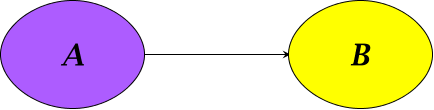
\includegraphics[width=0.5\linewidth]{images/nodes}}
\end{figure}

If your image is made up of \LaTeX\ code (for example, commands
provided by the \textsf{pgf} package) you can include it using
\cs{includeteximage} (defined by the \textsf{jmlr} class). This
can be scaled and rotated in the same way as \cs{includegraphics}.
For example, see \figureref{fig:teximage}.

\begin{figure}[htbp]
\floatconts
  {fig:teximage}
  {\caption{Image Created Using \LaTeX\ Code}}
  {\includeteximage[angle=45]{images/teximage}}
\end{figure}

If the figure is too wide to fit on the page, you can use the
\texttt{sidewaysfigure} environment defined in the
\textsf{rotating} package.

Don't use \verb|\graphicspath|.\footnote{This is specific to the
\textsf{jmlr} class, not a general recommendation. The main file
that generates the proceedings or the CiML book is typically in a
different directory to the imported articles, so it modifies the
graphics path when it imports an article.} If the images 
are contained in a subdirectory, specify this when you include the image, for
example \verb|\includegraphics{figures/mypic}|.

\subsubsection{Sub-Figures}
\label{sec:subfigures}

Sub-figures can be created using \verb|\subfigure|, which is
defined by the \textsf{jmlr} class. The optional argument allows
you to provide a subcaption. The label should be placed in the
mandatory argument of \verb|\subfigure|. You can reference the
entire figure, for example \figureref{fig:subfigex}, or you can
reference part of the figure using \verb|\figureref|, for example
\figureref{fig:circle}. Alternatively you can reference the
subfigure using \verb|\subfigref|, for example
\subfigref{fig:circle,fig:square} in \figureref{fig:subfigex}.

\begin{figure}[htbp]
\floatconts
  {fig:subfigex}
  {\caption{An Example With Sub-Figures.}}
  {%
    \subfigure[A Circle]{\label{fig:circle}%
      
\includegraphics[width=0.2\linewidth]{images/circle}}%
    \qquad
    \subfigure[A Square]{\label{fig:square}%
      
\includegraphics[width=0.2\linewidth]{images/square}}
  }
\end{figure}

By default, the sub-figures are aligned on the baseline.
This can be changed using the second optional argument
of \verb|\subfigure|. This may be \texttt{t} (top), \texttt{c}
(centered) or \texttt{b} (bottom). For example, the subfigures
\subfigref{fig:circle2,fig:square2} in \figureref{fig:subfigex2}
both have \verb|[c]| as the second optional argument.

\begin{figure}[htbp]
\floatconts
  {fig:subfigex2}
  {\caption{Another Example With Sub-Figures.}}
  {%
    \subfigure[A Small Circle][c]{\label{fig:circle2}%
      
\includegraphics[width=0.1\linewidth]{images/circle}}%
    \qquad
    \subfigure[A Square][c]{\label{fig:square2}%
      
\includegraphics[width=0.2\linewidth]{images/square}}
  }
\end{figure}

\subsection{Sub-Tables}
\label{sec:subtables}
There is an analogous command \verb|\subtable| for sub-tables.
It has the same syntax as \verb|\subfigure| described above.
You can reference the table using \verb|\tableref|, for example
\tableref{tab:subtabex} or you can reference part of the table,
for example \tableref{tab:ab}. Alternatively you can reference the
subtable using \verb|\subtabref|, for example
\subtabref{tab:ab,tab:cd} in \tableref{tab:subtabex}.

\begin{table}[htbp]
\floatconts
 {tab:subtabex}
 {\caption{An Example With Sub-Tables}}
 {%
   \subtable{%
     \label{tab:ab}%
     \begin{tabular}{cc}
     \bfseries A & \bfseries B\\
     1 & 2
     \end{tabular}
   }\qquad
   \subtable{%
     \label{tab:cd}%
     \begin{tabular}{cc}
     \bfseries C & \bfseries D\\
     3 & 4\\
     5 & 6
     \end{tabular}
   }
 }
\end{table}

By default, the sub-tables are aligned on the top.
This can be changed using the second optional argument
of \verb|\subtable|. This may be \texttt{t} (top), \texttt{c}
(centered) or \texttt{b} (bottom). For example, the sub-tables
\subtabref{tab:ab2,tab:cd2} in \tableref{tab:subtabex2}
both have \verb|[c]| as the second optional argument.

\begin{table}[htbp]
\floatconts
 {tab:subtabex2}
 {\caption{Another Example With Sub-Tables}}
 {%
   \subtable[][c]{%
     \label{tab:ab2}%
     \begin{tabular}{cc}
     \bfseries A & \bfseries B\\
     1 & 2
     \end{tabular}
   }\qquad
   \subtable[][c]{%
     \label{tab:cd2}%
     \begin{tabular}{cc}
     \bfseries C & \bfseries D\\
     3 & 4\\
     5 & 6
     \end{tabular}
   }
 }
\end{table}

\subsection{Algorithms}
\label{sec:algorithms}

Enumerated textual algorithms can be displayed using the
\texttt{algorithm} environment. Within this environment, use
\verb|\caption| to set the caption and you can use an
\texttt{enumerate} or nested \texttt{enumerate} environments.
For example, see \algorithmref{alg:gauss}. Note that algorithms
float like figures and tables.

\begin{algorithm}[htbp]
\floatconts
  {alg:gauss}%
  {\caption{The Gauss-Seidel Algorithm}}%
{%
\begin{enumerate}
  \item For $k=1$ to maximum number of iterations
    \begin{enumerate}
      \item For $i=1$ to $n$
        \begin{enumerate}
        \item $x_i^{(k)} = 
          \frac{b_i - \sum_{j=1}^{i-1}a_{ij}x_j^{(k)}
          - \sum_{j=i+1}^{n}a_{ij}x_j^{(k-1)}}{a_{ii}}$
        \item If $\|\vec{x}^{(k)}-\vec{x}^{(k-1)} < \epsilon\|$,
          where $\epsilon$ is a specified stopping criteria, stop.
      \end{enumerate}
    \end{enumerate}
\end{enumerate}
}%
\end{algorithm}

If you'd rather have the same numbering throughout the algorithm
but still want the convenient indentation of nested 
\texttt{enumerate} environments, you can use the
\texttt{enumerate*} environment provided by the \textsf{jmlr}
class. For example, see \algorithmref{alg:moore}.

\begin{algorithm}
\floatconts
  {alg:moore}%
  {\caption{Moore's Shortest Path}}%
{%
Given a connected graph $G$, where the length of each edge is 1:
\begin{enumerate*}
  \item Set the label of vertex $s$ to 0
  \item Set $i=0$
  \begin{enumerate*}
    \item \label{step:locate}Locate all unlabelled vertices 
          adjacent to a vertex labelled $i$ and label them $i+1$
    \item If vertex $t$ has been labelled,
    \begin{enumerate*}
      \item[] the shortest path can be found by backtracking, and 
      the length is given by the label of $t$.
    \end{enumerate*}
    otherwise
    \begin{enumerate*}
      \item[] increment $i$ and return to step~\ref{step:locate}
    \end{enumerate*}
  \end{enumerate*}
\end{enumerate*}
}%
\end{algorithm}

Pseudo code can be displayed using the \texttt{algorithm2e}
environment. This is defined by the \textsf{algorithm2e} package
(which is automatically loaded) so check the \textsf{algorithm2e}
documentation for further details.\footnote{Either \texttt{texdoc
algorithm2e} or \url{http://www.ctan.org/pkg/algorithm2e}}
For an example, see \algorithmref{alg:net}.

\begin{algorithm2e}
\caption{Computing Net Activation}
\label{alg:net}
 % older versions of algorithm2e have \dontprintsemicolon instead
 % of the following:
 %\DontPrintSemicolon
 % older versions of algorithm2e have \linesnumbered instead of the
 % following:
 %\LinesNumbered
\KwIn{$x_1, \ldots, x_n, w_1, \ldots, w_n$}
\KwOut{$y$, the net activation}
$y\leftarrow 0$\;
\For{$i\leftarrow 1$ \KwTo $n$}{
  $y \leftarrow y + w_i*x_i$\;
}
\end{algorithm2e}

\section{Description Lists}

The \textsf{jmlr} class also provides a description-like 
environment called \texttt{altdescription}. This has an
argument that should be the widest label in the list. Compare:
\begin{description}
\item[add] A method that adds two variables.
\item[differentiate] A method that differentiates a function.
\end{description}
with
\begin{altdescription}{differentiate}
\item[add] A method that adds two variables.
\item[differentiate] A method that differentiates a function.
\end{altdescription}

\section{Theorems, Lemmas etc}
\label{sec:theorems}

The following theorem-like environments are predefined by
the \textsf{jmlr} class: \texttt{theorem}, \texttt{example},
\texttt{lemma}, \texttt{proposition}, \texttt{remark}, 
\texttt{corollary}, \texttt{definition}, \texttt{conjecture}
and \texttt{axiom}. You can use the \texttt{proof} environment
to display the proof if need be, as in \theoremref{thm:eigenpow}.

\begin{theorem}[Eigenvalue Powers]\label{thm:eigenpow}
If $\lambda$ is an eigenvalue of $\vec{B}$ with eigenvector
$\vec{\xi}$, then $\lambda^n$ is an eigenvalue of $\vec{B}^n$
with eigenvector $\vec{\xi}$.
\begin{proof}
Let $\lambda$ be an eigenvalue of $\vec{B}$ with eigenvector
$\xi$, then
\begin{align*}
\vec{B}\vec{\xi} &= \lambda\vec{\xi}
\intertext{premultiply by $\vec{B}$:}
\vec{B}\vec{B}\vec{\xi} &= \vec{B}\lambda\vec{\xi}\\
\Rightarrow \vec{B}^2\vec{\xi} &= \lambda\vec{B}\vec{\xi}\\
&= \lambda\lambda\vec{\xi}\qquad
\text{since }\vec{B}\vec{\xi}=\lambda\vec{\xi}\\
&= \lambda^2\vec{\xi}
\end{align*}
Therefore true for $n=2$. Now assume true for $n=k$:
\begin{align*}
\vec{B}^k\vec{\xi} &= \lambda^k\vec{\xi}
\intertext{premultiply by $\vec{B}$:}
\vec{B}\vec{B}^k\vec{\xi} &= \vec{B}\lambda^k\vec{\xi}\\
\Rightarrow \vec{B}^{k+1}\vec{\xi} &= \lambda^k\vec{B}\vec{\xi}\\
&= \lambda^k\lambda\vec{\xi}\qquad
\text{since }\vec{B}\vec{\xi}=\lambda\vec{\xi}\\
&= \lambda^{k+1}\vec{\xi}
\end{align*}
Therefore true for $n=k+1$. Therefore, by induction, true for all
$n$.
\end{proof}
\end{theorem}

\begin{lemma}[A Sample Lemma]\label{lem:sample}
This is a lemma.
\end{lemma}

\begin{remark}[A Sample Remark]\label{rem:sample}
This is a remark.
\end{remark}

\begin{corollary}[A Sample Corollary]\label{cor:sample}
This is a corollary.
\end{corollary}

\begin{definition}[A Sample Definition]\label{def:sample}
This is a definition.
\end{definition}

\begin{conjecture}[A Sample Conjecture]\label{con:sample}
This is a conjecture.
\end{conjecture}

\begin{axiom}[A Sample Axiom]\label{ax:sample}
This is an axiom.
\end{axiom}

\begin{example}[An Example]\label{ex:sample}
This is an example.
\end{example}

\section{Color vs Grayscale}
\label{sec:color}

It's helpful if authors supply grayscale versions of their
images in the event that the article is to be incorporated into
a black and white printed book. With external PDF, PNG or JPG
graphic files, you just need to supply a grayscale version of the
file. For example, if the file is called \texttt{myimage.png},
then the gray version should be \texttt{myimage-gray.png} or
\texttt{myimage-gray.pdf} or \texttt{myimage-gray.jpg}. You don't
need to modify your code. The \textsf{jmlr} class checks for
the existence of the grayscale version if it is print mode 
(provided you have used \verb|\includegraphics| and haven't
specified the file extension).

You can use \verb|\ifprint| to determine which mode you are in.
For example, in \figureref{fig:nodes}, the 
\ifprint{dark gray}{purple} ellipse represents an input and the
\ifprint{light gray}{yellow} ellipse represents an output.
Another example: {\ifprint{\bfseries}{\color{red}}important text!}

You can use the class option \texttt{gray} to see how the
document will appear in gray scale mode. \textcolor{blue}{Colored
text} will automatically be converted to gray scale in print mode.

The \textsf{jmlr} class loads the \textsf{xcolor}
package, so you can also define your own colors. For example:
\ifprint
  {\definecolor{myred}{gray}{0.5}}%
  {\definecolor{myred}{rgb}{0.5,0,0}}%
\textcolor{myred}{XYZ}.

The \textsf{xcolor} class is loaded with the \texttt{x11names}
option, so you can use any of the x11 predefined colors (listed
in the \textsf{xcolor} documentation\footnote{either 
\texttt{texdoc xcolor} or \url{http://www.ctan.org/pkg/xcolor}}).

\section{Citations and Bibliography}
\label{sec:cite}

The \textsf{jmlr} class automatically loads \textsf{natbib}
and automatically sets the bibliography style, so you don't need to
use \verb|\bibliographystyle|.
This sample file has the citations defined in the accompanying
BibTeX file \texttt{jmlr-sample.bib}. For a parenthetical
citation use \verb|\citep|. For example
\citep{guyon-elisseeff-03}. For a textual citation use
\verb|\citet|. For example \citet{guyon2007causalreport}. 
Both commands may take a comma-separated list, for example
\citet{guyon-elisseeff-03,guyon2007causalreport}.

These commands have optional arguments and have a starred
version. See the \textsf{natbib} documentation for further
details.\footnote{Either \texttt{texdoc natbib} or
\url{http://www.ctan.org/pkg/natbib}}

The bibliography is displayed using \verb|\bibliography|.

\section{Introduction}
\label{sec:intro}

Conformal prediction \citep{shafer2008tutorial,vovk2005algorithmic} is a 
framework that produces predictions with accuracy guarantees.
For a given value of significance level $\epsilon \in (0;1)$, a conformal predictor is guaranteed to make exactly $\epsilon$ errors in the long run.
This is achieved at a price of a reduction in prediction precision. 
Instead of predicting a single class label, in the case of classification, or a single
number, in the case of regression, a conformal predictor outputs a range prediction, 
that is a set of class labels or an
interval that contains the true value with probability $\epsilon$.

Construction of a conformal predictor with $\epsilon = 1$ is a trivial task.
It is enough to output all class labels or an unbounded interval in case of classification and
regression respectively.
However, such a predictor is of low value, that is, it is not \textit{efficient}.
The question thus is how to guarantee the 
given level of error rate ($\epsilon$) by producing the smallest prediction regions.
This property is achieved via the definition of a proper nonconformity function that 
succeeds to measure the \textit{strangeness} or \textit{nonconformity} of every data
instance \citep{shafer2008tutorial}.

In the case of classification, the \textit{efficiency} of a conformal predictor is often measured in terms of 2 metrics: $avgC$, which stands for the average 
number of predicted class labels per instance, and $oneC$, which stands for 
the fraction of produced singleton predictions. 
Naturally, one would want to minimize $avgC$ and maximize $oneC$ at the
same time.
A recent study by \cite{johansson2017model} showed that \emph{the usage of the nonconformity
function known as \textit{margin} results in higher $oneC$ and the usage of \textit{inverse probability} (also known as $hinge$) as a nonconformal function results in lower
values of $avgC$}.
In the rest of the text, we will refer to this relationship as a baseline or original pattern
(relationship).
The authors use 21 datasets to demonstrate the statistical significance of this relationship. However, this was done for the case where the baseline classifiers were either  a single neural network (ANNs) or an ensemble of bagged ANNs. In this paper, we aim to extend this study with the following contributions:
\begin{enumerate}
    \item We study if the same pattern is present when other
    classification algorithms are used. Our experimental results with 8 
    different classifiers and 9 publicly available datasets show that although
    the previously observed pattern does hold in the majority of the cases, 
    the choice of the best nonconformity function can depend on the analyzed 
    dataset and the chosen underlying classification model. For example, 
    $k$-nearest neighbours classifier performs best with \textit{margin}.
    \textit{Margin} is also the best choice in case of \verb|balance| dataset
    regardless of the chosen classification model.

    \item We propose a method to combine both nonconformity functions. 
    Our experimental evaluation shows that this combination always results 
    in better or the same performance as \textit{inverse probability}, thus 
    allowing to increase the value of $oneC$ and decrease the value of
    $avgC$.
    In some cases, the proposed combination outperforms both 
    \textit{inverse probability} and \textit{margin} in terms of both efficiency characteristics.
    
    \item We discuss several aspects of how the accuracy of the baseline 
    classifier can impact the performance of the resulting conformal
    predictor. In particular, if the baseline prediction accuracy is very
    good, then nonconformity
    functions have no impact on the efficiency.
    Also, the accuracy of the baseline classifier strongly correlates
    with the fraction of singleton predictions that contain the true label.
    In this way, the accuracy can be an indicator of the usefulness of the $oneC$
    metric.

\end{enumerate}
 
The rest of the paper is organized as follows. In \cref{sec:literature} we discuss related works. \cref{sec:our-approach} is dedicated to the description of the proposed strategy to combine advantages of \textit{margin} and \textit{inverse probability} nonconformity functions. \cref{sec:setup} and \cref{sec:experiments} present the experimental setup and results. Finally, we summarize our work in \cref{sec:conclusions}.






\section{Related works}
\label{sec:literature}

Conformal prediction is a relatively new paradigm developed at the beginning of
2000, see \cite{linusson2021nonconformity} for an overview. It was originally developed for 
transductive setting \citep{vovk2013transductive}. The latter is efficient in terms of 
data usage but is also computationally expensive. Recent studies, including
the current one, focus on \textit{Inductive Conformal Prediction} 
(\textit{ICP})~\citep{papadopoulos2008inductive}. \textit{ICP} trains the 
learning model only once, however a part of the training dataset should be put
aside for model calibration using a predefined nonconformity function.

There are two groups of nonconformity functions: \textit{model-agnostic} and 
\textit{model-dependent}. Model-dependent nonconformity functions are defined
based on the underlying prediction model. Such functions can depend on the
distance to the separating hyperplane in SVM~\citep{balasubramanian2009support}, 
or the distance between instances in KNN classifier~\citep{proedrou2002transductive}.
These nonconformity functions are model-specific, thereby, one can not draw 
generalized conclusions about their behaviour. In a recent study by 
\cite{johansson2017model} it was shown that model-agnostic nonconformity 
functions do have some general characteristics. \textit{Inverse probability} 
nonconformity function, also knows as \textit{hinge}, is defined by the
equation $\Delta \left[ h (\vec{x_i}), y_i \right] = 1 - \hat{P}_h(y_i | \vec{x_i})$, where 
$\vec{x_i}$ is the analyzed data instance, $y_i$ is a tentative class label, and
$\hat{P}_h(y_i | \vec{x_i})$ is the probability assigned to this label given the 
instance $\vec{x_i}$ by the underlying classifier $h$. It was shown that 
conformal classifiers based on this metric tend to generate prediction regions
of lower average length ($avgC$). At the same time, the \textit{margin} 
nonconformity function results in a larger fraction of singleton predictions
($oneC$). The latter is defined by the following formula 
$\Delta ( h \left[\vec{x_i}), y_i\right] = \max_{y \neq y_i}\hat{P}_h(y | \vec{x_i}) - \hat{P}_h(y_i | \vec{x_i})$,
and it measures how different is the probability of the label $y_i$ from 
another most probable class label. The experimental evaluations in \citep{johansson2017model}, 
however, were performed for a limited number of underlying classification models:
ANN and ensemble of bagged ANNs. To the best of our knowledge, there are no
research works dedicated to the validity analysis of the discovered pattern in the case
of other classification algorithms. To our opinion, this piece of research is
missing to draw global calculations about the characteristics of these 
nonconformity functions.

Combining characteristics of both \textit{margin} and \textit{inverse
probability} nonconformity functions is a tempting idea. 
In recent years many authors dedicated
their efforts to understand how one can generate more efficient conformal
predictions through a combination of several conformal predictors.
\cite{yang2021finite} and \cite{toccaceli2019combination} studied how to aggregate
conformal 
predictions based on different training algorithms. Various strategies were 
proposed for such combination: via $p$-values~\citep{toccaceli2017combination},
a combination of monotonic conformity scores~\citep{gauraha2018synergy},
majority voting~\citep{cherubin2019majority},  
out-of-bag calibration~\citep{linusson2020efficient}, or via 
established result in Classical Statistical Hypothesis
Testing~\citep{toccaceli2019conformal}.
The challenge of every combination of conformal predictors is to retain \textit{validity}, that is 
to achieve the empirical error rate not exceeding the predefined value $\epsilon$.
This property is usually demonstrated experimentally and some authors provide 
guidelines on which values of significance levels should be used for individual
conformal algorithms to achieve the desired validity of the resulting combination.
As opposed to these general approaches, in \cref{sec:our-approach} we
propose a procedure that is based on the 
properties of \textit{margin} and \textit{inverse probability}. We show that this approach
allows combining their characteristics, higher $oneC$ and
lower $avgC$, and retains the validity at the same time.




\section{Combination of \textit{inverse probability} and \textit{margin} nonconformity functions}
\label{sec:our-approach}

As was shown by \cite{johansson2017model}, the usage of \textit{inverse probability}
nonconformity function results in less number of predicted class labels on average 
(lower $avgC$), and \textit{margin} results in a  larger fraction of singleton 
predictions (higher $oneC$). In this section, we propose an approach to combine
these properties of the two nonconformity functions. The validity of this method
is studied empirically in \cref{sec:experiments:validity} and its efficiency is 
demonstrated in \cref{sec:experiments:efficiency}.

It is desirable to have more singleton predictions. However, if a singleton prediction
does not contain the true label, then the metric $oneC$ not only loses its
value but also becomes misleading. In \cref{sec:experiments:eff-oneC} we
demonstrate that for some datasets only a half of singleton predictions contain 
the true label. Hence, in our proposed method we decide to take the 
results produced by \textit{inverse probability} nonconformity function as 
a baseline, and then extend them with some singleton predictions resulting 
from the usage of \textit{margin}. 

The proposed procedure is the following.
\textbf{First}, we construct conformal predictors using both nonconformity 
functions separately\footnote{
See \cite{vovk2005algorithmic,shafer2008tutorial,johansson2017model} for
explanation of how conformal predictors are constructed.
}. For the conformal predictor based on \textit{inverse 
probability}, we use the value of $\epsilon$ specified by the user as the
significance level. 
For the conformal predictor based on \textit{margin}
we set the significance level equal to $\epsilon / 2$. This is done to compensate for possible erroneous singleton
predictions produced by \textit{margin} nonconformity function and to achieve the
required level or empirical error rate. \textbf{Second}, for every instance in
the testing or production dataset, we analyze the predictions generated by both 
conformal classifiers. If the conformal classifier based on \textit{margin} outputs 
a singleton and the other conformal classifier not, then the prediction is
taken from the first model. Otherwise, the output of the conformal classifier 
based on \textit{inverse probability} is used.
Such a combination will perform in the worst case the same as the conformal
predictor based on \textit{inverse probability}. Otherwise, the values of
$oneC$ and/or $avgC$ will be improved, as some non-singleton predictions will
be replaced with singletons. Thereby, in case the validity is preserved, this
combination can be considered as an improved version of the 
\textit{inverse probability} nonconformity function.

In the rest of the paper, we will use \textit{M} and \textit{IP} to refer to the 
conformal classifiers based on \textit{margin} and \textit{inverse probability}
respectively. \textit{IP\_M} will be used to refer to the combination explained
above.
%referred to as a nonconformity function, although technically it is not.
For simplicity, sometimes \textit{IP\_M} will be
referred to as a nonconformity function, although technically it is not.



\section{Experimental setup}
\label{sec:setup}

%\textcolor{red}{Give names (formulas) to all rows in \cref{tab:datasets-and-results} to reference them in the text.}

To perform experimental analysis, we used the implementation of conformal
predictors available from
\textit{nonconformist}\footnote{\url{https://github.com/donlnz/nonconformist}} Python library. 
We followed the general experimental setup from the original paper by \citet{johansson2017model}.
That is we used 10x10-fold cross-validation with 90\% of the data used for 
training and validation of the model, and 10\% used for testing.
The training dataset was further split into a proper training set and a 
calibration set in proportion 4:1, i.e., 80\% of the training set was used for
actual training of the classification model, and the rest 20\% were used 
for calibration.
All the results reported below are averaged over the 10x10 folds.

In the original study, the authors used
21 publicly available multi-class datasets from UCI repository~\cite{Dua:2019}.
In this paper, we present not aggregated, but detailed results for every analyzed
dataset. That is why we chose 9 representative datasets with different
characteristics from the original list of 21 ones. 
The general information about these datasets, such as the number of instances, attributes, and defined classes is given in the first section of \cref{tab:datasets-and-results}.

\begin{sidewaystable}[htbp]
%\scriptsize
\floatconts
  {tab:datasets-and-results}
  {\caption{Characteristics of the datasets and summarization of results}}
  {
\begin{tabular}{l|l|l|l|l|l|l|l|l|l|l|l}
                             \multicolumn{3}{r|}{\textbf{Datasets} }                                & \textbf{iris} & \textit{user} & \textbf{glass} & \textit{cars} & \textbf{wave} & \textbf{balance} & \textit{wineR} & \textit{wineW} & \textit{yeast}            \\
\hline
\hline
\hline
\multirow{4}{*}{1} & \multirow{4}{*}{\rotatebox[origin=c]{90}{info}} & \# instances                    & 150           & 403           & 214            & 1728          & 5000          & 625              & 1599           & 4898           & 1484                      \\
                            & & \# attributes                   & 4             & 5             & 9              & 6             & 21            & 4                & 11             & 11             & 8                         \\
                            & & \# classes                      & 3             & 4             & 6              & 4             & 3             & 3                & 6              & 7              & 10                        \\
                            & & balanced                        & Y             & mostly        & N              & N             & Y             & N                & N              & N              & N                         \\
\hline
\hline
\hline
\multirow{2}{*}{2} & \multicolumn{2}{l|}{$b\_err$ range, \%}                           & 2-6           & 5-32          & 24-92          & 7-96          & 13-25         & 3-21             & 38-50          & 45-58          & 40-87                     \\
& \multicolumn{2}{l|}{$b\_err$ median, \%}                          & 4             & 7             & 48             & 13            & 17            & 10               & 45             & 53             & 44                        \\
\hline
\hline
\hline
\multirow{3}{*}{3} & \multirow{3}{*}{\rotatebox[origin=c]{90}{ $E\_oneC$}} & mean                      & 0.98          & 0.93          & 0.63           & 0.88          & 0.90          & 0.96             & 0.52           & 0.50           & 0.56                      \\
                            & & mean-std                        & 0.00          & 0.00          & 0.02           & 0.00          & 0.00          & 0.00             & 0.03           & 0.02           & 0.02                      \\
                            & & corr. $b\_acc$               & 0.92          & 0.98          & 0.69           & 0.93          & 0.92          & 0.80             & 0.27           & 0.78           & 0.97                      \\
\hline
\hline
\hline
\multirow{4}{*}{4}& \multirow{2}{*}{\rotatebox[origin=c]{90}{thres.}}      & $oneC$,\%                       & 5             & 15            & 75             & 47.5          & 25            & 67.5             & 72.5           & 65             & 77.5                      \\
                            & & $avgC$,\%                       & 2.5           & 22.5          & 67.5           & 37.5          & 27.5          & 42.5             & 80             & 77.5           & 82.5                      \\\cline{2-12}
%\hline
&\multirow{2}{*}{\rotatebox[origin=c]{90}{stat.}}       & $oneC$,\%                       &               & 5             & 50             & 45            & 30            & 55               & 82.5           & 85             & 85                        \\
                            & & $avgC$,\%                       &               & 17.5          & 37.5           & 45            & 47.5          & 50               & 82.5           & 77.5           & 77.5                      \\
\hline
\hline
\hline
\multirow{6}{*}{5} &\multirow{6}{*}{\rotatebox[origin=c]{90}{patterns}}    & \multirow{3}{*}{\textit{M} is the best} &               & {\scriptsize \textbf{KNN}}           & {\scriptsize \textbf{\textbf{KNN}},}        & {\scriptsize \textbf{\textbf{KNN}}}           & {\scriptsize Ada}         & {\scriptsize \textbf{\textbf{KNN}}, DT, RF,}    & {\scriptsize \textbf{\textbf{KNN}}}            & { \scriptsize \textbf{\textbf{KNN}}}            & {\scriptsize \textbf{\textbf{KNN}}(0.05, 0.1, 0.15),}     \\
                             &&                                 &               &               & {\scriptsize DT}               &               & {\scriptsize (0.1, 
                             0.15,}      & {\scriptsize GNP, MPR,}        & \scriptsize{(0.05, 0.1),}    & {\scriptsize (0.05, 0.1)}     & {\scriptsize DT(0.05), Ada(0.15,} \\
                             &&                                 &               &               &                &               & {\scriptsize 0.20)}   & {\scriptsize Ada, QDA }         & {\scriptsize DT(0.05) }      &                & {\scriptsize  0.2), QDA(0.15, 0.2)}            \\\cline{3-12}
                             && \textit{IP} is the best                      &               & {\scriptsize Ada(0.15)}     &                &               & {\scriptsize Ada(0.01)}     &                  &                &                &                           \\\cline{3-12}
                             && \textit{IP\_M} is the best                   &               &               & {\scriptsize MPR}            & {\scriptsize RF}           & {\scriptsize RF }          &                  &                &                &                           \\\cline{3-12}
                             && \textit{IP\_M} $>$ \textit{IP}               & Y             & Y             & Y              & Y             & Y             & Y                & Y              & Y              & Y\\    
\hline
\hline
\hline
%6 & \multicolumn{2}{l|}{credibility \& $b\_err$}                       & Y              & Y          %   &                & Y             & Y             & Y                &                &            %    &                           \\
%\hline
%\hline
%\hline
%                             7 & \multicolumn{2}{c|}{$b\_acc \uparrow \Rightarrow $ eff. $\uparrow$}                & ?             & ?             & ?              & ?             & ?             & ?                & ?              & ?              & ?\\
\end{tabular}
  }
\end{sidewaystable}


The original study by \citet{johansson2017model} analyzed the performance of 
conformal classifiers based on the ANN classification model.
In this paper, we aim to further extend this analysis and use 8 different
classification algorithms as baseline models: Support Vector Machine (SVM), Decision Tree (DT), $k$-Nearest Neighbours (KNN), AdaBoost (Ada), Gaussian Naive Bayes (GNB), Multilayer Perceptron (MPR), Random Forest (RF) and Quadratic Discriminant Analysis (QDA). We used implementations of these algorithms
available from the  \textit{scikit-learn} Python library. In \cref{tab:algo-params},
we summarize the input parameters of these algorithms unless the default values 
are used.

\begin{table}[htbp]
 % The first argument is the label.
 % The caption goes in the second argument, and the table contents
 % go in the third argument.
\floatconts
  {tab:algo-params}%
  {\caption{Input parameters of classification algorithms}}%
  {
\begin{tabular}{l|l}
Algorithm & Input parameters                                               \\
\hline
SVM       & probability=True                                               \\
DT        & min\_samples\_split=max(5,  5\% of proper training dataset) \\
KNN       & n\_neighbors=5                                                 \\
MPR       & alpha=1, max\_iter=1000                                        \\
RF        & n\_estimators=10, min\_samples\_split=0                         
\end{tabular}
  }
\end{table}

Different classifiers perform differently on different datasets.
We demonstrate this in the second section of \cref{tab:datasets-and-results}.
To calculate the corresponding values, we used the same 10x10-fold cross-validation but without splitting the training set into a proper training set and a
validation set.
\textit{$b\_err$ range} from the first row of this section demonstrates the range of
errors produced by all 8 classification algorithms in the baseline mode\footnote{
In this text we use the \textit{baseline mode} to refer to the standard (non-conformal) prediction.
}. We can 
notice that some datasets are easier to classify, for example, the \verb|iris| dataset for which  the maximum error is 6\%. 
At the same time, other datasets are more difficult, for example, \verb|wineW| for which none of the classifiers can produce error less than 45\%.
The performance of classifiers is not uniformly distributed within the given ranges.
This can be seen from the median of baseline error distribution, see row \textit{$b\_err$ median}.
For example, for the  \verb|cars| dataset different classifiers result in errors ranging from 7\% to 96\%. However, the median value of 13 shows that half of them perform relatively well.

%For our analysis we used 3 nonconformity functions: 1) inverse probability, \textit{IP} (also known as \textit{hinge}) defined by the following formula $\Delta \left[h \left( \vec{x_i}, y_i \right) \right] = 1 - \hat{P}_h\left(y_i | \vec{x_i} \right)$; 2) margin (\textit{M}) defined by equation $\Delta \left[h \left( \vec{x_i}, y_i \right) \right] = \max_{y \neq y_i} \hat{P}_h\left(y | \vec{x_i} \right) - \hat{P}_h\left(y_i | \vec{x_i} \right)$; 3) and the combination of \textit{inverse probability} and \textit{margin} as defined in \cref{sec:our-approach}.

All experimental evaluations were performed for 5 different values of significance
level $\epsilon \in \left\{ 0.01, 0.05, 0.1, 0.15, 0.20 \right\}$. For every 
combination of dataset, baseline classification algorithm and $\epsilon$, we 
calculated the values of $oneC$ and $avgC$ with 2 different nonconformity 
functions (\textit{IP} and \textit{M}) and their combination \textit{IP\_M}.
After that, the results were compared to see if any of the nonconformity 
functions or their combination 
results in a more efficient conformal predictor. 
Due to the space limitations of this paper, we present 
detailed results only for 4 datasets highlighted in bold in \cref{tab:datasets-and-results}. 
However, experimental results for all datasets together with the 
code used for the experimentation
are available in the related git repository\footnote{
\url{https://github.com/marharyta-aleksandrova/copa-2021-conformal-learning}
}.

%\citet{johansson2017model}

%\citep{johansson2017model}

\section{Experimental results}
\label{sec:experiments}

\subsection{Validity}
\label{sec:experiments:validity}

We start with the analysis of \textit{validity}, that is first we check if 
the produced conformal predictors indeed achieve the required error rate. 
This property was demonstrated in previous works both for \textit{inverse probability} and \textit{margin}.
It is also theoretically guaranteed for any nonconformity function, but not
for a combination of those, like \textit{IP\_M}.
In \cref{tab:validity} we demonstrate the empirical error rates averaged among all datasets. 
As we can see, all conformal predictors are well-calibrated. 
The validity of conformal predictor based on \textit{IP\_M} can be explained 
by the fact, that we add \textit{margin}-based predictions to the 
\textit{IP}-based model only in case when we are very confident about them. 
Recall that the  significance level is set to $\epsilon / 2$ for this case, see
\cref{sec:our-approach}. 
Thereby, the probability to generate enough invalid predictions to surpass 
the allowed error rate $\epsilon$ is very low.

\begin{table}[htbp]
 % The first argument is the label.
 % The caption goes in the second argument, and the table contents
 % go in the third argument.
\floatconts
  {tab:validity}%
  {\caption{Emperical error rates}}%
  {
 %\begin{wraptable}{r}{8cm}
\begin{tabular}{l|lllll}
\multicolumn{1}{r}{\textbf{eps:}}   & \textbf{0.01} & \textbf{0.05} & \textbf{0.10} & \textbf{0.15} & \textbf{0.20} \\
\hline
\textit{IP}    & 0.01          & 0.05          & 0.09         & 0.14          & 0.19         \\
\textit{IP\_M} & 0.01          & 0.05          & 0.10         & 0.15          & 0.19         \\
\textit{M}     & 0.01          & 0.05          & 0.10         & 0.15          & 0.19        
\end{tabular}
%\end{wraptable}
  }
\end{table}


%\begin{table}[htbp]
 % The first argument is the label.
 % The caption goes in the second argument, and the table contents
 % go in the third argument.
%\floatconts
%  {tab:validity}%
%  {\caption{Emperical error rates}}%
%  {
%\begin{tabular}{l|llllll}
%\textbf{eps}   & \textbf{0.01} & \textbf{0.03} & \textbf{0.05} & \textbf{0.10} & \textbf{0.15} & \textbf{0.20} \\
%\hline
%\textit{IP}    & 0.01          & 0.03          & 0.05          & 0.09         & 0.14          & 0.19         \\
%\textit{IP\_M} & 0.01          & 0.03          & 0.05          & 0.10         & 0.15          & 0.19         \\
%\textit{M}     & 0.01          & 0.03          & 0.05          & 0.10         & 0.15          & 0.19        
%\end{tabular}
%  }
%\end{table}

\subsection{Informativeness of $oneC$}
\label{sec:experiments:eff-oneC}

In \cref{sec:our-approach}, we discussed the issue that can happen with $oneC$ 
metric. Indeed, if a large portion of predicted singletons does not contain the 
true label, then this metric can be misleading.
We calculated the ratio of the number of singleton predictions that contain 
the true label to the overall number of singleton predictors for different
setups and algorithms. We denote this value as $E\_oneC$ from \textit{effective $oneC$}. The corresponding results are presented in 
section 3 of \cref{tab:datasets-and-results}.

%First, we calculated the ratio of the number of correct singleton predictors to the total number of singleton predictors produced by a conformal classifier. 
The first row of this section shows the averaged value of $E\_oneC$ over all 5
values of $\epsilon$ and 3 nonconformity functions.
We can notice that this value is very different for different datasets ranging
from 0.98 for \verb|iris| to only 0.50 for \verb|wineW|. 
This means that for \verb|wineW| on average half of the produced singleton 
predictions do not contain the true label. In real applications, this
prediction can be more confusing than a prediction with multiple labels.

We can notice that there is a certain correlation between the mean value of 
$E\_oneC$ and the difficulty of the dataset for the baseline classifiers 
($b\_err$). 
To analyze this relationship, we calculated the value of correlation between 
the corresponding characteristics.
The results are presented in the third row \textit{corr. $b\_acc$}.
We can see that for 5 of 9 datasets (56\%) the correlation is above 0.9. 
This holds for \verb|iris|, \verb|user|, \verb|cars|, \verb|wave|, and \verb|yeast| datasets.
For 2 more datasets (\verb|balance| and \verb|wineW|), the correlation coefficient is approximately 0.8.
For the \verb|glass| dataset, it is equal to 0.69, and only for \verb|wineR| the correlation is as low as 0.27.
These results show a strong relationship between the baseline error of the underlying classification model and the correctness of singleton predictions.
%It means that for a well performing classifier, we can expect a large
%portion of singleton predictions to be correct.
%However, in case of less well performing baseline classifier, only a half of %the resulting singleton prediction might contain the true label.

Finally, to check if $E\_oneC$ depends on the chosen nonconformity function, we averaged the results separately for different non-conformity functions and then calculated the standard deviation of the resulting three values.
The corresponding results are presented in the second row \textit{mean-std}.
We notice that \textit{mean-std} is very low for all datasets.
This indicates that $eff\_oneC$ does not depend on the choice of nonconformity function.

\subsection{Efficiency of different nonconformity functions}
\label{sec:experiments:efficiency}

In this section, we study the relationship between different nonconformity functions and the effectiveness of the resulting conformal predictors. 
For every combination of a dataset, a baseline classifier, and a value of $\epsilon$,
we calculate the values of $oneC$ and $avgC$. For visual analysis, the corresponding results
are plotted in figures like \cref{fig:iris,fig:glass}. Such figures contain information about
the distribution of instances between classes (plots \textit{a}), the baseline
error rate of all classification algorithms $b\_err$ (plots \textit{b}), and the 
corresponding values of the efficiency metrics (plots from \textit{c} to \textit{j}).
The latter group of plots contains three lines corresponding to \textit{margin} (dashed line),
\textit{inverse probability} (dash and dot line) and their combination \textit{IP\_M}
(thin solid line).

Further, we evaluate how significant are the differences between different nonconformity 
functions. The corresponding results are presented in tables like \cref{tab:glass}.
Here, for every baseline classifier and value of $\epsilon$, we present a comparison matrix.
A value in the matrix shows if the row setup is better (indicated with $+$) or
worse (indicated with $-$) than the column setup. The star indicates if the 
detected difference is statistically significant\footnote{Statistical significance was 
estimated using Student's t-test with $\alpha = 0.05$.}.
To avoid too small differences, we put a sign into the matrix only if the corresponding
difference is above the threshold of 2\%\footnote{For 100\% we take the value of 1 
for $oneC$ and the total number of classes for $avgC$. These are the maximum values of
these two metrics.} or it is statistically significant.
For example, from \cref{tab:glass} we can see that \textit{margin} results in better values of $oneC$ than
\textit{IP} and \textit{IP\_M} for SVM with $\epsilon=0.05$.
These results are also statistically significant, as indicated by a *.
At the same time, for $\epsilon=0.1$ \textit{margin} improves the results of 
\textit{IP\_M} by at least 2\%.
However, this difference is not statistically significant.
Section 6 of \cref{tab:datasets-and-results} shows the fraction of setups, for which we can observe  a
difference between the performance of conformal classifiers with different nonconformity functions 
either by exceeding the threshold of 2\% (\textit{thres.}) or observing statistical significance (\textit{stat.}). 
These values are calculated as follows. For every dataset, we have 40 setups (5 values of $\epsilon$ x
8 baseline classifiers). Each such setup corresponds to one matrix for $oneC$ and one 
matrix for $avgC$ in tables like \cref{tab:glass}. 
We calculate how many of these matrices either have at least one $+$ or $-$, or have at least one
statistically significant result.
After that, the calculated number is divided over 40.
%We provide detailed analysis of the results for those datasets in \cref{tab:datasets-and-results} that are highlighted in bold. 


Using the information provided in figures like \cref{fig:glass} and tables like \cref{tab:glass},
we can analyze the efficiency of conformal classifiers for different nonconformity functions
and identify which nonconformity functions perform better.
The corresponding findings are summarized in section 4 of \cref{tab:datasets-and-results}.
This section shows the deviations from the pattern originally observed by \cite{johansson2017model}.
In our experiments we observed the following 3 deviations:
1) \textbf{\textit{M} is the best}: \textit{margin} can produce both higher values of $oneC$ and lower values of $avgC$, that is \textit{margin} is the best choice of nonconformity function;
2) \textbf{\textit{IP} is the best}: \textit{inverse probability} is the best choice of
nonconformity function;
3) \textbf{\textit{IP\_M} is the best}: the combination of \textit{M} and \textit{IP} produces 
the best results in terms of both efficiency metrics.
Additionally, our experiments show that \textit{IP\_M} never performs worse than \textit{IP} 
(\textit{IP\_M} $>$ \textit{IP}).
Note also, that we never observed the inverse pattern, that is \textit{inverse probability} resulting 
in higher values of $oneC$ and \textit{margin} resulting in lower values of $avgC$ at the same time. 
In the rest of this section, we demonstrate our main findings on the examples of 4 datasets
highlighted in bold in \cref{tab:datasets-and-results}. The general conclusions are discussed
in \cref{sec:experiments:summary}.



%\subsubsection{iris}

%Let us start the analysis for the first dataset - . 
\textbf{IRIS}. The results for \verb|iris| dataset are presented in \cref{fig:iris}. 
As we can see from the plots comparing $oneC$ and $avgC$, there is almost no difference
and all 3 nonconformity functions produce the same results.
This is also reflected in section 4 of \cref{tab:datasets-and-results}.
Only for 5\% of setups we can observe a difference in terms of $oneC$, see performance of RF in \cref{fig:iris:oneC-RF-QDA}.
The difference in $avgC$ observed even less often, only in 2.5\% of setups, see results for GNP in \cref{fig:iris:avgC-GNB-MPR}. 
Statistically significant differences are never observed.
This means that the table with the significance of results like \cref{tab:glass} for this dataset is
almost empty. That is why we do not present it in the paper.
As expected, not many patterns can be observed in this case. 
The only pattern that we observe, is \textit{IP\_M} $>$ \textit{IP}.
Note, that this dataset is perfectly balanced, see \cref{fig:iris:dist-class} and all classifiers have very good performance with maximum error not exceeding 6\%, see \cref{tab:datasets-and-results} and \cref{fig:iris:baseline-error}.
We can also notice that there is a relationship between the baseline error of the classifier and the 
efficiency of the resulting conformal predictor: better classifiers tend to produce conformal 
predictors of better quality.
The 3 worst baseline predictors DT, Ada, and RF also produce conformal predictors with lower values of $oneC$, see \cref{fig:iris:oneC-SVM-DT,fig:iris:oneC-KNN-Ada,fig:iris:oneC-RF-QDA} and larger values of $avgC$, see \cref{fig:iris:avgC-SVM-DT,fig:iris:avgC-SVM-DT,fig:iris:avgC-RF-QDA}.


\begin{figure}[htbp]
\floatconts
  {fig:iris}
  {\caption{Results for \textit{iris}: \textit{M} - dashed line,
  \textit{IP} - dash and dot line, \textit{IP\_M} - thin solid line}}
  {%
    \subfigure[Distribution between classes]{
    \label{fig:iris:dist-class}%
    \includeteximage{plots/iris-dist-class}
    }%
    \qquad
    \subfigure[Baseline error, $b\_err$]{\label{fig:iris:baseline-error}%
      \includeteximage{plots/iris-baseline-error}
      }
    \qquad
    \subfigure[$oneC$: SVM and DT]{\label{fig:iris:oneC-SVM-DT}%
      \includeteximage{plots/iris-oneC-0}
      %\includeteximage{plots/iris-dist-class}
      }
    \qquad
    \subfigure[$avgC$: SVM and DT]{\label{fig:iris:avgC-SVM-DT}%
      \includeteximage{plots/iris-avgC-0}
      }
    \qquad
    \subfigure[$oneC$: KNN and Ada]{\label{fig:iris:oneC-KNN-Ada}%
      \includeteximage{plots/iris-oneC-2}
      }
    \qquad
    \subfigure[$avgC$: KNN and Ada]{\label{fig:iris:avgC-KNN-Ada}%
      \includeteximage{plots/iris-avgC-2}
      }
    \qquad
    \subfigure[$oneC$: GNB and MPR]{\label{fig:iris:oneC-GNB-MPR}%
      \includeteximage{plots/iris-oneC-4}
      }
    \qquad
    \subfigure[$avgC$: GNB and MPR]{\label{fig:iris:avgC-GNB-MPR}%
      \includeteximage{plots/iris-avgC-4}
      }
    \qquad
    \subfigure[$oneC$: RF and QDA]{\label{fig:iris:oneC-RF-QDA}%
      \includeteximage{plots/iris-oneC-6}
      }
    \qquad
    \subfigure[$avgC$: RF and QDA]{\label{fig:iris:avgC-RF-QDA}%
      \includeteximage{plots/iris-avgC-6}
      }
  }
\end{figure}

%\subsubsection{glass}

\textbf{GLASS}.
Next, we analyze the results for \verb|glass| dataset presented in \cref{fig:glass} and 
\cref{tab:glass}. This dataset is unbalanced, see \cref{fig:glass:dist-class} and 
different classifiers have different performance with baseline error ranging from 24\% for RF to 92\%
for QDA, see \cref{fig:glass:baseline-error}. As it was observed for \verb|iris| dataset, those 
classifiers that perform better in the baseline scenario also tend to produce more efficient 
conformal predictors.
For example, see the results for RF in \cref{fig:glass:oneC-RF-QDA,fig:glass:avgC-RF-QDA}, and the 
results for KNN in \cref{fig:glass:oneC-KNN-Ada,fig:glass:avgC-KNN-Ada}.
At the same time, classifiers that perform badly in the baseline scenario produce conformal 
predictors of low quality, see results for QDA in \cref{fig:glass:oneC-RF-QDA,fig:glass:avgC-RF-QDA}.
There are also exceptions, but they are less numerous. 
For example, for this dataset the baseline performance of the DT classifier is good ($b\_err \approx 
30\%$), however, the resulting conformal classifier is less efficient than the one based on SVM with 
$b\_err > 60\%$.
For this dataset, we can also observe a clear difference in performance depending on which 
nonconformity functions is used.
This is summarized in \cref{tab:glass}. 
Analyzing the results presented in this table, we can observe the following patterns.
1) For KNN and DT-based conformal predictors \textit{margin} is the best choice of nonconformity function.
Indeed, this is reflected in \cref{fig:glass:oneC-KNN-Ada,fig:glass:oneC-SVM-DT} (\textit{margin} 
results in higher values of $oneC$) and  \cref{fig:glass:avgC-KNN-Ada,fig:glass:avgC-SVM-DT} 
(\textit{margin} also results in lower values of $avgC$).
This pattern is also shown in \cref{tab:glass} in comparison matrices corresponding to KNN and DT algorithms. 
We can see that in all comparison matrices, there is a $+$ in rows corresponding to \textit{margin}
indicating that it outperforms both \textit{IP} and \textit{IP\_M},
except $avgC$ for KNN with $\epsilon=0.2$.
2) For MPR \textit{IP\_M} is the best choice of nonconformity function. 
This is reflected in the corresponding comparison matrices of \cref{tab:glass}, from which we can see
that \textit{IP\_M} results in higher values of $oneC$ and lower values of $avgC$ at the same time.
This is also visible in \cref{fig:glass:oneC-GNB-MPR,fig:glass:avgC-GNB-MPR}.
3) Finally, we never observe \textit{IP\_M} being outperformed by \textit{IP}. In the inverse direction,
however, \textit{IP\_M} does improve the results of \textit{IP}.
For example, for SVM with $\epsilon=0.05$ or $\epsilon=0.1$ \textit{IP\_M} allows to achieve better 
values of $oneC$ and this improvement is also statistically significant.
\begin{figure}[htbp]
\floatconts
  {fig:glass}
  {\caption{Results for \textit{glass}: \textit{M} - dashed line,
  \textit{IP} - dash and dot line, \textit{IP\_M} - thin solid line}}
  {%
    \subfigure[Distribution between classes]{
    \label{fig:glass:dist-class}%
    \includeteximage{plots/glass-dist-class}
    }%
    \qquad
    \subfigure[Baseline error, $b\_err$]{\label{fig:glass:baseline-error}%
      \includeteximage{plots/glass-baseline-error}
      }
    \qquad
    \subfigure[$oneC$: SVM and DT]{\label{fig:glass:oneC-SVM-DT}%
      \includeteximage{plots/glass-oneC-0}
      %\includeteximage{plots/glass-dist-class}
      }
    \qquad
    \subfigure[$avgC$: SVM and DT]{\label{fig:glass:avgC-SVM-DT}%
      \includeteximage{plots/glass-avgC-0}
      }
    \qquad
    \subfigure[$oneC$: KNN and Ada]{\label{fig:glass:oneC-KNN-Ada}%
      \includeteximage{plots/glass-oneC-2}
      }
    \qquad
    \subfigure[$avgC$: KNN and Ada]{\label{fig:glass:avgC-KNN-Ada}%
      \includeteximage{plots/glass-avgC-2}
      }
    \qquad
    \subfigure[$oneC$: GNB and MPR]{\label{fig:glass:oneC-GNB-MPR}%
      \includeteximage{plots/glass-oneC-4}
      }
    \qquad
    \subfigure[$avgC$: GNB and MPR]{\label{fig:glass:avgC-GNB-MPR}%
      \includeteximage{plots/glass-avgC-4}
      }
    \qquad
    \subfigure[$oneC$: RF and QDA]{\label{fig:glass:oneC-RF-QDA}%
      \includeteximage{plots/glass-oneC-6}
      }
    \qquad
    \subfigure[$avgC$: RF and QDA]{\label{fig:glass:avgC-RF-QDA}%
      \includeteximage{plots/glass-avgC-6}
      }
  }
\end{figure}


\begin{table}[htbp]
\scriptsize
 % The first argument is the label.
 % The caption goes in the second argument, and the table contents
 % go in the third argument.
\floatconts
  {tab:glass}%
  {\caption{Significance of results for the \textit{glass} dataset}}%
  {
\begin{tabular}{cl|lll|lll|lll|lll|lll}
             && \multicolumn{3}{c|}{$\epsilon=0.01$} & \multicolumn{3}{c|}{$\epsilon=0.05$} & \multicolumn{3}{c|}{$\epsilon=0.1$} & \multicolumn{3}{c|}{$\epsilon=0.15$} & \multicolumn{3}{c}{$\epsilon=0.2$} \\
\hline
\hline
\hline
\multirow{3}{*}{\rotatebox[origin=c]{90}{$oneC$}}&ip           &            &            &            &            & $-$*       & $-$*       &            & $-$*       & $-$*       &            & $-$        & $-$*       &            & $-$        & $-$*        \\
&ip\_m        &            &            &            & $+$*       &            & $-$*       & $+$*       &            & $-$        & $+$        &            & $-$        & $+$        &            & $-$         \\
&m            &            &            &            & $+$*       & $+$*       &            & $+$*       & $+$        &            & $+$*       & $+$        &            & $+$*       & $+$        &             \\

\hline
\multicolumn{2}{l|}{\textbf{SVM}} & ip         & ip\_m      & m          & ip         & ip\_m      & m          & ip         & ip\_m      & m          & ip         & ip\_m      & m          & ip         & ip\_m      & m           \\
\hline
\multirow{3}{*}{\rotatebox[origin=c]{90}{$avgC$}}&ip           &            &            &            &            &            & $+$*       &            &            & $+$        &            &            &            &            &            &             \\
&ip\_m        &            &            &            &            &            & $+$*       &            &            & $+$*       &            &            & $+$        &            &            &             \\
&m            &            &            &            & $-$*       & $-$*       &            & $-$        & $-$*       &            &            & $-$        &            &            &            &             \\

\hline
\hline
\hline
\multirow{3}{*}{\rotatebox[origin=c]{90}{$oneC$}}&ip           &            &            &            &            &            &            &            &            & $-$        &            & $-$        & $-$        &            & $-$        & $-$         \\
&ip\_m        &            &            &            &            &            &            &            &            & $-$        & $+$        &            & $-$        & $+$        &            & $-$         \\
&m            &            &            &            &            &            &            & $+$        & $+$        &            & $+$        & $+$        &            & $+$        & $+$        &             \\

\hline
\multicolumn{2}{l|}{\textbf{DT}} & ip         & ip\_m      & m          & ip         & ip\_m      & m          & ip         & ip\_m      & m          & ip         & ip\_m      & m          & ip         & ip\_m      & m           \\
\hline
\multirow{3}{*}{\rotatebox[origin=c]{90}{$avgC$}}&ip           &            &            &            &            &            &            &            &            & $-$        &            &            & $-$        &            &            & $-$         \\
&ip\_m        &            &            &            &            &            &            &            &            & $-$        &            &            & $-$        &            &            & $-$         \\
&m            &            &            &            &            &            &            & $+$        & $+$        &            & $+$        & $+$        &            & $+$        & $+$        &             \\

\hline
\hline
\hline
\multirow{3}{*}{\rotatebox[origin=c]{90}{$oneC$}}&ip           &            &            &            &            & $-$        & $-$*       &            & $-$        & $-$*       &            & $-$        & $-$*       &            & $-$        & $-$*        \\
&ip\_m        &            &            &            & $+$        &            & $-$        & $+$        &            & $-$        & $+$        &            & $-$*       & $+$        &            & $-$         \\
&m            &            &            &            & $+$*       & $+$        &            & $+$*       & $+$        &            & $+$*       & $+$*       &            & $+$*       & $+$        &             \\

\hline
\multicolumn{2}{l|}{\textbf{KNN}} & ip         & ip\_m      & m          & ip         & ip\_m      & m          & ip         & ip\_m      & m          & ip         & ip\_m      & m          & ip         & ip\_m      & m           \\
\hline
\multirow{3}{*}{\rotatebox[origin=c]{90}{$avgC$}}&ip           &            &            &            &            & $-$        & $-$        &            & $-$        & $-$        &            & $-$        & $-$        &            &            & $-$         \\
&ip\_m        &            &            &            & $+$        &            & $-$        & $+$        &            & $-$        & $+$        &            & $-$        &            &            &             \\
&m            &            &            &            & $+$        & $+$        &            & $+$        & $+$        &            & $+$        & $+$        &            & $+$        &            &             \\

\hline
\hline
\hline
\multirow{3}{*}{\rotatebox[origin=c]{90}{$oneC$}}&ip           &            &            &            &            &            &            &            &            & $-$*       &            &            & $-$*       &            & $-$*       & $-$*        \\
&ip\_m        &            &            &            &            &            &            &            &            & $-$        &            &            & $-$*       & $+$*       &            & $-$*        \\
&m            &            &            &            &            &            &            & $+$*       & $+$        &            & $+$*       & $+$*       &            & $+$*       & $+$*       &             \\

\hline
\multicolumn{2}{l|}{\textbf{Ada}} & ip         & ip\_m      & m          & ip         & ip\_m      & m          & ip         & ip\_m      & m          & ip         & ip\_m      & m          & ip         & ip\_m      & m           \\
\hline
\multirow{3}{*}{\rotatebox[origin=c]{90}{$avgC$}}&ip           &            &            &            &            &            & $+$*       &            &            & $+$*       &            &            & $+$*       &            &            & $+$*        \\
&ip\_m        &            &            &            &            &            & $+$*       &            &            & $+$*       &            &            & $+$*       &            &            & $+$*        \\
&m            &            &            &            & $-$*       & $-$*       &            & $-$*       & $-$*       &            & $-$*       & $-$*       &            & $-$*       & $-$*       &             \\

\hline
\hline
\hline
\multirow{3}{*}{\rotatebox[origin=c]{90}{$oneC$}}&ip           &            &            &            &            &            & $-$        &            & $-$        & $-$*       &            &            & $-$*       &            & $-$        & $-$*        \\
&ip\_m        &            &            &            &            &            &            & $+$        &            & $-$*       &            &            & $-$*       & $+$        &            & $-$*        \\
&m            &            &            &            & $+$        &            &            & $+$*       & $+$*       &            & $+$*       & $+$*       &            & $+$*       & $+$*       &             \\

\hline
\multicolumn{2}{l|}{\textbf{GNB}} & ip         & ip\_m      & m          & ip         & ip\_m      & m          & ip         & ip\_m      & m          & ip         & ip\_m      & m          & ip         & ip\_m      & m           \\
\hline
\multirow{3}{*}{\rotatebox[origin=c]{90}{$avgC$}}&ip           &            &            &            &            &            & $+$        &            &            & $+$*       &            &            & $+$*       &            &            & $+$*        \\
&ip\_m        &            &            &            &            &            & $+$        &            &            & $+$*       &            &            & $+$*       &            &            & $+$*        \\
&m            &            &            &            & $-$        & $-$        &            & $-$*       & $-$*       &            & $-$*       & $-$*       &            & $-$*       & $-$*       &             \\

\hline
\hline
\hline
\multirow{3}{*}{\rotatebox[origin=c]{90}{$oneC$}}&ip           &            &            &            &            & $-$        &            &            & $-$        & $-$        &            & $-$        &            &            & $-$        &             \\
&ip\_m        &            &            &            & $+$        &            & $+$        & $+$        &            & $+$        & $+$        &            & $+$        & $+$        &            & $+$         \\
&m            &            &            &            &            & $-$        &            & $+$        & $-$        &            &            & $-$        &            &            & $-$        &             \\

\hline
\multicolumn{2}{l|}{\textbf{MPR}} & ip         & ip\_m      & m          & ip         & ip\_m      & m          & ip         & ip\_m      & m          & ip         & ip\_m      & m          & ip         & ip\_m      & m           \\
\hline
\multirow{3}{*}{\rotatebox[origin=c]{90}{$avgC$}}&ip           &            &            &            &            &            & $+$*       &            & $-$        & $+$*       &            & $-$        & $+$*       &            & $-$        & $+$         \\
&ip\_m        &            &            &            &            &            & $+$*       & $+$        &            & $+$*       & $+$        &            & $+$*       & $+$        &            & $+$*        \\
&m            &            &            &            & $-$*       & $-$*       &            & $-$*       & $-$*       &            & $-$*       & $-$*       &            & $-$        & $-$*       &             \\

\hline
\hline
\hline
\multirow{3}{*}{\rotatebox[origin=c]{90}{$oneC$}}&ip           &            &            &            &            & $-$        & $-$*       &            & $-$        & $-$*       &            & $-$        & $-$*       &            & $-$        & $-$*        \\
&ip\_m        &            &            &            & $+$        &            &            & $+$        &            & $-$        & $+$        &            & $-$        & $+$        &            & $-$         \\
&m            &            &            &            & $+$*       &            &            & $+$*       & $+$        &            & $+$*       & $+$        &            & $+$*       & $+$        &             \\

\hline
\multicolumn{2}{l|}{\textbf{RF}} & ip         & ip\_m      & m          & ip         & ip\_m      & m          & ip         & ip\_m      & m          & ip         & ip\_m      & m          & ip         & ip\_m      & m           \\
\hline
\multirow{3}{*}{\rotatebox[origin=c]{90}{$avgC$}}&ip           &            &            &            &            & $-$        & $+$        &            &            & $+$*       &            &            & $+$        &            &            &             \\
&ip\_m        &            &            &            & $+$        &            & $+$*       &            &            & $+$*       &            &            & $+$        &            &            &             \\
&m            &            &            &            & $-$        & $-$*       &            & $-$*       & $-$*       &            & $-$        & $-$        &            &            &            &             \\

\hline
\hline
\hline
\multirow{3}{*}{\rotatebox[origin=c]{90}{$oneC$}}&ip           &            &            &            &            &            & $-$*       &            &            & $-$*       &            &            & $-$        &            &            & $-$         \\
&ip\_m        &            &            &            &            &            & $-$*       &            &            & $-$        &            &            & $-$        &            &            &             \\
&m            &            &            &            & $+$*       & $+$*       &            & $+$*       & $+$        &            & $+$        & $+$        &            & $+$        &            &             \\

\hline
\multicolumn{2}{l|}{\textbf{QDA}} & ip         & ip\_m      & m          & ip         & ip\_m      & m          & ip         & ip\_m      & m          & ip         & ip\_m      & m          & ip         & ip\_m      & m           \\
\hline
\multirow{3}{*}{\rotatebox[origin=c]{90}{$avgC$}}&ip           &            &            &            &            &            &            &            &            & $-$        &            &            &            &            &            &             \\
&ip\_m        &            &            &            &            &            &            &            &            &            &            &            &            &            &            & $+$         \\
&m            &            &            &            &            &            &            & $+$        &            &            &            &            &            &            & $-$        &             \\

\hline
\hline
\hline
\end{tabular}

  }
\end{table}

\textbf{WAVE.}
The results for \verb|wave| dataset are presented in \cref{fig:wave} and \cref{tab:wave}.
This dataset is balanced, see \cref{fig:wave:baseline-error}, and overall performance of classifies 
is quite good, see \cref{fig:wave:baseline-error}. There is only one classifier, DT, wich results in 
$b\_err > 20\%$. 
As it was also noted for \verb|iris|, when classifiers have good baseline performance, the 
difference between different nonconformity functions diminished.
This is reflected in the reduction of values in section 4 of \cref{tab:datasets-and-results} (25\%, 
27.5\%, 30\%, and 47.5\%) as compared to the corresponding values for \verb|glass| dataset 
(75\%, 67.5\%, 50\%, and 37.5\%).
We can observe visual differences in \cref{fig:wave} only for DT, Ada, GNB, and RF.
No difference is observed for KNN, however, despite it having a comparable value of $b\_err$. 
For this dataset, we can also see that \textit{margin} results in best performance for $\epsilon \in \{ 0.1, 0.15, 0.2\}$ when Ada classifier is used.
This improvement is also statistically significant, see \cref{tab:wave}. 
In the case of $\epsilon = 0.01$ however, the best performance is achieved by \textit{IP} nonconformity 
function, and this result is also statistically significant.
Further, \textit{IP\_M} is the best choice for RF classifier with statistical significance of the improvement in most of settings.

\begin{figure}[htbp]
\floatconts
  {fig:wave}
  {\caption{Results for \textit{wave}: \textit{M} - dashed line,
  \textit{IP} - dash and dot line, \textit{IP\_M} - thin solid line}}
  {%
    \subfigure[Distribution between classes]{
    \label{fig:wave:dist-class}%
    \includeteximage{plots/wave-dist-class}
    }%
    \qquad
    \subfigure[Baseline error, $b\_err$]{\label{fig:wave:baseline-error}%
      \includeteximage{plots/wave-baseline-error}
      }
    \qquad
    \subfigure[$oneC$: SVM and DT]{\label{fig:wave:oneC-SVM-DT}%
      \includeteximage{plots/wave-oneC-0}
      %\includeteximage{plots/wave-dist-class}
      }
    \qquad
    \subfigure[$avgC$: SVM and DT]{\label{fig:wave:avgC-SVM-DT}%
      \includeteximage{plots/wave-avgC-0}
      }
    \qquad
    \subfigure[$oneC$: KNN and Ada]{\label{fig:wave:oneC-KNN-Ada}%
      \includeteximage{plots/wave-oneC-2}
      }
    \qquad
    \subfigure[$avgC$: KNN and Ada]{\label{fig:wave:avgC-KNN-Ada}%
      \includeteximage{plots/wave-avgC-2}
      }
    \qquad
    \subfigure[$oneC$: GNB and MPR]{\label{fig:wave:oneC-GNB-MPR}%
      \includeteximage{plots/wave-oneC-4}
      }
    \qquad
    \subfigure[$avgC$: GNB and MPR]{\label{fig:wave:avgC-GNB-MPR}%
      \includeteximage{plots/wave-avgC-4}
      }
    \qquad
    \subfigure[$oneC$: RF and QDA]{\label{fig:wave:oneC-RF-QDA}%
      \includeteximage{plots/wave-oneC-6}
      }
    \qquad
    \subfigure[$avgC$: RF and QDA]{\label{fig:wave:avgC-RF-QDA}%
      \includeteximage{plots/wave-avgC-6}
      }
  }
\end{figure}






\begin{table}[htbp]
\scriptsize
 % The first argument is the label.
 % The caption goes in the second argument, and the table contents
 % go in the third argument.
\floatconts
  {tab:wave}%
  {\caption{wave dataset}}%
  {
\begin{tabular}{cl|lll|lll|lll|lll|lll}
             && \multicolumn{3}{c|}{$\epsilon=0.01$} & \multicolumn{3}{c|}{$\epsilon=0.05$} & \multicolumn{3}{c|}{$\epsilon=0.1$} & \multicolumn{3}{c|}{$\epsilon=0.15$} & \multicolumn{3}{c}{$\epsilon=0.2$} \\
\hline
\hline
\hline

\hline
\multicolumn{2}{l|}{\textbf{SVM}} & ip         & ip\_m      & m          & ip         & ip\_m      & m          & ip         & ip\_m      & m          & ip         & ip\_m      & m          & ip         & ip\_m      & m           \\
\hline

\hline
\hline
\hline

\hline
\multicolumn{2}{l|}{\textbf{DT}}  & ip         & ip\_m      & m          & ip         & ip\_m      & m          & ip         & ip\_m      & m          & ip         & ip\_m      & m          & ip         & ip\_m      & m           \\
\hline

\hline
\hline
\hline

\hline
\multicolumn{2}{l|}{\textbf{KNN}} & ip         & ip\_m      & m          & ip         & ip\_m      & m          & ip         & ip\_m      & m          & ip         & ip\_m      & m          & ip         & ip\_m      & m           \\
\hline

\hline
\hline
\hline

\hline
\multicolumn{2}{l|}{\textbf{Ada}} & ip         & ip\_m      & m          & ip         & ip\_m      & m          & ip         & ip\_m      & m          & ip         & ip\_m      & m          & ip         & ip\_m      & m           \\
\hline

\hline
\hline
\hline

\hline
\multicolumn{2}{l|}{\textbf{GNB}} & ip         & ip\_m      & m          & ip         & ip\_m      & m          & ip         & ip\_m      & m          & ip         & ip\_m      & m          & ip         & ip\_m      & m           \\
\hline

\hline
\hline
\hline

\hline
\multicolumn{2}{l|}{\textbf{MPR}} & ip         & ip\_m      & m          & ip         & ip\_m      & m          & ip         & ip\_m      & m          & ip         & ip\_m      & m          & ip         & ip\_m      & m           \\
\hline

\hline
\hline
\hline

\hline
\multicolumn{2}{l|}{\textbf{RF}}  & ip         & ip\_m      & m          & ip         & ip\_m      & m          & ip         & ip\_m      & m          & ip         & ip\_m      & m          & ip         & ip\_m      & m           \\
\hline

\hline
\hline
\hline

\hline
\multicolumn{2}{l|}{\textbf{QDA}} & ip         & ip\_m      & m          & ip         & ip\_m      & m          & ip         & ip\_m      & m          & ip         & ip\_m      & m          & ip         & ip\_m      & m           \\
\hline

\hline
\hline
\hline
\end{tabular}

  }
\end{table}



\textbf{BALANCE.}
The case of \verb|balance| dataset is very interesting, because, as we will see, for most of the 
classification models \textit{margin} is always the best choice of nonconformity function.
As reflected in \cref{tab:balance} and supported by \cref{fig:balance}, these differences
is mostly statistically significant.
The only cases for which the original pattern holds are SVM with all values of $\epsilon$ 
and QDA with $\epsilon=0.05$. For this dataset, we also observe differences between different
nonconformity functions despite the relatively good performance of many classifiers. 
%This was opposite for \textit{wave} dataset. Maybe it is related to the fact that margin is best choice here.

\begin{figure}[htbp]
\floatconts
  {fig:balance}
  {\caption{Results for \textit{balance} dataset.}}
  {%
    \subfigure[Distribution between classes]{
    \label{fig:balance:dist-class}%
    \includeteximage{plots/balance-dist-class}
    }%
    \qquad
    \subfigure[Baseline error]{\label{fig:square}%
      \includeteximage{plots/balance-baseline-error}
      }
    \qquad
    \subfigure[$oneC$: SVM and DT]{\label{fig:square}%
      \includeteximage{plots/balance-oneC-0}
      %\includeteximage{plots/balance-dist-class}
      }
    \qquad
    \subfigure[$avgC$: SVM and DT]{\label{fig:square}%
      \includeteximage{plots/balance-avgC-0}
      }
    \qquad
    \subfigure[$oneC$: KNN and Ada]{\label{fig:square}%
      \includeteximage{plots/balance-oneC-2}
      }
    \qquad
    \subfigure[$avgC$: KNN and Ada]{\label{fig:square}%
      \includeteximage{plots/balance-avgC-2}
      }
    \qquad
    \subfigure[$oneC$: GNB and MPR]{\label{fig:square}%
      \includeteximage{plots/balance-oneC-4}
      }
    \qquad
    \subfigure[$avgC$: GNB and MPR]{\label{fig:square}%
      \includeteximage{plots/balance-avgC-4}
      }
    \qquad
    \subfigure[$oneC$: RF and QDA]{\label{fig:square}%
      \includeteximage{plots/balance-oneC-6}
      }
    \qquad
    \subfigure[$avgC$: RF and QDA]{\label{fig:square}%
      \includeteximage{plots/balance-avgC-6}
      }
  }
\end{figure}
\begin{table}[htbp]
\scriptsize
 % The first argument is the label.
 % The caption goes in the second argument, and the table contents
 % go in the third argument.
\floatconts
  {tab:balance}%
  {\caption{Significance of results for the \textit{balance} dataset}}%
  {
\begin{tabular}{cl|lll|lll|lll|lll|lll}
             && \multicolumn{3}{c|}{$\epsilon=0.01$} & \multicolumn{3}{c|}{$\epsilon=0.05$} & \multicolumn{3}{c|}{$\epsilon=0.1$} & \multicolumn{3}{c|}{$\epsilon=0.15$} & \multicolumn{3}{c}{$\epsilon=0.2$} \\
\hline
\hline
\hline
\multirow{3}{*}{\rotatebox[origin=c]{90}{$oneC$}}&ip           &            &            & $-$*       &            &            & $-$*       &            &            &            &            &            &            &            &            &             \\
&ip\_m        &            &            & $-$*       &            &            & $-$*       &            &            &            &            &            &            &            &            &             \\
&m            & $+$*       & $+$*       &            & $+$*       & $+$*       &            &            &            &            &            &            &            &            &            &             \\

\hline
\multicolumn{2}{l|}{\textbf{SVM}} & ip         & ip\_m      & m          & ip         & ip\_m      & m          & ip         & ip\_m      & m          & ip         & ip\_m      & m          & ip         & ip\_m      & m           \\
\hline
\multirow{3}{*}{\rotatebox[origin=c]{90}{$avgC$}}&ip           &            &            & $+$*       &            &            &            &            &            &            &            &            &            &            &            &             \\
&ip\_m        &            &            & $+$*       &            &            &            &            &            &            &            &            &            &            &            &             \\
&m            & $-$*       & $-$*       &            &            &            &            &            &            &            &            &            &            &            &            &             \\

\hline
\hline
\hline
\multirow{3}{*}{\rotatebox[origin=c]{90}{$oneC$}}&ip           &            &            & $-$        &            & $-$        & $-$*       &            &            & $-$*       &            &            & $-$*       &            &            & $-$*        \\
&ip\_m        &            &            & $-$        & $+$        &            & $-$*       &            &            & $-$*       &            &            & $-$*       &            &            & $-$         \\
&m            & $+$        & $+$        &            & $+$*       & $+$*       &            & $+$*       & $+$*       &            & $+$*       & $+$*       &            & $+$*       & $+$        &             \\

\hline
\multicolumn{2}{l|}{\textbf{DT}} & ip         & ip\_m      & m          & ip         & ip\_m      & m          & ip         & ip\_m      & m          & ip         & ip\_m      & m          & ip         & ip\_m      & m           \\
\hline
\multirow{3}{*}{\rotatebox[origin=c]{90}{$avgC$}}&ip           &            &            &            &            & $-$        & $-$*       &            &            & $-$*       &            &            &            &            &            &             \\
&ip\_m        &            &            &            & $+$        &            & $-$*       &            &            & $-$*       &            &            &            &            &            &             \\
&m            &            &            &            & $+$*       & $+$*       &            & $+$*       & $+$*       &            &            &            &            &            &            &             \\

\hline
\hline
\hline
\multirow{3}{*}{\rotatebox[origin=c]{90}{$oneC$}}&ip           &            &            & $-$*       &            & $-$*       & $-$*       &            &            & $-$*       &            &            & $-$*       &            &            & $-$*        \\
&ip\_m        &            &            & $-$*       & $+$*       &            & $-$*       &            &            & $-$*       &            &            & $-$*       &            &            & $-$*        \\
&m            & $+$*       & $+$*       &            & $+$*       & $+$*       &            & $+$*       & $+$*       &            & $+$*       & $+$*       &            & $+$*       & $+$*       &             \\

\hline
\multicolumn{2}{l|}{\textbf{KNN}} & ip         & ip\_m      & m          & ip         & ip\_m      & m          & ip         & ip\_m      & m          & ip         & ip\_m      & m          & ip         & ip\_m      & m           \\
\hline
\multirow{3}{*}{\rotatebox[origin=c]{90}{$avgC$}}&ip           &            &            & $-$*       &            & $-$*       & $-$*       &            &            & $-$*       &            &            & $-$*       &            &            & $-$*        \\
&ip\_m        &            &            & $-$*       & $+$*       &            & $-$*       &            &            & $-$*       &            &            & $-$*       &            &            & $-$*        \\
&m            & $+$*       & $+$*       &            & $+$*       & $+$*       &            & $+$*       & $+$*       &            & $+$*       & $+$*       &            & $+$*       & $+$*       &             \\

\hline
\hline
\hline
\multirow{3}{*}{\rotatebox[origin=c]{90}{$oneC$}}&ip           &            &            & $-$*       &            & $-$*       & $-$*       &            & $-$*       & $-$*       &            & $-$*       & $-$*       &            & $-$*       & $-$*        \\
&ip\_m        &            &            & $-$*       & $+$*       &            & $-$*       & $+$*       &            & $-$*       & $+$*       &            & $-$*       & $+$*       &            &             \\
&m            & $+$*       & $+$*       &            & $+$*       & $+$*       &            & $+$*       & $+$*       &            & $+$*       & $+$*       &            & $+$*       &            &             \\

\hline
\multicolumn{2}{l|}{\textbf{Ada}} & ip         & ip\_m      & m          & ip         & ip\_m      & m          & ip         & ip\_m      & m          & ip         & ip\_m      & m          & ip         & ip\_m      & m           \\
\hline
\multirow{3}{*}{\rotatebox[origin=c]{90}{$avgC$}}&ip           &            &            & $-$*       &            & $-$*       & $-$*       &            & $-$*       & $-$*       &            & $-$*       & $-$*       &            & $-$*       & $-$*        \\
&ip\_m        &            &            & $-$*       & $+$*       &            &            & $+$*       &            &            & $+$*       &            &            & $+$*       &            &             \\
&m            & $+$*       & $+$*       &            & $+$*       &            &            & $+$*       &            &            & $+$*       &            &            & $+$*       &            &             \\

\hline
\hline
\hline
\multirow{3}{*}{\rotatebox[origin=c]{90}{$oneC$}}&ip           &            &            & $-$*       &            & $-$*       & $-$*       &            &            & $-$        &            &            &            &            &            &             \\
&ip\_m        &            &            & $-$*       & $+$*       &            & $-$*       &            &            & $-$        &            &            &            &            &            &             \\
&m            & $+$*       & $+$*       &            & $+$*       & $+$*       &            & $+$        & $+$        &            &            &            &            &            &            &             \\

\hline
\multicolumn{2}{l|}{\textbf{GNB}} & ip         & ip\_m      & m          & ip         & ip\_m      & m          & ip         & ip\_m      & m          & ip         & ip\_m      & m          & ip         & ip\_m      & m           \\
\hline
\multirow{3}{*}{\rotatebox[origin=c]{90}{$avgC$}}&ip           &            &            & $-$*       &            & $-$*       & $-$*       &            &            &            &            &            &            &            &            &             \\
&ip\_m        &            &            & $-$*       & $+$*       &            & $-$*       &            &            &            &            &            &            &            &            &             \\
&m            & $+$*       & $+$*       &            & $+$*       & $+$*       &            &            &            &            &            &            &            &            &            &             \\

\hline
\hline
\hline
\multirow{3}{*}{\rotatebox[origin=c]{90}{$oneC$}}&ip           &            &            & $-$*       &            &            & $-$        &            &            &            &            &            &            &            &            &             \\
&ip\_m        &            &            & $-$*       &            &            &            &            &            &            &            &            &            &            &            &             \\
&m            & $+$*       & $+$*       &            & $+$        &            &            &            &            &            &            &            &            &            &            &             \\

\hline
\multicolumn{2}{l|}{\textbf{MPR}} & ip         & ip\_m      & m          & ip         & ip\_m      & m          & ip         & ip\_m      & m          & ip         & ip\_m      & m          & ip         & ip\_m      & m           \\
\hline
\multirow{3}{*}{\rotatebox[origin=c]{90}{$avgC$}}&ip           &            &            & $-$*       &            &            &            &            &            &            &            &            &            &            &            &             \\
&ip\_m        &            &            & $-$*       &            &            &            &            &            &            &            &            &            &            &            &             \\
&m            & $+$*       & $+$*       &            &            &            &            &            &            &            &            &            &            &            &            &             \\

\hline
\hline
\hline
\multirow{3}{*}{\rotatebox[origin=c]{90}{$oneC$}}&ip           &            &            & $-$*       &            & $-$*       & $-$*       &            & $-$        & $-$        &            &            & $-$        &            &            &             \\
&ip\_m        &            &            & $-$*       & $+$*       &            & $-$*       & $+$        &            &            &            &            &            &            &            &             \\
&m            & $+$*       & $+$*       &            & $+$*       & $+$*       &            & $+$        &            &            & $+$        &            &            &            &            &             \\

\hline
\multicolumn{2}{l|}{\textbf{RF}} & ip         & ip\_m      & m          & ip         & ip\_m      & m          & ip         & ip\_m      & m          & ip         & ip\_m      & m          & ip         & ip\_m      & m           \\
\hline
\multirow{3}{*}{\rotatebox[origin=c]{90}{$avgC$}}&ip           &            &            & $-$*       &            & $-$*       & $-$*       &            &            &            &            &            &            &            &            &             \\
&ip\_m        &            &            & $-$*       & $+$*       &            & $-$        &            &            &            &            &            &            &            &            &             \\
&m            & $+$*       & $+$*       &            & $+$*       & $+$        &            &            &            &            &            &            &            &            &            &             \\

\hline
\hline
\hline
\multirow{3}{*}{\rotatebox[origin=c]{90}{$oneC$}}&ip           &            &            & $-$*       &            &            &            &            &            &            &            &            &            &            &            &             \\
&ip\_m        &            &            & $-$*       &            &            &            &            &            &            &            &            &            &            &            &             \\
&m            & $+$*       & $+$*       &            &            &            &            &            &            &            &            &            &            &            &            &             \\

\hline
\multicolumn{2}{l|}{\textbf{QDA}} & ip         & ip\_m      & m          & ip         & ip\_m      & m          & ip         & ip\_m      & m          & ip         & ip\_m      & m          & ip         & ip\_m      & m           \\
\hline
\multirow{3}{*}{\rotatebox[origin=c]{90}{$avgC$}}&ip           &            &            & $-$*       &            &            & $+$*       &            &            &            &            &            &            &            &            &             \\
&ip\_m        &            &            & $-$*       &            &            & $+$*       &            &            &            &            &            &            &            &            &             \\
&m            & $+$*       & $+$*       &            & $-$*       & $-$*       &            &            &            &            &            &            &            &            &            &             \\

\hline
\hline
\hline
\end{tabular}

  }
\end{table}

%\textbf{YEAST.}
%The last dataset that we will consider is \textit{yeast} with results presented in \cref{fig:yeast} and \cref{tab:yeast}.
%This dataset that has the largest number of classes (10) and it is highly unbalanced, see \
%cref{fig:yeast:dist-class}. 
%This is one of the most difficult datasets in the baseline setting with $b\_err$ ranging from 40\% for SVM and MPR to 87\% for QDA, see \cref{fig:yeast:baseline-error}.
%For this dataset, we again observe cases when \textit{margin} outperforms all other nonconformity function: KNN with $\epsilon \in \{ 0.05, 0.1, 0.15 \}$, DT with $\epsilon=0.05$, Ada with $\epsilon \in \{ 0.15, 0.2 \}$ and QDA with $\epsilon \in \{ 0.15, 0.2 \}$.
%For the majority of these cases, the difference is statistically significant, see \cref{tab:yeast}.
%For this dataset, we can also observe that \textit{IP\_M} allows to significantly improve the values
%of $oneC$ as compared to \textit{inverse probability} nonconformity function.
%It also usually improves the value of $avgC$, being the best choice in terms of this unless 
%\textit{margin} provides better results. For example, see results for SVM (\cref{fig:yeast:oneC-SVM-DT,fig:yeast:avgC-SVM-DT}), GNP and MPR (\cref{fig:yeast:oneC-GNB-MPR,fig:yeast:avgC-GNB-MPR}), and RF (\cref{fig:yeast:oneC-RF-QDA,fig:yeast:avgC-RF-QDA}).  

%

\begin{figure}[htbp]
\floatconts
  {fig:yeast}
  {\caption{Results for \textit{yeast}: \textit{M} - dashed line,
  \textit{IP} - dash and dot line, \textit{IP\_M} - thin solid line.}}
  {%
    \subfigure[Distribution between classes]{
    \label{fig:yeast:dist-class}%
    \includeteximage{plots/yeast-dist-class}
    }%
    \qquad
    \subfigure[Baseline error, $b\_err$]{\label{fig:yeast:baseline-error}%
      \includeteximage{plots/yeast-baseline-error}
      }
    \qquad
    \subfigure[$oneC$: SVM and DT]{\label{fig:yeast:oneC-SVM-DT}%
      \includeteximage{plots/yeast-oneC-0}
      %\includeteximage{plots/yeast-dist-class}
      }
    \qquad
    \subfigure[$avgC$: SVM and DT]{\label{fig:yeast:avgC-SVM-DT}%
      \includeteximage{plots/yeast-avgC-0}
      }
    \qquad
    \subfigure[$oneC$: KNN and Ada]{\label{fig:yeast:oneC-KNN-Ada}%
      \includeteximage{plots/yeast-oneC-2}
      }
    \qquad
    \subfigure[$avgC$: KNN and Ada]{\label{fig:yeast:avgC-KNN-Ada}%
      \includeteximage{plots/yeast-avgC-2}
      }
    \qquad
    \subfigure[$oneC$: GNB and MPR]{\label{fig:yeast:oneC-GNB-MPR}%
      \includeteximage{plots/yeast-oneC-4}
      }
    \qquad
    \subfigure[$avgC$: GNB and MPR]{\label{fig:yeast:avgC-GNB-MPR}%
      \includeteximage{plots/yeast-avgC-4}
      }
    \qquad
    \subfigure[$oneC$: RF and QDA]{\label{fig:yeast:oneC-RF-QDA}%
      \includeteximage{plots/yeast-oneC-6}
      }
    \qquad
    \subfigure[$avgC$: RF and QDA]{\label{fig:yeast:avgC-RF-QDA}%
      \includeteximage{plots/yeast-avgC-6}
      }
  }
\end{figure}



%\begin{table}[htbp]
\scriptsize
 % The first argument is the label.
 % The caption goes in the second argument, and the table contents
 % go in the third argument.
\floatconts
  {tab:yeast}%
  {\caption{yeast dataset}}%
  {
\begin{tabular}{cl|lll|lll|lll|lll|lll}
             && \multicolumn{3}{c|}{$\epsilon=0.01$} & \multicolumn{3}{c|}{$\epsilon=0.05$} & \multicolumn{3}{c|}{$\epsilon=0.1$} & \multicolumn{3}{c|}{$\epsilon=0.15$} & \multicolumn{3}{c}{$\epsilon=0.2$} \\
\hline
\hline
\hline

\hline
\multicolumn{2}{l|}{\textbf{SVM}} & ip         & ip\_m      & m          & ip         & ip\_m      & m          & ip         & ip\_m      & m          & ip         & ip\_m      & m          & ip         & ip\_m      & m           \\
\hline

\hline
\hline
\hline

\hline
\multicolumn{2}{l|}{\textbf{DT}}  & ip         & ip\_m      & m          & ip         & ip\_m      & m          & ip         & ip\_m      & m          & ip         & ip\_m      & m          & ip         & ip\_m      & m           \\
\hline

\hline
\hline
\hline

\hline
\multicolumn{2}{l|}{\textbf{KNN}} & ip         & ip\_m      & m          & ip         & ip\_m      & m          & ip         & ip\_m      & m          & ip         & ip\_m      & m          & ip         & ip\_m      & m           \\
\hline

\hline
\hline
\hline

\hline
\multicolumn{2}{l|}{\textbf{Ada}} & ip         & ip\_m      & m          & ip         & ip\_m      & m          & ip         & ip\_m      & m          & ip         & ip\_m      & m          & ip         & ip\_m      & m           \\
\hline

\hline
\hline
\hline

\hline
\multicolumn{2}{l|}{\textbf{GNB}} & ip         & ip\_m      & m          & ip         & ip\_m      & m          & ip         & ip\_m      & m          & ip         & ip\_m      & m          & ip         & ip\_m      & m           \\
\hline

\hline
\hline
\hline

\hline
\multicolumn{2}{l|}{\textbf{MPR}} & ip         & ip\_m      & m          & ip         & ip\_m      & m          & ip         & ip\_m      & m          & ip         & ip\_m      & m          & ip         & ip\_m      & m           \\
\hline

\hline
\hline
\hline

\hline
\multicolumn{2}{l|}{\textbf{RF}}  & ip         & ip\_m      & m          & ip         & ip\_m      & m          & ip         & ip\_m      & m          & ip         & ip\_m      & m          & ip         & ip\_m      & m           \\
\hline

\hline
\hline
\hline

\hline
\multicolumn{2}{l|}{\textbf{QDA}} & ip         & ip\_m      & m          & ip         & ip\_m      & m          & ip         & ip\_m      & m          & ip         & ip\_m      & m          & ip         & ip\_m      & m           \\
\hline

\hline
\hline
\hline
\end{tabular}

  }
\end{table}

\subsection{Summary of results}
\label{sec:experiments:summary}

In this subsection we summarize the findings from our experimental results shown in \cref{tab:datasets-and-results}.

    %\textbf{\textit{Margin} can be the best non-conformity function}. 
    As we saw, \textbf{\textit{margin} can be the best choice of nonconformity function} for some datasets (\verb|balance| dataset) or some algorithms. 
    An interesting fact is that for almost all datasets KNN-based conformal predictor works best with \textit{margin} in terms of both $oneC$ and $avgC$.
    %For \textit{yeast} dataset this is also observed for 3 of 4 values of $\epsilon$ which results in different values of efficiency metrics, see \cref{tab:yeast}. 
    This pattern was not observed only for \verb|iris| and \verb|wave| datasets as all 
    nonconfomity functions result in the same values of $oneC$ and $avgC$ in case KNN is used. This observation
    suggests that some classification algorithms and datasets might \textit{prefer} particular
    nonconformity functions.
    
     \textbf{\textit{Inverse probability} is almost never the best nonconformity function}.
    We observed that \textit{margin} can results in the best conformal classifiers in terms of both efficiency metrics. 
    However, it almost never happens with \textit{inverse probability} function.
    In our experiments, this was observed only for the Ada classifier for \verb|user| dataset with $\epsilon = 0.15$ and \verb|wave| dataset with $\epsilon = 0.01$.
    
     \textbf{\textit{IP\_M} improves \textit{IP}}. In none of our experiments, we  observed \textit{IP\_M} being outperformed by \textit{IP}.
    \textit{IP\_M} improves $oneC$ and $avgC$ as compared to \textit{IP} or produces the same values of these metrics.
    This is expected, as \textit{IP\_M} is basically an \textit{IP} measure with some non-singleton predictions replaced with singletons.
    This replacement naturally increases $oneC$ and decreases $avgC$.
    The fact that \textit{IP\_M} also results in valid predictions respecting the imposed value of maximum error rate $\epsilon$, as was demonstrated in \cref{tab:validity}, proves the utility of this approach.
    Additionally, in some cases \textit{IP\_M} produces better results than both \textit{margin} and \textit{inverse probability} in terms of both efficiency metrics.
    This was observed for \verb|glass| dataset with MPR, and for \verb|cars| and \textit{wave} datasets with RF.
    
    \textbf{The baseline pattern holds for the majority of the cases}. 
    In our experimental results, we discussed only the cases which deviate from the baseline pattern.
    As we saw, such cases do exist, and a
    particular nonconformity function produces the best values of both metrics for some baseline classifiers or some datasets. 
    However, in most of the cases when the difference between nonconformity functions is observed,
    \textit{margin} results in better values of $oneC$ and \textit{inverse probability} results in 
    better values of $avgC$.
    Also, we never observed an inverse pattern, that is \textit{inverse probability} resulting in 
    higher values of $oneC$ and \textit{margin} resulting in lower values of $avgC$ at the same 
    time.
    This supports the main finding of the original paper by \citet{johansson2017model}.
    
    \textbf{$oneC$ is not always useful.}
    As was discussed in \cref{sec:experiments:eff-oneC}, the metric $oneC$ can be misleading.
    For some of the datasets, only half of the singleton predictions contain the true label.
    In such cases, the minimization of $avgC$ is preferred over the maximization of $oneC$.
    We also showed that the fraction of correct singleton predictions strongly correlates with the 
    performance of the chosen classifier in the baseline scenario.
    It means that by analyzing this performance, we can estimate how accurate the singleton 
    predictors will be and we can decide which efficiency metric should be considered more important.
    Also, it was shown that the choice of nonconformity function has little impact on 
    the fraction of correct singleton predictions $E\_oneC$.
    
    \textbf{The baseline performance of the chosen classifier impacts the efficiency of the conformal predictor}.
        In our experiments, we observed that if the performance of the baseline classifier is good, then the choice of nonconformity function tends to have no impact on the efficiency of the resulting conformal classifier. This is the case for \verb|iris| and \verb|wave| datasets.
        In the case of \verb|balance| dataset, this relationship is less prominent and \textit{margin} always outperforms \textit{IP} and \textit{IP\_M}.
        This can be related to the fact that this dataset is unbalanced as opposed to the two other datasets.
        In this case, the classifier can have problems generating predictions for the minority classes. This will not be reflected in the baseline error due to the little number of instances in these classes.
        The baseline performance of the underlying classification model also has a direct impact on the efficiency of the resulting conformal classifier. 
        Except for some cases, soon after the value of $\epsilon$ reaches the value of $b\_err$,
        metric $oneC$ reaches its maximum and starts decreasing.
        At the same time, the value of $avgC$ reaches 1 and further decreases,
        see, for example, results for \verb|iris| dataset presented in \cref{fig:iris}.
        This observation makes sense.
        When $\epsilon > b\_err$, the conformal classifier is allowed to make more mistakes than it does in the baseline scenario. 
        This can be only achieved by generating empty predictions.
        For such values of $\epsilon$, more and more predictions will be singletons or empty what results in the decrease of $oneC$ and $avgC$ being below 1.





%\subsection{iris}

Results for iris dataset are presented in \cref{fig:iris} and \cref{tab:iris}. 
First of all, we can notice that the dataset is balanced and each of 3 classes contains the
same number of instances, see \cref{fig:iris:dist-class}. All classifiers perform very good on this dataset with the baseline error ranging from 0.025\% for MRP to 0.06\% for DT, see 
\cref{fig:iris:baseline-error}. The difference between the performance of difference 
non-conformity functions is only slightly visible for $oneC$ of QDA classifier 
\cref{fig:iris:oneC-RF-QDA}, and $avgC$ of MPR classifier \cref{fig:iris:avgC-GNB-MPR}.
This is also supported by the results in \cref{tab:iris}\footnote{\textcolor{red}{If iris is presented in the paper, probably we do not need to show the table, there are no significant differences}}. 
We can notice none of the nonconformity function results in statistically significant 
values of $oneC$ and $avgC$. For many cases, the obtained results are also identical. This 
holds for all setups with $\epsilon=0.01$ and for all setups with KNN classifier. The 
values of $oneC$ metric are identical for Ada, GNB and QDA classifiers, although the values
of $avgC$ are sometimes slightly different.

We can also notice that different classifiers produce conformal predictors of different
efficiency. Generally SVM, GNB, MPR and QDA classifiers produce conformal predictors of 
high efficiency with close values of $oneC$ and $avgC$. These classifiers also have lower
values of baseline error except GNB, see \cref{fig:iris:baseline-error}. On the other hand, 3 classifiers with lower accuracy, DT, ADA and RF produce classifiers of lower efficiency with DT being the worst both in accuracy and efficiency.
KNN classifier, although of having larger accuracy than SVM, also has lower efficiency when
used in conformal framework. Also, we can see that when the value of $\epsilon$ becomes larger than the baseline error of the corresponding baseline classifier, the value of $oneC$ of the relative conformal predictor starts decreasing and the value of $avgC$ is usually less than 1. This means that the confomal predictor starts producing prediction intervals with no labels. The only exception in this case is DT classifier for which the
$b\_err \approx 0.06\%$, however the described tendency occurs only for $\epsilon \ge 0.15$. 
This marks a natural boundary for \textbf{credibility} of the conformal classifiers\footnote{
\textcolor{red}{To check this. Usually credibility together with confidence is defined for every instance. Is there general credibility for the whole dataset?}
}.
When $\epsilon \approx b\_err$, we reach max of $oneC$ and $oneC \approx 1 - b\_err$ and $avgC=1$.

\begin{figure}[htbp]
\floatconts
  {fig:wave}
  {\caption{Results for \textit{wave}: \textit{M} - dashed line,
  \textit{IP} - dash and dot line, \textit{IP\_M} - thin solid line}}
  {%
    \subfigure[Distribution between classes]{
    \label{fig:wave:dist-class}%
    \includeteximage{plots/wave-dist-class}
    }%
    \qquad
    \subfigure[Baseline error, $b\_err$]{\label{fig:wave:baseline-error}%
      \includeteximage{plots/wave-baseline-error}
      }
    \qquad
    \subfigure[$oneC$: SVM and DT]{\label{fig:wave:oneC-SVM-DT}%
      \includeteximage{plots/wave-oneC-0}
      %\includeteximage{plots/wave-dist-class}
      }
    \qquad
    \subfigure[$avgC$: SVM and DT]{\label{fig:wave:avgC-SVM-DT}%
      \includeteximage{plots/wave-avgC-0}
      }
    \qquad
    \subfigure[$oneC$: KNN and Ada]{\label{fig:wave:oneC-KNN-Ada}%
      \includeteximage{plots/wave-oneC-2}
      }
    \qquad
    \subfigure[$avgC$: KNN and Ada]{\label{fig:wave:avgC-KNN-Ada}%
      \includeteximage{plots/wave-avgC-2}
      }
    \qquad
    \subfigure[$oneC$: GNB and MPR]{\label{fig:wave:oneC-GNB-MPR}%
      \includeteximage{plots/wave-oneC-4}
      }
    \qquad
    \subfigure[$avgC$: GNB and MPR]{\label{fig:wave:avgC-GNB-MPR}%
      \includeteximage{plots/wave-avgC-4}
      }
    \qquad
    \subfigure[$oneC$: RF and QDA]{\label{fig:wave:oneC-RF-QDA}%
      \includeteximage{plots/wave-oneC-6}
      }
    \qquad
    \subfigure[$avgC$: RF and QDA]{\label{fig:wave:avgC-RF-QDA}%
      \includeteximage{plots/wave-avgC-6}
      }
  }
\end{figure}




\begin{table}[htbp]
\scriptsize
 % The first argument is the label.
 % The caption goes in the second argument, and the table contents
 % go in the third argument.
\floatconts
  {tab:balance-results}%
  {\caption{balance dataset}}%
  {
\begin{tabular}{cl|lll|lll|lll|lll|lll}
             && \multicolumn{3}{c|}{$\epsilon=0.01$} & \multicolumn{3}{c|}{$\epsilon=0.05$} & \multicolumn{3}{c|}{$\epsilon=0.1$} & \multicolumn{3}{c|}{$\epsilon=0.15$} & \multicolumn{3}{c}{$\epsilon=0.2$} \\
\hline
\hline
\hline
\multirow{3}{*}{\rotatebox[origin=c]{90}{$oneC$}}&ip           &            &            & $-$*       &            & $-$        & $-$*       &            & $-$        & $-$        &            & $-$        & $-$        &            &            & $-$         \\
&ip\_m        &            &            & $-$*       & $+$        &            & $-$*       & $+$        &            & $-$        & $+$        &            & $-$        &            &            & $-$         \\
&m            & $+$*       & $+$*       &            & $+$*       & $+$*       &            & $+$        & $+$        &            & $+$        & $+$        &            & $+$        & $+$        &             \\
\hline
\multicolumn{2}{l|}{\textbf{SVM}} & ip         & ip\_m      & m          & ip         & ip\_m      & m          & ip         & ip\_m      & m          & ip         & ip\_m      & m          & ip         & ip\_m      & m           \\
\hline
\multirow{3}{*}{\rotatebox[origin=c]{90}{$avgC$}}&ip           &            &            & $+$*       &            & $-$        & $-$        &            & $-$        & $+$        &            & $-$        & $+$        &            &            & $+$         \\
&ip\_m        &            &            & $+$*       & $+$        &            & $+$        & $+$        &            & $+$        & $+$        &            & $+$        &            &            & $+$         \\
&m            & $-$*       & $-$*       &            & $+$        & $-$        &            & $-$        & $-$        &            & $-$        & $-$        &            & $-$        & $-$        &             \\
\hline
\hline
\hline
\multirow{3}{*}{\rotatebox[origin=c]{90}{$oneC$}}&ip           &            &            & $-$        &            & $-$        & $-$*       &            & $-$        & $-$*       &            & $-$        & $-$*       &            & $-$        & $-$*        \\
&ip\_m        &            &            & $-$        & $+$        &            & $-$*       & $+$        &            & $-$*       & $+$        &            & $-$*       & $+$        &            & $-$         \\
&m            & $+$        & $+$        &            & $+$*       & $+$*       &            & $+$*       & $+$*       &            & $+$*       & $+$*       &            & $+$*       & $+$        &             \\
\hline
\multicolumn{2}{l|}{\textbf{DT}}  & ip         & ip\_m      & m          & ip         & ip\_m      & m          & ip         & ip\_m      & m          & ip         & ip\_m      & m          & ip         & ip\_m      & m           \\
\hline
\multirow{3}{*}{\rotatebox[origin=c]{90}{$avgC$}}&ip           &            &            & $-$        &            & $-$        & $-$*       &            & $-$        & $-$*       &            & $-$        & $-$        &            & $-$        & $-$         \\
&ip\_m        &            &            & $-$        & $+$        &            & $-$*       & $+$        &            & $-$*       & $+$        &            & $-$        & $+$        &            & $-$         \\
&m            & $+$        & $+$        &            & $+$*       & $+$*       &            & $+$*       & $+$*       &            & $+$        & $+$        &            & $+$        & $+$        &             \\
\hline
\hline
\hline
\multirow{3}{*}{\rotatebox[origin=c]{90}{$oneC$}}&ip           &            &            & $-$*       &            & $-$*       & $-$*       &            & $-$        & $-$*       &            &            & $-$*       &            & $-$        & $-$*        \\
&ip\_m        &            &            & $-$*       & $+$*       &            & $-$*       & $+$        &            & $-$*       &            &            & $-$*       & $+$        &            & $-$*        \\
&m            & $+$*       & $+$*       &            & $+$*       & $+$*       &            & $+$*       & $+$*       &            & $+$*       & $+$*       &            & $+$*       & $+$*       &             \\
\hline
\multicolumn{2}{l|}{\textbf{KNN}} & ip         & ip\_m      & m          & ip         & ip\_m      & m          & ip         & ip\_m      & m          & ip         & ip\_m      & m          & ip         & ip\_m      & m           \\
\hline
\multirow{3}{*}{\rotatebox[origin=c]{90}{$avgC$}}&ip           &            &            & $-$*       &            & $-$*       & $-$*       &            & $-$        & $-$*       &            &            & $-$*       &            & $-$        & $-$*        \\
&ip\_m        &            &            & $-$*       & $+$*       &            & $-$*       & $+$        &            & $-$*       &            &            & $-$*       & $+$        &            & $-$*        \\
&m            & $+$*       & $+$*       &            & $+$*       & $+$*       &            & $+$*       & $+$*       &            & $+$*       & $+$*       &            & $+$*       & $+$*       &             \\
\hline
\hline
\hline
\multirow{3}{*}{\rotatebox[origin=c]{90}{$oneC$}}&ip           &            &            & $-$*       &            & $-$*       & $-$*       &            & $-$*       & $-$*       &            & $-$*       & $-$*       &            & $-$*       & $-$*        \\
&ip\_m        &            &            & $-$*       & $+$*       &            & $-$*       & $+$*       &            & $-$*       & $+$*       &            & $-$*       & $+$*       &            & $-$         \\
&m            & $+$*       & $+$*       &            & $+$*       & $+$*       &            & $+$*       & $+$*       &            & $+$*       & $+$*       &            & $+$*       & $+$        &             \\
\hline
\multicolumn{2}{l|}{\textbf{Ada}} & ip         & ip\_m      & m          & ip         & ip\_m      & m          & ip         & ip\_m      & m          & ip         & ip\_m      & m          & ip         & ip\_m      & m           \\
\hline
\multirow{3}{*}{\rotatebox[origin=c]{90}{$avgC$}}&ip           &            &            & $-$*       &            & $-$*       & $-$*       &            & $-$*       & $-$*       &            & $-$*       & $-$*       &            & $-$*       & $-$*        \\
&ip\_m        &            &            & $-$*       & $+$*       &            & $-$        & $+$*       &            & $+$        & $+$*       &            & $+$        & $+$*       &            & $+$         \\
&m            & $+$*       & $+$*       &            & $+$*       & $+$        &            & $+$*       & $-$        &            & $+$*       & $-$        &            & $+$*       & $-$        &             \\
\hline
\hline
\hline
\multirow{3}{*}{\rotatebox[origin=c]{90}{$oneC$}}&ip           &            &            & $-$*       &            & $-$*       & $-$*       &            & $-$        & $-$        &            &            & $-$        &            &            & $-$         \\
&ip\_m        &            &            & $-$*       & $+$*       &            & $-$*       & $+$        &            & $-$        &            &            & $-$        &            &            & $-$         \\
&m            & $+$*       & $+$*       &            & $+$*       & $+$*       &            & $+$        & $+$        &            & $+$        & $+$        &            & $+$        & $+$        &             \\
\hline
\multicolumn{2}{l|}{\textbf{GNB}} & ip         & ip\_m      & m          & ip         & ip\_m      & m          & ip         & ip\_m      & m          & ip         & ip\_m      & m          & ip         & ip\_m      & m           \\
\hline
\multirow{3}{*}{\rotatebox[origin=c]{90}{$avgC$}}&ip           &            &            & $-$*       &            & $-$*       & $-$*       &            & $-$        & $-$        &            &            & $+$        &            &            & $+$         \\
&ip\_m        &            &            & $-$*       & $+$*       &            & $-$*       & $+$        &            & $-$        &            &            & $+$        &            &            & $+$         \\
&m            & $+$*       & $+$*       &            & $+$*       & $+$*       &            & $+$        & $+$        &            & $-$        & $-$        &            & $-$        & $-$        &             \\
\hline
\hline
\hline
\multirow{3}{*}{\rotatebox[origin=c]{90}{$oneC$}}&ip           &            &            & $-$*       &            & $-$        & $-$        &            & $-$        & $-$        &            &            & $-$        &            &            & $-$         \\
&ip\_m        &            &            & $-$*       & $+$        &            & $-$        & $+$        &            & $-$        &            &            & $-$        &            &            & $-$         \\
&m            & $+$*       & $+$*       &            & $+$        & $+$        &            & $+$        & $+$        &            & $+$        & $+$        &            & $+$        & $+$        &             \\
\hline
\multicolumn{2}{l|}{\textbf{MPR}} & ip         & ip\_m      & m          & ip         & ip\_m      & m          & ip         & ip\_m      & m          & ip         & ip\_m      & m          & ip         & ip\_m      & m           \\
\hline
\multirow{3}{*}{\rotatebox[origin=c]{90}{$avgC$}}&ip           &            &            & $-$*       &            & $-$        & $-$        &            & $-$        & $-$        &            &            & $+$        &            &            & $+$         \\
&ip\_m        &            &            & $-$*       & $+$        &            & $-$        & $+$        &            & $-$        &            &            & $+$        &            &            & $+$         \\
&m            & $+$*       & $+$*       &            & $+$        & $+$        &            & $+$        & $+$        &            & $-$        & $-$        &            & $-$        & $-$        &             \\
\hline
\hline
\hline
\multirow{3}{*}{\rotatebox[origin=c]{90}{$oneC$}}&ip           &            &            & $-$*       &            & $-$*       & $-$*       &            & $-$        & $-$        &            & $-$        & $-$        &            & $-$        & $-$         \\
&ip\_m        &            &            & $-$*       & $+$*       &            & $-$*       & $+$        &            & $-$        & $+$        &            & $-$        & $+$        &            & $-$         \\
&m            & $+$*       & $+$*       &            & $+$*       & $+$*       &            & $+$        & $+$        &            & $+$        & $+$        &            & $+$        & $+$        &             \\
\hline
\multicolumn{2}{l|}{\textbf{RF}}  & ip         & ip\_m      & m          & ip         & ip\_m      & m          & ip         & ip\_m      & m          & ip         & ip\_m      & m          & ip         & ip\_m      & m           \\
\hline
\multirow{3}{*}{\rotatebox[origin=c]{90}{$avgC$}}&ip           &            &            & $-$*       &            & $-$*       & $-$*       &            & $-$        & $-$        &            & $-$        & $-$        &            & $-$        & $-$         \\
&ip\_m        &            &            & $-$*       & $+$*       &            & $-$        & $+$        &            & $+$        & $+$        &            & $+$        & $+$        &            & $-$         \\
&m            & $+$*       & $+$*       &            & $+$*       & $+$        &            & $+$        & $-$        &            & $+$        & $-$        &            & $+$        & $+$        &             \\
\hline
\hline
\hline
\multirow{3}{*}{\rotatebox[origin=c]{90}{$oneC$}}&ip           &            &            & $-$*       &            & $-$        & $-$        &            & $-$        & $+$        &            &            & $+$        &            &            & $-$         \\
&ip\_m        &            &            & $-$*       & $+$        &            & $+$        & $+$        &            & $+$        &            &            & $+$        &            &            & $-$         \\
&m            & $+$*       & $+$*       &            & $+$        & $-$        &            & $-$        & $-$        &            & $-$        & $-$        &            & $+$        & $+$        &             \\
\hline
\multicolumn{2}{l|}{\textbf{QDA}} & ip         & ip\_m      & m          & ip         & ip\_m      & m          & ip         & ip\_m      & m          & ip         & ip\_m      & m          & ip         & ip\_m      & m           \\
\hline
\multirow{3}{*}{\rotatebox[origin=c]{90}{$avgC$}}&ip           &            &            & $-$*       &            & $-$        & $+$*       &            & $-$        & $+$        &            &            & $-$        &            &            & $+$         \\
&ip\_m        &            &            & $-$*       & $+$        &            & $+$*       & $+$        &            & $+$        &            &            & $-$        &            &            & $+$         \\
&m            & $+$*       & $+$*       &            & $-$*       & $-$*       &            & $-$        & $-$        &            & $+$        & $+$        &            & $-$        & $-$        &             \\
\hline
\hline
\hline
\end{tabular}

  }
\end{table}

%\begin{table}[htbp]
\scriptsize
 % The first argument is the label.
 % The caption goes in the second argument, and the table contents
 % go in the third argument.
\floatconts
  {tab:wineW}%
  {\caption{wineW dataset}}%
  {
\begin{tabular}{cl|lll|lll|lll|lll|lll}
             && \multicolumn{3}{c|}{$\epsilon=0.01$} & \multicolumn{3}{c|}{$\epsilon=0.05$} & \multicolumn{3}{c|}{$\epsilon=0.1$} & \multicolumn{3}{c|}{$\epsilon=0.15$} & \multicolumn{3}{c}{$\epsilon=0.2$} \\
\hline
\hline
\hline
\multirow{3}{*}{\rotatebox[origin=c]{90}{$oneC$}}&ip           &            & $-$*       & $-$*       &            & $-$*       & $-$*       &            & $-$*       & $-$*       &            &            & $-$*       &            &            & $-$*        \\
&ip\_m        & $+$*       &            &            & $+$*       &            & $-$*       & $+$*       &            & $-$*       &            &            & $-$*       &            &            & $-$*        \\
&m            & $+$*       &            &            & $+$*       & $+$*       &            & $+$*       & $+$*       &            & $+$*       & $+$*       &            & $+$*       & $+$*       &             \\

\hline
\multicolumn{2}{l|}{\textbf{SVM}} & ip         & ip\_m      & m          & ip         & ip\_m      & m          & ip         & ip\_m      & m          & ip         & ip\_m      & m          & ip         & ip\_m      & m           \\
\hline
\multirow{3}{*}{\rotatebox[origin=c]{90}{$avgC$}}&ip           &            &            & $+$*       &            &            & $+$*       &            &            &            &            &            & $+$*       &            &            & $+$*        \\
&ip\_m        &            &            & $+$*       &            &            & $+$*       &            &            &            &            &            & $+$*       &            &            & $+$*        \\
&m            & $-$*       & $-$*       &            & $-$*       & $-$*       &            &            &            &            & $-$*       & $-$*       &            & $-$*       & $-$*       &             \\

\hline
\hline
\hline
\multirow{3}{*}{\rotatebox[origin=c]{90}{$oneC$}}&ip           &            & $-$*       & $-$*       &            & $-$*       & $-$*       &            & $-$*       & $-$*       &            & $-$*       & $-$*       &            &            & $-$*        \\
&ip\_m        & $+$*       &            & $-$*       & $+$*       &            & $-$*       & $+$*       &            & $-$*       & $+$*       &            & $-$*       &            &            & $-$*        \\
&m            & $+$*       & $+$*       &            & $+$*       & $+$*       &            & $+$*       & $+$*       &            & $+$*       & $+$*       &            & $+$*       & $+$*       &             \\

\hline
\multicolumn{2}{l|}{\textbf{DT}} & ip         & ip\_m      & m          & ip         & ip\_m      & m          & ip         & ip\_m      & m          & ip         & ip\_m      & m          & ip         & ip\_m      & m           \\
\hline
\multirow{3}{*}{\rotatebox[origin=c]{90}{$avgC$}}&ip           &            &            &            &            &            & $+$*       &            & $-$*       & $+$*       &            & $-$*       & $+$*       &            &            & $+$*        \\
&ip\_m        &            &            &            &            &            & $+$*       & $+$*       &            & $+$*       & $+$*       &            & $+$*       &            &            & $+$*        \\
&m            &            &            &            & $-$*       & $-$*       &            & $-$*       & $-$*       &            & $-$*       & $-$*       &            & $-$*       & $-$*       &             \\

\hline
\hline
\hline
\multirow{3}{*}{\rotatebox[origin=c]{90}{$oneC$}}&ip           &            &            &            &            & $-$*       & $-$*       &            & $-$*       & $-$*       &            & $-$*       & $-$*       &            &            & $-$*        \\
&ip\_m        &            &            &            & $+$*       &            & $-$*       & $+$*       &            &            & $+$*       &            &            &            &            & $-$*        \\
&m            &            &            &            & $+$*       & $+$*       &            & $+$*       &            &            & $+$*       &            &            & $+$*       & $+$*       &             \\

\hline
\multicolumn{2}{l|}{\textbf{KNN}} & ip         & ip\_m      & m          & ip         & ip\_m      & m          & ip         & ip\_m      & m          & ip         & ip\_m      & m          & ip         & ip\_m      & m           \\
\hline
\multirow{3}{*}{\rotatebox[origin=c]{90}{$avgC$}}&ip           &            &            &            &            & $-$        & $-$*       &            & $-$*       & $-$*       &            &            &            &            &            & $+$*        \\
&ip\_m        &            &            &            & $+$        &            & $-$        & $+$*       &            & $-$*       &            &            & $+$        &            &            & $+$*        \\
&m            &            &            &            & $+$*       & $+$        &            & $+$*       & $+$*       &            &            & $-$        &            & $-$*       & $-$*       &             \\

\hline
\hline
\hline
\multirow{3}{*}{\rotatebox[origin=c]{90}{$oneC$}}&ip           &            &            &            &            &            &            &            &            &            &            &            &            &            &            &             \\
&ip\_m        &            &            &            &            &            &            &            &            &            &            &            &            &            &            &             \\
&m            &            &            &            &            &            &            &            &            &            &            &            &            &            &            &             \\

\hline
\multicolumn{2}{l|}{\textbf{Ada}} & ip         & ip\_m      & m          & ip         & ip\_m      & m          & ip         & ip\_m      & m          & ip         & ip\_m      & m          & ip         & ip\_m      & m           \\
\hline
\multirow{3}{*}{\rotatebox[origin=c]{90}{$avgC$}}&ip           &            &            & $+$        &            &            &            &            &            &            &            &            &            &            &            & $-$         \\
&ip\_m        &            &            & $+$        &            &            &            &            &            &            &            &            &            &            &            & $-$         \\
&m            & $-$        & $-$        &            &            &            &            &            &            &            &            &            &            & $+$        & $+$        &             \\

\hline
\hline
\hline
\multirow{3}{*}{\rotatebox[origin=c]{90}{$oneC$}}&ip           &            & $-$*       & $-$*       &            & $-$*       & $-$*       &            & $-$*       & $-$*       &            & $-$*       & $-$*       &            & $-$*       & $-$*        \\
&ip\_m        & $+$*       &            & $-$*       & $+$*       &            & $-$*       & $+$*       &            & $-$*       & $+$*       &            & $-$*       & $+$*       &            & $-$*        \\
&m            & $+$*       & $+$*       &            & $+$*       & $+$*       &            & $+$*       & $+$*       &            & $+$*       & $+$*       &            & $+$*       & $+$*       &             \\

\hline
\multicolumn{2}{l|}{\textbf{GNB}} & ip         & ip\_m      & m          & ip         & ip\_m      & m          & ip         & ip\_m      & m          & ip         & ip\_m      & m          & ip         & ip\_m      & m           \\
\hline
\multirow{3}{*}{\rotatebox[origin=c]{90}{$avgC$}}&ip           &            &            & $+$*       &            &            & $+$*       &            &            & $+$*       &            & $-$*       & $+$*       &            & $-$*       & $+$*        \\
&ip\_m        &            &            & $+$*       &            &            & $+$*       &            &            & $+$*       & $+$*       &            & $+$*       & $+$*       &            & $+$*        \\
&m            & $-$*       & $-$*       &            & $-$*       & $-$*       &            & $-$*       & $-$*       &            & $-$*       & $-$*       &            & $-$*       & $-$*       &             \\

\hline
\hline
\hline
\multirow{3}{*}{\rotatebox[origin=c]{90}{$oneC$}}&ip           &            & $-$*       & $-$*       &            & $-$*       & $-$*       &            & $-$*       & $-$*       &            & $-$*       & $-$*       &            & $-$*       & $-$*        \\
&ip\_m        & $+$*       &            & $-$*       & $+$*       &            & $-$*       & $+$*       &            & $-$*       & $+$*       &            & $-$*       & $+$*       &            &             \\
&m            & $+$*       & $+$*       &            & $+$*       & $+$*       &            & $+$*       & $+$*       &            & $+$*       & $+$*       &            & $+$*       &            &             \\

\hline
\multicolumn{2}{l|}{\textbf{MPR}} & ip         & ip\_m      & m          & ip         & ip\_m      & m          & ip         & ip\_m      & m          & ip         & ip\_m      & m          & ip         & ip\_m      & m           \\
\hline
\multirow{3}{*}{\rotatebox[origin=c]{90}{$avgC$}}&ip           &            &            & $+$*       &            &            & $+$*       &            &            & $+$*       &            & $-$*       & $+$*       &            & $-$*       & $+$*        \\
&ip\_m        &            &            & $+$*       &            &            & $+$*       &            &            & $+$*       & $+$*       &            & $+$*       & $+$*       &            & $+$*        \\
&m            & $-$*       & $-$*       &            & $-$*       & $-$*       &            & $-$*       & $-$*       &            & $-$*       & $-$*       &            & $-$*       & $-$*       &             \\

\hline
\hline
\hline
\multirow{3}{*}{\rotatebox[origin=c]{90}{$oneC$}}&ip           &            & $-$*       & $-$*       &            & $-$*       & $-$*       &            & $-$*       & $-$*       &            & $-$*       & $-$*       &            & $-$*       & $-$*        \\
&ip\_m        & $+$*       &            & $-$*       & $+$*       &            & $-$*       & $+$*       &            & $-$*       & $+$*       &            & $-$*       & $+$*       &            & $-$         \\
&m            & $+$*       & $+$*       &            & $+$*       & $+$*       &            & $+$*       & $+$*       &            & $+$*       & $+$*       &            & $+$*       & $+$        &             \\

\hline
\multicolumn{2}{l|}{\textbf{RF}} & ip         & ip\_m      & m          & ip         & ip\_m      & m          & ip         & ip\_m      & m          & ip         & ip\_m      & m          & ip         & ip\_m      & m           \\
\hline
\multirow{3}{*}{\rotatebox[origin=c]{90}{$avgC$}}&ip           &            &            & $+$*       &            &            & $+$*       &            &            & $+$*       &            & $-$*       & $+$*       &            & $-$*       & $+$*        \\
&ip\_m        &            &            & $+$*       &            &            & $+$*       &            &            & $+$*       & $+$*       &            & $+$*       & $+$*       &            & $+$*        \\
&m            & $-$*       & $-$*       &            & $-$*       & $-$*       &            & $-$*       & $-$*       &            & $-$*       & $-$*       &            & $-$*       & $-$*       &             \\

\hline
\hline
\hline
\multirow{3}{*}{\rotatebox[origin=c]{90}{$oneC$}}&ip           &            & $-$*       & $-$*       &            & $-$*       & $-$*       &            & $-$*       & $-$*       &            & $-$*       & $-$*       &            &            & $-$*        \\
&ip\_m        & $+$*       &            & $-$*       & $+$*       &            & $-$*       & $+$*       &            & $-$*       & $+$*       &            & $-$*       &            &            & $-$*        \\
&m            & $+$*       & $+$*       &            & $+$*       & $+$*       &            & $+$*       & $+$*       &            & $+$*       & $+$*       &            & $+$*       & $+$*       &             \\

\hline
\multicolumn{2}{l|}{\textbf{QDA}} & ip         & ip\_m      & m          & ip         & ip\_m      & m          & ip         & ip\_m      & m          & ip         & ip\_m      & m          & ip         & ip\_m      & m           \\
\hline
\multirow{3}{*}{\rotatebox[origin=c]{90}{$avgC$}}&ip           &            &            & $+$*       &            &            & $+$*       &            &            & $+$*       &            &            & $+$*       &            &            & $+$*        \\
&ip\_m        &            &            & $+$*       &            &            & $+$*       &            &            & $+$*       &            &            & $+$*       &            &            & $+$*        \\
&m            & $-$*       & $-$*       &            & $-$*       & $-$*       &            & $-$*       & $-$*       &            & $-$*       & $-$*       &            & $-$*       & $-$*       &             \\

\hline
\hline
\hline
\end{tabular}

  }
\end{table}
%\subsection{user}

\begin{figure}[htbp]
\floatconts
  {fig:user}
  {\caption{Results for \textit{user} dataset.}}
  {%
    \subfigure[Distribution between classes]{
    \label{fig:user:dist-class}%
    \includeteximage{plots/user-dist-class}
    }%
    \qquad
    \subfigure[Baseline error]{\label{fig:square}%
      \includeteximage{plots/user-baseline-error}
      }
    \qquad
    \subfigure[$oneC$: SVM and DT]{\label{fig:square}%
      \includeteximage{plots/user-oneC-0}
      %\includeteximage{plots/user-dist-class}
      }
    \qquad
    \subfigure[$avgC$: SVM and DT]{\label{fig:square}%
      \includeteximage{plots/user-avgC-0}
      }
    \qquad
    \subfigure[$oneC$: KNN and Ada]{\label{fig:square}%
      \includeteximage{plots/user-oneC-2}
      }
    \qquad
    \subfigure[$avgC$: KNN and Ada]{\label{fig:square}%
      \includeteximage{plots/user-avgC-2}
      }
    \qquad
    \subfigure[$oneC$: GNB and MPR]{\label{fig:square}%
      \includeteximage{plots/user-oneC-4}
      }
    \qquad
    \subfigure[$avgC$: GNB and MPR]{\label{fig:square}%
      \includeteximage{plots/user-avgC-4}
      }
    \qquad
    \subfigure[$oneC$: RF and QDA]{\label{fig:square}%
      \includeteximage{plots/user-oneC-6}
      }
    \qquad
    \subfigure[$avgC$: RF and QDA]{\label{fig:square}%
      \includeteximage{plots/user-avgC-6}
      }
  }
\end{figure}


\begin{table}[htbp]
\scriptsize
 % The first argument is the label.
 % The caption goes in the second argument, and the table contents
 % go in the third argument.
\floatconts
  {tab:user-results}%
  {\caption{user dataset}}%
  {
\begin{tabular}{cl|lll|lll|lll|lll|lll}
             && \multicolumn{3}{c|}{$\epsilon=0.01$} & \multicolumn{3}{c|}{$\epsilon=0.05$} & \multicolumn{3}{c|}{$\epsilon=0.1$} & \multicolumn{3}{c|}{$\epsilon=0.15$} & \multicolumn{3}{c}{$\epsilon=0.2$} \\
\hline
\hline
\multirow{3}{*}{\rotatebox[origin=c]{90}{$oneC$}}&ip           &            &            &            &            &            & $+$        &            &            & $+$        &            &            & $-$        &            &            & $+$         \\
&ip\_m        &            &            &            &            &            & $+$        &            &            & $+$        &            &            & $-$        &            &            & $+$         \\
&m            &            &            &            & $-$        & $-$        &            & $-$        & $-$        &            & $+$        & $+$        &            & $-$        & $-$        &             \\
\hline
\multicolumn{2}{l|}{\textbf{SVM}} & ip         & ip\_m      & m          & ip         & ip\_m      & m          & ip         & ip\_m      & m          & ip         & ip\_m      & m          & ip         & ip\_m      & m           \\
\hline
\multirow{3}{*}{\rotatebox[origin=c]{90}{$avgC$}}&ip           &            &            &            &            &            & $+$*       &            &            & $-$        &            &            & $+$        &            &            & $-$         \\
&ip\_m        &            &            &            &            &            & $+$*       &            &            & $-$        &            &            & $+$        &            &            & $-$         \\
&m            &            &            &            & $-$*       & $-$*       &            & $+$        & $+$        &            & $-$        & $-$        &            & $+$        & $+$        &             \\
\hline
\hline
\multirow{3}{*}{\rotatebox[origin=c]{90}{$oneC$}}&ip           &            &            &            &            &            & $-$        &            &            & $-$        &            &            & $+$        &            &            & $+$         \\
&ip\_m        &            &            &            &            &            & $-$        &            &            & $-$        &            &            & $+$        &            &            & $+$         \\
&m            &            &            &            & $+$        & $+$        &            & $+$        & $+$        &            & $-$        & $-$        &            & $-$        & $-$        &             \\
\hline
\multicolumn{2}{l|}{\textbf{DT}}  & ip         & ip\_m      & m          & ip         & ip\_m      & m          & ip         & ip\_m      & m          & ip         & ip\_m      & m          & ip         & ip\_m      & m           \\
\hline
\multirow{3}{*}{\rotatebox[origin=c]{90}{$avgC$}}&ip           &            &            &            &            &            & $-$        &            &            & $-$        &            &            & $-$        &            &            & $-$         \\
&ip\_m        &            &            &            &            &            & $-$        &            &            & $-$        &            &            & $-$        &            &            & $-$         \\
&m            &            &            &            & $+$        & $+$        &            & $+$        & $+$        &            & $+$        & $+$        &            & $+$        & $+$        &             \\
\hline
\hline
\multirow{3}{*}{\rotatebox[origin=c]{90}{$oneC$}}&ip           &            &            &            &            &            & $-$        &            &            & $-$*       &            &            & $-$        &            &            & $-$         \\
&ip\_m        &            &            &            &            &            & $-$        &            &            & $-$*       &            &            & $-$        &            &            & $-$         \\
&m            &            &            &            & $+$        & $+$        &            & $+$*       & $+$*       &            & $+$        & $+$        &            & $+$        & $+$        &             \\
\hline
\multicolumn{2}{l|}{\textbf{KNN}} & ip         & ip\_m      & m          & ip         & ip\_m      & m          & ip         & ip\_m      & m          & ip         & ip\_m      & m          & ip         & ip\_m      & m           \\
\hline
\multirow{3}{*}{\rotatebox[origin=c]{90}{$avgC$}}&ip           &            &            &            &            &            & $-$        &            &            & $-$*       &            &            & $-$        &            &            & $-$         \\
&ip\_m        &            &            &            &            &            & $-$        &            &            & $-$*       &            &            & $-$        &            &            & $-$         \\
&m            &            &            &            & $+$        & $+$        &            & $+$*       & $+$*       &            & $+$        & $+$        &            & $+$        & $+$        &             \\
\hline
\hline
\multirow{3}{*}{\rotatebox[origin=c]{90}{$oneC$}}&ip           &            &            &            &            &            & $+$        &            & $-$        & $+$        &            & $-$        & $+$        &            & $-$        & $-$         \\
&ip\_m        &            &            &            &            &            & $+$        & $+$        &            & $+$        & $+$        &            & $+$        & $+$        &            & $-$         \\
&m            &            &            &            & $-$        & $-$        &            & $-$        & $-$        &            & $-$        & $-$        &            & $+$        & $+$        &             \\
\hline
\multicolumn{2}{l|}{\textbf{Ada}} & ip         & ip\_m      & m          & ip         & ip\_m      & m          & ip         & ip\_m      & m          & ip         & ip\_m      & m          & ip         & ip\_m      & m           \\
\hline
\multirow{3}{*}{\rotatebox[origin=c]{90}{$avgC$}}&ip           &            &            &            &            &            & $+$*       &            & $-$        & $+$*       &            & $-$        & $+$*       &            & $-$        & $+$         \\
&ip\_m        &            &            &            &            &            & $+$*       & $+$        &            & $+$*       & $+$        &            & $+$*       & $+$        &            & $+$*        \\
&m            &            &            &            & $-$*       & $-$*       &            & $-$*       & $-$*       &            & $-$*       & $-$*       &            & $-$        & $-$*       &             \\
\hline
\hline
\multirow{3}{*}{\rotatebox[origin=c]{90}{$oneC$}}&ip           &            &            &            &            & $-$        & $-$        &            &            & $-$        &            &            & $-$        &            &            &             \\
&ip\_m        &            &            &            & $+$        &            & $-$        &            &            & $-$        &            &            & $-$        &            &            &             \\
&m            &            &            &            & $+$        & $+$        &            & $+$        & $+$        &            & $+$        & $+$        &            &            &            &             \\
\hline
\multicolumn{2}{l|}{\textbf{GNB}} & ip         & ip\_m      & m          & ip         & ip\_m      & m          & ip         & ip\_m      & m          & ip         & ip\_m      & m          & ip         & ip\_m      & m           \\
\hline
\multirow{3}{*}{\rotatebox[origin=c]{90}{$avgC$}}&ip           &            &            &            &            & $-$        & $+$*       &            &            & $+$        &            &            & $+$        &            &            & $+$         \\
&ip\_m        &            &            &            & $+$        &            & $+$*       &            &            & $+$        &            &            & $+$        &            &            & $+$         \\
&m            &            &            &            & $-$*       & $-$*       &            & $-$        & $-$        &            & $-$        & $-$        &            & $-$        & $-$        &             \\
\hline
\hline
\multirow{3}{*}{\rotatebox[origin=c]{90}{$oneC$}}&ip           &            &            &            &            &            & $+$        &            &            & $-$        &            &            & $+$        &            &            & $+$         \\
&ip\_m        &            &            &            &            &            & $+$        &            &            & $-$        &            &            & $+$        &            &            & $+$         \\
&m            &            &            &            & $-$        & $-$        &            & $+$        & $+$        &            & $-$        & $-$        &            & $-$        & $-$        &             \\
\hline
\multicolumn{2}{l|}{\textbf{MPR}} & ip         & ip\_m      & m          & ip         & ip\_m      & m          & ip         & ip\_m      & m          & ip         & ip\_m      & m          & ip         & ip\_m      & m           \\
\hline
\multirow{3}{*}{\rotatebox[origin=c]{90}{$avgC$}}&ip           &            &            &            &            &            & $+$        &            &            & $+$        &            &            & $-$        &            &            & $-$         \\
&ip\_m        &            &            &            &            &            & $+$        &            &            & $+$        &            &            & $-$        &            &            & $-$         \\
&m            &            &            &            & $-$        & $-$        &            & $-$        & $-$        &            & $+$        & $+$        &            & $+$        & $+$        &             \\
\hline
\hline
\multirow{3}{*}{\rotatebox[origin=c]{90}{$oneC$}}&ip           &            &            &            &            & $-$        & $-$        &            & $-$*       & $-$        &            & $-$        & $-$        &            & $-$        & $-$         \\
&ip\_m        &            &            &            & $+$        &            & $+$        & $+$*       &            & $-$        & $+$        &            & $-$        & $+$        &            & $-$         \\
&m            &            &            &            & $+$        & $-$        &            & $+$        & $+$        &            & $+$        & $+$        &            & $+$        & $+$        &             \\
\hline
\multicolumn{2}{l|}{\textbf{RF}}  & ip         & ip\_m      & m          & ip         & ip\_m      & m          & ip         & ip\_m      & m          & ip         & ip\_m      & m          & ip         & ip\_m      & m           \\
\hline
\multirow{3}{*}{\rotatebox[origin=c]{90}{$avgC$}}&ip           &            &            &            &            & $-$        & $+$        &            & $-$        & $-$        &            & $-$        & $+$        &            & $-$        & $+$         \\
&ip\_m        &            &            &            & $+$        &            & $+$        & $+$        &            & $+$        & $+$        &            & $+$        & $+$        &            & $+$         \\
&m            &            &            &            & $-$        & $-$        &            & $+$        & $-$        &            & $-$        & $-$        &            & $-$        & $-$        &             \\
\hline
\hline
\multirow{3}{*}{\rotatebox[origin=c]{90}{$oneC$}}&ip           &            &            &            &            &            &            &            &            & $-$        &            &            & $-$        &            &            &             \\
&ip\_m        &            &            &            &            &            &            &            &            & $-$        &            &            & $-$        &            &            &             \\
&m            &            &            &            &            &            &            & $+$        & $+$        &            & $+$        & $+$        &            &            &            &             \\
\hline
\multicolumn{2}{l|}{\textbf{QDA}} & ip         & ip\_m      & m          & ip         & ip\_m      & m          & ip         & ip\_m      & m          & ip         & ip\_m      & m          & ip         & ip\_m      & m           \\
\hline
\multirow{3}{*}{\rotatebox[origin=c]{90}{$avgC$}}&ip           &            &            &            &            &            & $+$        &            &            & $+$        &            &            & $+$        &            &            &             \\
&ip\_m        &            &            &            &            &            & $+$        &            &            & $+$        &            &            & $+$        &            &            &             \\
&m            &            &            &            & $-$        & $-$        &            & $-$        & $-$        &            & $-$        & $-$        &            &            &            &             \\
\hline
\hline
\end{tabular}

  }
\end{table}


%\subsection{glass}

Results for \textit{glass} dataset are presented in \cref{fig:glass} and \cref{tab:glass}. The 
dataset has 6 classes and it is unbalanced \cref{fig:glass:dist-class}. The performance of 
algorithms is now worse with baseline error ranging from 25\% for RF to 93\% for QDA, see 
\cref{fig:glass:baseline-error}. The difference between the effectiveness of different conformal
classifiers is also clearly visible on the plots.

We can notice that \textit{margin} is clearly preferred in cases when DT, KNN and QDA are used as baseline classifiers, see \cref{fig:glass:oneC-SVM-DT}, \cref{fig:glass:avgC-SVM-DT}, \cref{fig:glass:oneC-KNN-Ada}, \cref{fig:glass:avgC-KNN-Ada}, \cref{fig:glass:oneC-RF-QDA},
and \cref{fig:glass:avgC-RF-QDA} and the results in \cref{tab:glass}. For the rest of the 
classifiers the previous observed pattern holds: \textit{margin} is better for $oneC$ and 
\textit{inverse probability} is better for $avgC$. In all these cases, \textit{ip\_m} allows to improve $oneC$ obtained by the \textit{inverse probability} function and improves both \textit{inverse probability} and \textit{margin} in terms of $avgC$. In case of MPR classifier, we can observe improvement in terms of both metrics when \textit{ip\_m} is used. It means that this metric is the best for conformal predictor based on MPR, see \cref{fig:glass:oneC-GNB-MPR}
and \cref{fig:glass:avgC-GNB-MPR}.

\begin{figure}[htbp]
\floatconts
  {fig:glass}
  {\caption{Results for \textit{glass} dataset.}}
  {%
    \subfigure[Distribution between classes]{
    \label{fig:glass:dist-class}%
    \includeteximage{plots/glass-dist-class}
    }%
    \qquad
    \subfigure[Baseline error, $b\_err$]{\label{fig:glass:baseline-error}%
      \includeteximage{plots/glass-baseline-error}
      }
    \qquad
    \subfigure[$oneC$: SVM and DT]{\label{fig:glass:oneC-SVM-DT}%
      \includeteximage{plots/glass-oneC-0}
      %\includeteximage{plots/glass-dist-class}
      }
    \qquad
    \subfigure[$avgC$: SVM and DT]{\label{fig:glass:avgC-SVM-DT}%
      \includeteximage{plots/glass-avgC-0}
      }
    \qquad
    \subfigure[$oneC$: KNN and Ada]{\label{fig:glass:oneC-KNN-Ada}%
      \includeteximage{plots/glass-oneC-2}
      }
    \qquad
    \subfigure[$avgC$: KNN and Ada]{\label{fig:glass:avgC-KNN-Ada}%
      \includeteximage{plots/glass-avgC-2}
      }
    \qquad
    \subfigure[$oneC$: GNB and MPR]{\label{fig:glass:oneC-GNB-MPR}%
      \includeteximage{plots/glass-oneC-4}
      }
    \qquad
    \subfigure[$avgC$: GNB and MPR]{\label{fig:glass:avgC-GNB-MPR}%
      \includeteximage{plots/glass-avgC-4}
      }
    \qquad
    \subfigure[$oneC$: RF and QDA]{\label{fig:glass:oneC-RF-QDA}%
      \includeteximage{plots/glass-oneC-6}
      }
    \qquad
    \subfigure[$avgC$: RF and QDA]{\label{fig:glass:avgC-RF-QDA}%
      \includeteximage{plots/glass-avgC-6}
      }
  }
\end{figure}

\begin{table}[htbp]
\scriptsize
 % The first argument is the label.
 % The caption goes in the second argument, and the table contents
 % go in the third argument.
\floatconts
  {tab:glass}%
  {\caption{glass dataset}}%
  {
\begin{tabular}{cl|lll|lll|lll|lll|lll}
             && \multicolumn{3}{c|}{$\epsilon=0.01$} & \multicolumn{3}{c|}{$\epsilon=0.05$} & \multicolumn{3}{c|}{$\epsilon=0.1$} & \multicolumn{3}{c|}{$\epsilon=0.15$} & \multicolumn{3}{c}{$\epsilon=0.2$} \\
\hline
\hline
\hline
\multirow{3}{*}{\rotatebox[origin=c]{90}{$oneC$}}&ip           &            &            &            &            & $-$*       & $-$*       &            & $-$*       & $-$*       &            & $-$        & $-$*       &            & $-$        & $-$*        \\
&ip\_m        &            &            &            & $+$*       &            & $-$*       & $+$*       &            & $-$        & $+$        &            & $-$        & $+$        &            & $-$         \\
&m            &            &            &            & $+$*       & $+$*       &            & $+$*       & $+$        &            & $+$*       & $+$        &            & $+$*       & $+$        &             \\
\hline
\multicolumn{2}{l|}{\textbf{SVM}} & ip         & ip\_m      & m          & ip         & ip\_m      & m          & ip         & ip\_m      & m          & ip         & ip\_m      & m          & ip         & ip\_m      & m           \\
\hline
\multirow{3}{*}{\rotatebox[origin=c]{90}{$avgC$}}&ip           &            &            &            &            & $-$        & $+$*       &            & $-$        & $+$        &            & $-$        & $+$        &            & $-$        & $+$         \\
&ip\_m        &            &            &            & $+$        &            & $+$*       & $+$        &            & $+$*       & $+$        &            & $+$        & $+$        &            & $+$         \\
&m            &            &            &            & $-$*       & $-$*       &            & $-$        & $-$*       &            & $-$        & $-$        &            & $-$        & $-$        &             \\
\hline
\hline
\hline
\multirow{3}{*}{\rotatebox[origin=c]{90}{$oneC$}}&ip           &            &            &            &            &            & $-$        &            & $-$        & $-$        &            & $-$        & $-$        &            & $-$        & $-$         \\
&ip\_m        &            &            &            &            &            & $-$        & $+$        &            & $-$        & $+$        &            & $-$        & $+$        &            & $-$         \\
&m            &            &            &            & $+$        & $+$        &            & $+$        & $+$        &            & $+$        & $+$        &            & $+$        & $+$        &             \\
\hline
\multicolumn{2}{l|}{\textbf{DT}}  & ip         & ip\_m      & m          & ip         & ip\_m      & m          & ip         & ip\_m      & m          & ip         & ip\_m      & m          & ip         & ip\_m      & m           \\
\hline
\multirow{3}{*}{\rotatebox[origin=c]{90}{$avgC$}}&ip           &            &            &            &            &            & $-$        &            & $-$        & $-$        &            & $-$        & $-$        &            & $-$        & $-$         \\
&ip\_m        &            &            &            &            &            & $-$        & $+$        &            & $-$        & $+$        &            & $-$        & $+$        &            & $-$         \\
&m            &            &            &            & $+$        & $+$        &            & $+$        & $+$        &            & $+$        & $+$        &            & $+$        & $+$        &             \\
\hline
\hline
\hline
\multirow{3}{*}{\rotatebox[origin=c]{90}{$oneC$}}&ip           &            &            &            &            & $-$        & $-$*       &            & $-$        & $-$*       &            & $-$        & $-$*       &            & $-$        & $-$*        \\
&ip\_m        &            &            &            & $+$        &            & $-$        & $+$        &            & $-$        & $+$        &            & $-$*       & $+$        &            & $-$         \\
&m            &            &            &            & $+$*       & $+$        &            & $+$*       & $+$        &            & $+$*       & $+$*       &            & $+$*       & $+$        &             \\
\hline
\multicolumn{2}{l|}{\textbf{KNN}} & ip         & ip\_m      & m          & ip         & ip\_m      & m          & ip         & ip\_m      & m          & ip         & ip\_m      & m          & ip         & ip\_m      & m           \\
\hline
\multirow{3}{*}{\rotatebox[origin=c]{90}{$avgC$}}&ip           &            &            &            &            & $-$        & $-$        &            & $-$        & $-$        &            & $-$        & $-$        &            & $-$        & $-$         \\
&ip\_m        &            &            &            & $+$        &            & $-$        & $+$        &            & $-$        & $+$        &            & $-$        & $+$        &            & $-$         \\
&m            &            &            &            & $+$        & $+$        &            & $+$        & $+$        &            & $+$        & $+$        &            & $+$        & $+$        &             \\
\hline
\hline
\hline
\multirow{3}{*}{\rotatebox[origin=c]{90}{$oneC$}}&ip           &            &            &            &            & $-$        & $-$        &            & $-$        & $-$*       &            & $-$        & $-$*       &            & $-$*       & $-$*        \\
&ip\_m        &            &            &            & $+$        &            & $-$        & $+$        &            & $-$        & $+$        &            & $-$*       & $+$*       &            & $-$*        \\
&m            &            &            &            & $+$        & $+$        &            & $+$*       & $+$        &            & $+$*       & $+$*       &            & $+$*       & $+$*       &             \\
\hline
\multicolumn{2}{l|}{\textbf{Ada}} & ip         & ip\_m      & m          & ip         & ip\_m      & m          & ip         & ip\_m      & m          & ip         & ip\_m      & m          & ip         & ip\_m      & m           \\
\hline
\multirow{3}{*}{\rotatebox[origin=c]{90}{$avgC$}}&ip           &            &            &            &            & $-$        & $+$*       &            & $-$        & $+$*       &            & $-$        & $+$*       &            & $-$        & $+$*        \\
&ip\_m        &            &            &            & $+$        &            & $+$*       & $+$        &            & $+$*       & $+$        &            & $+$*       & $+$        &            & $+$*        \\
&m            &            &            &            & $-$*       & $-$*       &            & $-$*       & $-$*       &            & $-$*       & $-$*       &            & $-$*       & $-$*       &             \\
\hline
\hline
\hline
\multirow{3}{*}{\rotatebox[origin=c]{90}{$oneC$}}&ip           &            &            &            &            & $-$        & $-$        &            & $-$        & $-$*       &            & $-$        & $-$*       &            & $-$        & $-$*        \\
&ip\_m        &            &            &            & $+$        &            & $-$        & $+$        &            & $-$*       & $+$        &            & $-$*       & $+$        &            & $-$*        \\
&m            &            &            &            & $+$        & $+$        &            & $+$*       & $+$*       &            & $+$*       & $+$*       &            & $+$*       & $+$*       &             \\
\hline
\multicolumn{2}{l|}{\textbf{GNB}} & ip         & ip\_m      & m          & ip         & ip\_m      & m          & ip         & ip\_m      & m          & ip         & ip\_m      & m          & ip         & ip\_m      & m           \\
\hline
\multirow{3}{*}{\rotatebox[origin=c]{90}{$avgC$}}&ip           &            &            &            &            & $-$        & $+$        &            & $-$        & $+$*       &            & $-$        & $+$*       &            & $-$        & $+$*        \\
&ip\_m        &            &            &            & $+$        &            & $+$        & $+$        &            & $+$*       & $+$        &            & $+$*       & $+$        &            & $+$*        \\
&m            &            &            &            & $-$        & $-$        &            & $-$*       & $-$*       &            & $-$*       & $-$*       &            & $-$*       & $-$*       &             \\
\hline
\hline
\hline
\multirow{3}{*}{\rotatebox[origin=c]{90}{$oneC$}}&ip           &            &            &            &            & $-$        & $-$        &            & $-$        & $-$        &            & $-$        & $-$        &            & $-$        & $+$         \\
&ip\_m        &            &            &            & $+$        &            & $+$        & $+$        &            & $+$        & $+$        &            & $+$        & $+$        &            & $+$         \\
&m            &            &            &            & $+$        & $-$        &            & $+$        & $-$        &            & $+$        & $-$        &            & $-$        & $-$        &             \\
\hline
\multicolumn{2}{l|}{\textbf{MPR}} & ip         & ip\_m      & m          & ip         & ip\_m      & m          & ip         & ip\_m      & m          & ip         & ip\_m      & m          & ip         & ip\_m      & m           \\
\hline
\multirow{3}{*}{\rotatebox[origin=c]{90}{$avgC$}}&ip           &            &            &            &            & $-$        & $+$*       &            & $-$        & $+$*       &            & $-$        & $+$*       &            & $-$        & $+$         \\
&ip\_m        &            &            &            & $+$        &            & $+$*       & $+$        &            & $+$*       & $+$        &            & $+$*       & $+$        &            & $+$*        \\
&m            &            &            &            & $-$*       & $-$*       &            & $-$*       & $-$*       &            & $-$*       & $-$*       &            & $-$        & $-$*       &             \\
\hline
\hline
\hline
\multirow{3}{*}{\rotatebox[origin=c]{90}{$oneC$}}&ip           &            &            &            &            & $-$        & $-$*       &            & $-$        & $-$*       &            & $-$        & $-$*       &            & $-$        & $-$*        \\
&ip\_m        &            &            &            & $+$        &            & $-$        & $+$        &            & $-$        & $+$        &            & $-$        & $+$        &            & $-$         \\
&m            &            &            &            & $+$*       & $+$        &            & $+$*       & $+$        &            & $+$*       & $+$        &            & $+$*       & $+$        &             \\
\hline
\multicolumn{2}{l|}{\textbf{RF}}  & ip         & ip\_m      & m          & ip         & ip\_m      & m          & ip         & ip\_m      & m          & ip         & ip\_m      & m          & ip         & ip\_m      & m           \\
\hline
\multirow{3}{*}{\rotatebox[origin=c]{90}{$avgC$}}&ip           &            &            &            &            & $-$        & $+$        &            & $-$        & $+$*       &            & $-$        & $+$        &            & $-$        & $+$         \\
&ip\_m        &            &            &            & $+$        &            & $+$*       & $+$        &            & $+$*       & $+$        &            & $+$        & $+$        &            & $+$         \\
&m            &            &            &            & $-$        & $-$*       &            & $-$*       & $-$*       &            & $-$        & $-$        &            & $-$        & $-$        &             \\
\hline
\hline
\hline
\multirow{3}{*}{\rotatebox[origin=c]{90}{$oneC$}}&ip           &            &            &            &            & $-$        & $-$*       &            & $-$        & $-$*       &            & $-$        & $-$        &            & $-$        & $-$         \\
&ip\_m        &            &            &            & $+$        &            & $-$*       & $+$        &            & $-$        & $+$        &            & $-$        & $+$        &            & $-$         \\
&m            &            &            &            & $+$*       & $+$*       &            & $+$*       & $+$        &            & $+$        & $+$        &            & $+$        & $+$        &             \\
\hline
\multicolumn{2}{l|}{\textbf{QDA}} & ip         & ip\_m      & m          & ip         & ip\_m      & m          & ip         & ip\_m      & m          & ip         & ip\_m      & m          & ip         & ip\_m      & m           \\
\hline
\multirow{3}{*}{\rotatebox[origin=c]{90}{$avgC$}}&ip           &            &            &            &            & $-$        & $-$        &            & $-$        & $-$        &            & $-$        & $-$        &            & $-$        & $+$         \\
&ip\_m        &            &            &            & $+$        &            & $-$        & $+$        &            & $-$        & $+$        &            & $-$        & $+$        &            & $+$         \\
&m            &            &            &            & $+$        & $+$        &            & $+$        & $+$        &            & $+$        & $+$        &            & $-$        & $-$        &             \\
\hline
\hline
\hline
\end{tabular}

  }
\end{table}
%\subsection{cars}

Results for \textit{cars} dataset are presented in \cref{fig:cars} and \cref{tab:cars}. Dataset is unbalanced, \cref{fig:cars:dist-class}. The baseline error ranges from <7\% to 95\% (QDA). No visible difference for SVM, DT (only avgC for $\epsilon = 0.01$


\begin{figure}[htbp]
\floatconts
  {fig:cars}
  {\caption{Results for \textit{cars} dataset.}}
  {%
    \subfigure[Distribution between classes]{
    \label{fig:cars:dist-class}%
    \includeteximage{plots/cars-dist-class}
    }%
    \qquad
    \subfigure[Baseline error, $b\_err$]{\label{fig:cars:baseline-error}%
      \includeteximage{plots/cars-baseline-error}
      }
    \qquad
    \subfigure[$oneC$: SVM and DT]{\label{fig:cars:oneC-SVM-DT}%
      \includeteximage{plots/cars-oneC-0}
      %\includeteximage{plots/cars-dist-class}
      }
    \qquad
    \subfigure[$avgC$: SVM and DT]{\label{fig:cars:avgC-SVM-DT}%
      \includeteximage{plots/cars-avgC-0}
      }
    \qquad
    \subfigure[$oneC$: KNN and Ada]{\label{fig:cars:oneC-KNN-Ada}%
      \includeteximage{plots/cars-oneC-2}
      }
    \qquad
    \subfigure[$avgC$: KNN and Ada]{\label{fig:cars:avgC-KNN-Ada}%
      \includeteximage{plots/cars-avgC-2}
      }
    \qquad
    \subfigure[$oneC$: GNB and MPR]{\label{fig:cars:oneC-GNB-MPR}%
      \includeteximage{plots/cars-oneC-4}
      }
    \qquad
    \subfigure[$avgC$: GNB and MPR]{\label{fig:cars:avgC-GNB-MPR}%
      \includeteximage{plots/cars-avgC-4}
      }
    \qquad
    \subfigure[$oneC$: RF and QDA]{\label{fig:cars:oneC-RF-QDA}%
      \includeteximage{plots/cars-oneC-6}
      }
    \qquad
    \subfigure[$avgC$: RF and QDA]{\label{fig:cars:avgC-RF-QDA}%
      \includeteximage{plots/cars-avgC-6}
      }
  }
\end{figure}

\begin{table}[htbp]
\scriptsize
 % The first argument is the label.
 % The caption goes in the second argument, and the table contents
 % go in the third argument.
\floatconts
  {tab:cars}%
  {\caption{cars dataset}}%
  {
\begin{tabular}{cl|lll|lll|lll|lll|lll}
             && \multicolumn{3}{c|}{$\epsilon=0.01$} & \multicolumn{3}{c|}{$\epsilon=0.05$} & \multicolumn{3}{c|}{$\epsilon=0.1$} & \multicolumn{3}{c|}{$\epsilon=0.15$} & \multicolumn{3}{c}{$\epsilon=0.2$} \\
\hline
\hline
\multirow{3}{*}{\rotatebox[origin=c]{90}{$oneC$}}&ip           &            & $-$        & $-$        &            &            & $-$        &            &            & $-$        &            &            & $+$        &            &            & $+$         \\
&ip\_m        & $+$        &            & $-$        &            &            & $-$        &            &            & $-$        &            &            & $+$        &            &            & $+$         \\
&m            & $+$        & $+$        &            & $+$        & $+$        &            & $+$        & $+$        &            & $-$        & $-$        &            & $-$        & $-$        &             \\
\hline
\multicolumn{2}{l|}{\textbf{SVM}} & ip         & ip\_m      & m          & ip         & ip\_m      & m          & ip         & ip\_m      & m          & ip         & ip\_m      & m          & ip         & ip\_m      & m           \\
\hline
\multirow{3}{*}{\rotatebox[origin=c]{90}{$avgC$}}&ip           &            & $-$        & $+$*       &            &            & $+$        &            &            & $+$        &            &            & $-$        &            &            & $-$         \\
&ip\_m        & $+$        &            & $+$*       &            &            & $+$        &            &            & $+$        &            &            & $-$        &            &            & $-$         \\
&m            & $-$*       & $-$*       &            & $-$        & $-$        &            & $-$        & $-$        &            & $+$        & $+$        &            & $+$        & $+$        &             \\
\hline
\hline
\multirow{3}{*}{\rotatebox[origin=c]{90}{$oneC$}}&ip           &            & $-$        & $-$*       &            & $-$        & $-$        &            & $-$        & $-$        &            & $-$        & $-$        &            &            & $-$         \\
&ip\_m        & $+$        &            & $-$        & $+$        &            & $-$        & $+$        &            & $-$        & $+$        &            & $-$        &            &            & $-$         \\
&m            & $+$*       & $+$        &            & $+$        & $+$        &            & $+$        & $+$        &            & $+$        & $+$        &            & $+$        & $+$        &             \\
\hline
\multicolumn{2}{l|}{\textbf{DT}}  & ip         & ip\_m      & m          & ip         & ip\_m      & m          & ip         & ip\_m      & m          & ip         & ip\_m      & m          & ip         & ip\_m      & m           \\
\hline
\multirow{3}{*}{\rotatebox[origin=c]{90}{$avgC$}}&ip           &            & $-$        & $+$*       &            & $-$        & $+$        &            & $-$        & $+$        &            & $-$        & $+$        &            &            & $+$         \\
&ip\_m        & $+$        &            & $+$*       & $+$        &            & $+$        & $+$        &            & $+$        & $+$        &            & $+$        &            &            & $+$         \\
&m            & $-$*       & $-$*       &            & $-$        & $-$        &            & $-$        & $-$        &            & $-$        & $-$        &            & $-$        & $-$        &             \\
\hline
\hline
\multirow{3}{*}{\rotatebox[origin=c]{90}{$oneC$}}&ip           &            & $-$*       & $-$*       &            & $-$*       & $-$*       &            & $-$        & $-$*       &            & $-$        & $-$*       &            &            & $-$         \\
&ip\_m        & $+$*       &            & $-$*       & $+$*       &            & $-$*       & $+$        &            & $-$*       & $+$        &            & $-$*       &            &            & $-$         \\
&m            & $+$*       & $+$*       &            & $+$*       & $+$*       &            & $+$*       & $+$*       &            & $+$*       & $+$*       &            & $+$        & $+$        &             \\
\hline
\multicolumn{2}{l|}{\textbf{KNN}} & ip         & ip\_m      & m          & ip         & ip\_m      & m          & ip         & ip\_m      & m          & ip         & ip\_m      & m          & ip         & ip\_m      & m           \\
\hline
\multirow{3}{*}{\rotatebox[origin=c]{90}{$avgC$}}&ip           &            & $-$        & $-$*       &            & $-$        & $-$*       &            & $-$        & $-$*       &            & $-$        & $-$*       &            &            & $-$         \\
&ip\_m        & $+$        &            & $-$*       & $+$        &            & $-$*       & $+$        &            & $-$*       & $+$        &            & $-$*       &            &            & $-$         \\
&m            & $+$*       & $+$*       &            & $+$*       & $+$*       &            & $+$*       & $+$*       &            & $+$*       & $+$*       &            & $+$        & $+$        &             \\
\hline
\hline
\multirow{3}{*}{\rotatebox[origin=c]{90}{$oneC$}}&ip           &            & $-$        & $-$*       &            & $-$        & $-$        &            &            & $-$*       &            & $-$        & $-$*       &            & $-$        & $-$*        \\
&ip\_m        & $+$        &            & $-$        & $+$        &            & $-$        &            &            & $-$*       & $+$        &            & $-$*       & $+$        &            & $-$*        \\
&m            & $+$*       & $+$        &            & $+$        & $+$        &            & $+$*       & $+$*       &            & $+$*       & $+$*       &            & $+$*       & $+$*       &             \\
\hline
\multicolumn{2}{l|}{\textbf{Ada}} & ip         & ip\_m      & m          & ip         & ip\_m      & m          & ip         & ip\_m      & m          & ip         & ip\_m      & m          & ip         & ip\_m      & m           \\
\hline
\multirow{3}{*}{\rotatebox[origin=c]{90}{$avgC$}}&ip           &            & $-$        & $+$*       &            & $-$        & $+$*       &            &            & $+$        &            & $-$        & $+$        &            & $-$        & $+$         \\
&ip\_m        & $+$        &            & $+$*       & $+$        &            & $+$*       &            &            & $+$        & $+$        &            & $+$        & $+$        &            & $+$         \\
&m            & $-$*       & $-$*       &            & $-$*       & $-$*       &            & $-$        & $-$        &            & $-$        & $-$        &            & $-$        & $-$        &             \\
\hline
\hline
\multirow{3}{*}{\rotatebox[origin=c]{90}{$oneC$}}&ip           &            & $-$        & $-$*       &            &            & $-$        &            &            & $-$*       &            &            & $-$        &            &            & $-$         \\
&ip\_m        & $+$        &            & $-$        &            &            & $-$        &            &            & $-$*       &            &            & $-$        &            &            & $-$         \\
&m            & $+$*       & $+$        &            & $+$        & $+$        &            & $+$*       & $+$*       &            & $+$        & $+$        &            & $+$        & $+$        &             \\
\hline
\multicolumn{2}{l|}{\textbf{GNB}} & ip         & ip\_m      & m          & ip         & ip\_m      & m          & ip         & ip\_m      & m          & ip         & ip\_m      & m          & ip         & ip\_m      & m           \\
\hline
\multirow{3}{*}{\rotatebox[origin=c]{90}{$avgC$}}&ip           &            & $-$        & $+$*       &            &            & $+$*       &            &            & $+$*       &            &            & $+$*       &            &            & $+$*        \\
&ip\_m        & $+$        &            & $+$*       &            &            & $+$*       &            &            & $+$*       &            &            & $+$*       &            &            & $+$*        \\
&m            & $-$*       & $-$*       &            & $-$*       & $-$*       &            & $-$*       & $-$*       &            & $-$*       & $-$*       &            & $-$*       & $-$*       &             \\
\hline
\hline
\multirow{3}{*}{\rotatebox[origin=c]{90}{$oneC$}}&ip           &            & $-$*       & $-$*       &            & $-$        & $-$        &            & $-$        & $-$*       &            & $-$        & $-$        &            &            & $-$         \\
&ip\_m        & $+$*       &            & $-$        & $+$        &            & $-$        & $+$        &            & $-$*       & $+$        &            & $-$        &            &            & $-$         \\
&m            & $+$*       & $+$        &            & $+$        & $+$        &            & $+$*       & $+$*       &            & $+$        & $+$        &            & $+$        & $+$        &             \\
\hline
\multicolumn{2}{l|}{\textbf{MPR}} & ip         & ip\_m      & m          & ip         & ip\_m      & m          & ip         & ip\_m      & m          & ip         & ip\_m      & m          & ip         & ip\_m      & m           \\
\hline
\multirow{3}{*}{\rotatebox[origin=c]{90}{$avgC$}}&ip           &            & $-$        & $+$        &            & $-$        & $-$        &            & $-$        & $-$        &            & $-$        & $+$        &            &            & $+$         \\
&ip\_m        & $+$        &            & $+$*       & $+$        &            & $+$        & $+$        &            & $-$        & $+$        &            & $+$        &            &            & $+$         \\
&m            & $-$        & $-$*       &            & $+$        & $-$        &            & $+$        & $+$        &            & $-$        & $-$        &            & $-$        & $-$        &             \\
\hline
\hline
\multirow{3}{*}{\rotatebox[origin=c]{90}{$oneC$}}&ip           &            & $-$*       & $-$*       &            & $-$*       & $-$*       &            & $-$*       & $-$        &            & $-$*       & $-$*       &            & $-$        & $-$*        \\
&ip\_m        & $+$*       &            & $-$*       & $+$*       &            & $+$        & $+$*       &            & $+$*       & $+$*       &            & $-$*       & $+$        &            & $-$*        \\
&m            & $+$*       & $+$*       &            & $+$*       & $-$        &            & $+$        & $-$*       &            & $+$*       & $+$*       &            & $+$*       & $+$*       &             \\
\hline
\multicolumn{2}{l|}{\textbf{RF}}  & ip         & ip\_m      & m          & ip         & ip\_m      & m          & ip         & ip\_m      & m          & ip         & ip\_m      & m          & ip         & ip\_m      & m           \\
\hline
\multirow{3}{*}{\rotatebox[origin=c]{90}{$avgC$}}&ip           &            & $-$*       & $+$        &            & $-$*       & $+$        &            & $-$*       & $+$        &            & $-$        & $+$        &            & $-$        & $+$         \\
&ip\_m        & $+$*       &            & $+$*       & $+$*       &            & $+$*       & $+$*       &            & $+$*       & $+$        &            & $+$*       & $+$        &            & $+$         \\
&m            & $-$        & $-$*       &            & $-$        & $-$*       &            & $-$        & $-$*       &            & $-$        & $-$*       &            & $-$        & $-$        &             \\
\hline
\hline
\multirow{3}{*}{\rotatebox[origin=c]{90}{$oneC$}}&ip           &            &            &            &            &            &            &            &            &            &            &            &            &            &            &             \\
&ip\_m        &            &            &            &            &            &            &            &            &            &            &            &            &            &            &             \\
&m            &            &            &            &            &            &            &            &            &            &            &            &            &            &            &             \\
\hline
\multicolumn{2}{l|}{\textbf{QDA}} & ip         & ip\_m      & m          & ip         & ip\_m      & m          & ip         & ip\_m      & m          & ip         & ip\_m      & m          & ip         & ip\_m      & m           \\
\hline
\multirow{3}{*}{\rotatebox[origin=c]{90}{$avgC$}}&ip           &            &            &            &            &            &            &            &            &            &            &            &            &            &            &             \\
&ip\_m        &            &            &            &            &            &            &            &            &            &            &            &            &            &            &             \\
&m            &            &            &            &            &            &            &            &            &            &            &            &            &            &            &             \\
\hline
\hline
\end{tabular}

  }
\end{table}
%\subsection{wave}

\begin{figure}[htbp]
\floatconts
  {fig:wave}
  {\caption{Results for \textit{wave} dataset.}}
  {%
    \subfigure[Distribution between classes]{
    \label{fig:wave:dist-class}%
    \includeteximage{plots/wave-dist-class}
    }%
    \qquad
    \subfigure[Baseline error]{\label{fig:square}%
      \includeteximage{plots/wave-baseline-error}
      }
    \qquad
    \subfigure[$oneC$: SVM and DT]{\label{fig:square}%
      \includeteximage{plots/wave-oneC-0}
      %\includeteximage{plots/wave-dist-class}
      }
    \qquad
    \subfigure[$avgC$: SVM and DT]{\label{fig:square}%
      \includeteximage{plots/wave-avgC-0}
      }
    \qquad
    \subfigure[$oneC$: KNN and Ada]{\label{fig:square}%
      \includeteximage{plots/wave-oneC-2}
      }
    \qquad
    \subfigure[$avgC$: KNN and Ada]{\label{fig:square}%
      \includeteximage{plots/wave-avgC-2}
      }
    \qquad
    \subfigure[$oneC$: GNB and MPR]{\label{fig:square}%
      \includeteximage{plots/wave-oneC-4}
      }
    \qquad
    \subfigure[$avgC$: GNB and MPR]{\label{fig:square}%
      \includeteximage{plots/wave-avgC-4}
      }
    \qquad
    \subfigure[$oneC$: RF and QDA]{\label{fig:square}%
      \includeteximage{plots/wave-oneC-6}
      }
    \qquad
    \subfigure[$avgC$: RF and QDA]{\label{fig:square}%
      \includeteximage{plots/wave-avgC-6}
      }
  }
\end{figure}



\begin{table}[htbp]
\scriptsize
 % The first argument is the label.
 % The caption goes in the second argument, and the table contents
 % go in the third argument.
\floatconts
  {tab:balance-results}%
  {\caption{glass dataset}}%
  {
\begin{tabular}{l|lll|lll|lll|lll|lll}
             & \multicolumn{3}{c|}{$\epsilon=0.01$} & \multicolumn{3}{c|}{$\epsilon=0.05$} & \multicolumn{3}{c|}{$\epsilon=0.1$} & \multicolumn{3}{c|}{$\epsilon=0.15$} & \multicolumn{3}{c}{$\epsilon=0.2$} \\
\hline
\hline

\hline
\textbf{SVM} & ip         & ip\_m      & m          & ip         & ip\_m      & m          & ip         & ip\_m      & m          & ip         & ip\_m      & m          & ip         & ip\_m      & m           \\
\hline

\hline
\hline

\hline
\textbf{DT}  & ip         & ip\_m      & m          & ip         & ip\_m      & m          & ip         & ip\_m      & m          & ip         & ip\_m      & m          & ip         & ip\_m      & m           \\
\hline

\hline
\hline

\hline
\textbf{KNN} & ip         & ip\_m      & m          & ip         & ip\_m      & m          & ip         & ip\_m      & m          & ip         & ip\_m      & m          & ip         & ip\_m      & m           \\
\hline

\hline
\hline

\hline
\textbf{Ada} & ip         & ip\_m      & m          & ip         & ip\_m      & m          & ip         & ip\_m      & m          & ip         & ip\_m      & m          & ip         & ip\_m      & m           \\
\hline

\hline
\hline

\hline
\textbf{GNB} & ip         & ip\_m      & m          & ip         & ip\_m      & m          & ip         & ip\_m      & m          & ip         & ip\_m      & m          & ip         & ip\_m      & m           \\
\hline

\hline
\hline

\hline
\textbf{MPR} & ip         & ip\_m      & m          & ip         & ip\_m      & m          & ip         & ip\_m      & m          & ip         & ip\_m      & m          & ip         & ip\_m      & m           \\
\hline

\hline
\hline

\hline
\textbf{RF}  & ip         & ip\_m      & m          & ip         & ip\_m      & m          & ip         & ip\_m      & m          & ip         & ip\_m      & m          & ip         & ip\_m      & m           \\
\hline

\hline
\hline

\hline
\textbf{QDA} & ip         & ip\_m      & m          & ip         & ip\_m      & m          & ip         & ip\_m      & m          & ip         & ip\_m      & m          & ip         & ip\_m      & m           \\
\hline

\hline
\hline
\end{tabular}

  }
\end{table}


%\subsection{Balance}

\begin{figure}[htbp]
\floatconts
  {fig:balance}
  {\caption{Results for \textit{balance} dataset.}}
  {%
    \subfigure[Distribution between classes]{
    \label{fig:balance:dist-class}%
    \includeteximage{plots/balance-dist-class}
    }%
    \qquad
    \subfigure[Baseline error]{\label{fig:square}%
      \includeteximage{plots/balance-baseline-error}
      }
    \qquad
    \subfigure[$oneC$: SVM and DT]{\label{fig:square}%
      \includeteximage{plots/balance-oneC-0}
      %\includeteximage{plots/balance-dist-class}
      }
    \qquad
    \subfigure[$avgC$: SVM and DT]{\label{fig:square}%
      \includeteximage{plots/balance-avgC-0}
      }
    \qquad
    \subfigure[$oneC$: KNN and Ada]{\label{fig:square}%
      \includeteximage{plots/balance-oneC-2}
      }
    \qquad
    \subfigure[$avgC$: KNN and Ada]{\label{fig:square}%
      \includeteximage{plots/balance-avgC-2}
      }
    \qquad
    \subfigure[$oneC$: GNB and MPR]{\label{fig:square}%
      \includeteximage{plots/balance-oneC-4}
      }
    \qquad
    \subfigure[$avgC$: GNB and MPR]{\label{fig:square}%
      \includeteximage{plots/balance-avgC-4}
      }
    \qquad
    \subfigure[$oneC$: RF and QDA]{\label{fig:square}%
      \includeteximage{plots/balance-oneC-6}
      }
    \qquad
    \subfigure[$avgC$: RF and QDA]{\label{fig:square}%
      \includeteximage{plots/balance-avgC-6}
      }
  }
\end{figure}



\begin{table}[htbp]
\scriptsize
 % The first argument is the label.
 % The caption goes in the second argument, and the table contents
 % go in the third argument.
\floatconts
  {tab:balance-results}%
  {\caption{balance dataset}}%
  {
\begin{tabular}{cl|lll|lll|lll|lll|lll}
             && \multicolumn{3}{c|}{$\epsilon=0.01$} & \multicolumn{3}{c|}{$\epsilon=0.05$} & \multicolumn{3}{c|}{$\epsilon=0.1$} & \multicolumn{3}{c|}{$\epsilon=0.15$} & \multicolumn{3}{c}{$\epsilon=0.2$} \\
\hline
\hline
\multirow{3}{*}{\rotatebox[origin=c]{90}{$oneC$}}&ip           &            &            & $-$*       &            & $-$        & $-$*       &            & $-$        & $-$        &            & $-$        & $-$        &            &            & $-$         \\
&ip\_m        &            &            & $-$*       & $+$        &            & $-$*       & $+$        &            & $-$        & $+$        &            & $-$        &            &            & $-$         \\
&m            & $+$*       & $+$*       &            & $+$*       & $+$*       &            & $+$        & $+$        &            & $+$        & $+$        &            & $+$        & $+$        &             \\
\hline
\multicolumn{2}{l|}{\textbf{SVM}} & ip         & ip\_m      & m          & ip         & ip\_m      & m          & ip         & ip\_m      & m          & ip         & ip\_m      & m          & ip         & ip\_m      & m           \\
\hline
\multirow{3}{*}{\rotatebox[origin=c]{90}{$avgC$}}&ip           &            &            & $+$*       &            & $-$        & $-$        &            & $-$        & $+$        &            & $-$        & $+$        &            &            & $+$         \\
&ip\_m        &            &            & $+$*       & $+$        &            & $+$        & $+$        &            & $+$        & $+$        &            & $+$        &            &            & $+$         \\
&m            & $-$*       & $-$*       &            & $+$        & $-$        &            & $-$        & $-$        &            & $-$        & $-$        &            & $-$        & $-$        &             \\
\hline
\hline
\multirow{3}{*}{\rotatebox[origin=c]{90}{$oneC$}}&ip           &            &            & $-$        &            & $-$        & $-$*       &            & $-$        & $-$*       &            & $-$        & $-$*       &            & $-$        & $-$*        \\
&ip\_m        &            &            & $-$        & $+$        &            & $-$*       & $+$        &            & $-$*       & $+$        &            & $-$*       & $+$        &            & $-$         \\
&m            & $+$        & $+$        &            & $+$*       & $+$*       &            & $+$*       & $+$*       &            & $+$*       & $+$*       &            & $+$*       & $+$        &             \\
\hline
\multicolumn{2}{l|}{\textbf{DT}}  & ip         & ip\_m      & m          & ip         & ip\_m      & m          & ip         & ip\_m      & m          & ip         & ip\_m      & m          & ip         & ip\_m      & m           \\
\hline
\multirow{3}{*}{\rotatebox[origin=c]{90}{$avgC$}}&ip           &            &            & $-$        &            & $-$        & $-$*       &            & $-$        & $-$*       &            & $-$        & $-$        &            & $-$        & $-$         \\
&ip\_m        &            &            & $-$        & $+$        &            & $-$*       & $+$        &            & $-$*       & $+$        &            & $-$        & $+$        &            & $-$         \\
&m            & $+$        & $+$        &            & $+$*       & $+$*       &            & $+$*       & $+$*       &            & $+$        & $+$        &            & $+$        & $+$        &             \\
\hline
\hline
\multirow{3}{*}{\rotatebox[origin=c]{90}{$oneC$}}&ip           &            &            & $-$*       &            & $-$*       & $-$*       &            & $-$        & $-$*       &            &            & $-$*       &            & $-$        & $-$*        \\
&ip\_m        &            &            & $-$*       & $+$*       &            & $-$*       & $+$        &            & $-$*       &            &            & $-$*       & $+$        &            & $-$*        \\
&m            & $+$*       & $+$*       &            & $+$*       & $+$*       &            & $+$*       & $+$*       &            & $+$*       & $+$*       &            & $+$*       & $+$*       &             \\
\hline
\multicolumn{2}{l|}{\textbf{KNN}} & ip         & ip\_m      & m          & ip         & ip\_m      & m          & ip         & ip\_m      & m          & ip         & ip\_m      & m          & ip         & ip\_m      & m           \\
\hline
\multirow{3}{*}{\rotatebox[origin=c]{90}{$avgC$}}&ip           &            &            & $-$*       &            & $-$*       & $-$*       &            & $-$        & $-$*       &            &            & $-$*       &            & $-$        & $-$*        \\
&ip\_m        &            &            & $-$*       & $+$*       &            & $-$*       & $+$        &            & $-$*       &            &            & $-$*       & $+$        &            & $-$*        \\
&m            & $+$*       & $+$*       &            & $+$*       & $+$*       &            & $+$*       & $+$*       &            & $+$*       & $+$*       &            & $+$*       & $+$*       &             \\
\hline
\hline
\multirow{3}{*}{\rotatebox[origin=c]{90}{$oneC$}}&ip           &            &            & $-$*       &            & $-$*       & $-$*       &            & $-$*       & $-$*       &            & $-$*       & $-$*       &            & $-$*       & $-$*        \\
&ip\_m        &            &            & $-$*       & $+$*       &            & $-$*       & $+$*       &            & $-$*       & $+$*       &            & $-$*       & $+$*       &            & $-$         \\
&m            & $+$*       & $+$*       &            & $+$*       & $+$*       &            & $+$*       & $+$*       &            & $+$*       & $+$*       &            & $+$*       & $+$        &             \\
\hline
\multicolumn{2}{l|}{\textbf{Ada}} & ip         & ip\_m      & m          & ip         & ip\_m      & m          & ip         & ip\_m      & m          & ip         & ip\_m      & m          & ip         & ip\_m      & m           \\
\hline
\multirow{3}{*}{\rotatebox[origin=c]{90}{$avgC$}}&ip           &            &            & $-$*       &            & $-$*       & $-$*       &            & $-$*       & $-$*       &            & $-$*       & $-$*       &            & $-$*       & $-$*        \\
&ip\_m        &            &            & $-$*       & $+$*       &            & $-$        & $+$*       &            & $+$        & $+$*       &            & $+$        & $+$*       &            & $+$         \\
&m            & $+$*       & $+$*       &            & $+$*       & $+$        &            & $+$*       & $-$        &            & $+$*       & $-$        &            & $+$*       & $-$        &             \\
\hline
\hline
\multirow{3}{*}{\rotatebox[origin=c]{90}{$oneC$}}&ip           &            &            & $-$*       &            & $-$*       & $-$*       &            & $-$        & $-$        &            &            & $-$        &            &            & $-$         \\
&ip\_m        &            &            & $-$*       & $+$*       &            & $-$*       & $+$        &            & $-$        &            &            & $-$        &            &            & $-$         \\
&m            & $+$*       & $+$*       &            & $+$*       & $+$*       &            & $+$        & $+$        &            & $+$        & $+$        &            & $+$        & $+$        &             \\
\hline
\multicolumn{2}{l|}{\textbf{GNB}} & ip         & ip\_m      & m          & ip         & ip\_m      & m          & ip         & ip\_m      & m          & ip         & ip\_m      & m          & ip         & ip\_m      & m           \\
\hline
\multirow{3}{*}{\rotatebox[origin=c]{90}{$avgC$}}&ip           &            &            & $-$*       &            & $-$*       & $-$*       &            & $-$        & $-$        &            &            & $+$        &            &            & $+$         \\
&ip\_m        &            &            & $-$*       & $+$*       &            & $-$*       & $+$        &            & $-$        &            &            & $+$        &            &            & $+$         \\
&m            & $+$*       & $+$*       &            & $+$*       & $+$*       &            & $+$        & $+$        &            & $-$        & $-$        &            & $-$        & $-$        &             \\
\hline
\hline
\multirow{3}{*}{\rotatebox[origin=c]{90}{$oneC$}}&ip           &            &            & $-$*       &            & $-$        & $-$        &            & $-$        & $-$        &            &            & $-$        &            &            & $-$         \\
&ip\_m        &            &            & $-$*       & $+$        &            & $-$        & $+$        &            & $-$        &            &            & $-$        &            &            & $-$         \\
&m            & $+$*       & $+$*       &            & $+$        & $+$        &            & $+$        & $+$        &            & $+$        & $+$        &            & $+$        & $+$        &             \\
\hline
\multicolumn{2}{l|}{\textbf{MPR}} & ip         & ip\_m      & m          & ip         & ip\_m      & m          & ip         & ip\_m      & m          & ip         & ip\_m      & m          & ip         & ip\_m      & m           \\
\hline
\multirow{3}{*}{\rotatebox[origin=c]{90}{$avgC$}}&ip           &            &            & $-$*       &            & $-$        & $-$        &            & $-$        & $-$        &            &            & $+$        &            &            & $+$         \\
&ip\_m        &            &            & $-$*       & $+$        &            & $-$        & $+$        &            & $-$        &            &            & $+$        &            &            & $+$         \\
&m            & $+$*       & $+$*       &            & $+$        & $+$        &            & $+$        & $+$        &            & $-$        & $-$        &            & $-$        & $-$        &             \\
\hline
\hline
\multirow{3}{*}{\rotatebox[origin=c]{90}{$oneC$}}&ip           &            &            & $-$*       &            & $-$*       & $-$*       &            & $-$        & $-$        &            & $-$        & $-$        &            & $-$        & $-$         \\
&ip\_m        &            &            & $-$*       & $+$*       &            & $-$*       & $+$        &            & $-$        & $+$        &            & $-$        & $+$        &            & $-$         \\
&m            & $+$*       & $+$*       &            & $+$*       & $+$*       &            & $+$        & $+$        &            & $+$        & $+$        &            & $+$        & $+$        &             \\
\hline
\multicolumn{2}{l|}{\textbf{RF}}  & ip         & ip\_m      & m          & ip         & ip\_m      & m          & ip         & ip\_m      & m          & ip         & ip\_m      & m          & ip         & ip\_m      & m           \\
\hline
\multirow{3}{*}{\rotatebox[origin=c]{90}{$avgC$}}&ip           &            &            & $-$*       &            & $-$*       & $-$*       &            & $-$        & $-$        &            & $-$        & $-$        &            & $-$        & $-$         \\
&ip\_m        &            &            & $-$*       & $+$*       &            & $-$        & $+$        &            & $+$        & $+$        &            & $+$        & $+$        &            & $-$         \\
&m            & $+$*       & $+$*       &            & $+$*       & $+$        &            & $+$        & $-$        &            & $+$        & $-$        &            & $+$        & $+$        &             \\
\hline
\hline
\multirow{3}{*}{\rotatebox[origin=c]{90}{$oneC$}}&ip           &            &            & $-$*       &            & $-$        & $-$        &            & $-$        & $+$        &            &            & $+$        &            &            & $-$         \\
&ip\_m        &            &            & $-$*       & $+$        &            & $+$        & $+$        &            & $+$        &            &            & $+$        &            &            & $-$         \\
&m            & $+$*       & $+$*       &            & $+$        & $-$        &            & $-$        & $-$        &            & $-$        & $-$        &            & $+$        & $+$        &             \\
\hline
\multicolumn{2}{l|}{\textbf{QDA}} & ip         & ip\_m      & m          & ip         & ip\_m      & m          & ip         & ip\_m      & m          & ip         & ip\_m      & m          & ip         & ip\_m      & m           \\
\hline
\multirow{3}{*}{\rotatebox[origin=c]{90}{$avgC$}}&ip           &            &            & $-$*       &            & $-$        & $+$*       &            & $-$        & $+$        &            &            & $-$        &            &            & $+$         \\
&ip\_m        &            &            & $-$*       & $+$        &            & $+$*       & $+$        &            & $+$        &            &            & $-$        &            &            & $+$         \\
&m            & $+$*       & $+$*       &            & $-$*       & $-$*       &            & $-$        & $-$        &            & $+$        & $+$        &            & $-$        & $-$        &             \\
\hline
\hline
\end{tabular}

  }
\end{table}
%%\subsection{wineRed}\footnote{\textcolor{red}{Check classes. Why do we have 8 classes here?}}


\begin{figure}[htbp]
\floatconts
  {fig:wineRed}
  {\caption{Results for \textit{wineRed} dataset}}
  {%
    \subfigure[Distribution between classes]{
    \label{fig:wineRed:dist-class}%
    \includeteximage{plots/wine_Red-dist-class}
    }%
    \qquad
    \subfigure[Baseline error, $b\_err$]{\label{fig:wineRed:baseline-error}%
      \includeteximage{plots/wine_Red-baseline-error}
      }
    \qquad
    \subfigure[$oneC$: SVM and DT]{\label{fig:wineRed:oneC-SVM-DT}%
      \includeteximage{plots/wine_Red-oneC-0}
      %\includeteximage{plots/wine_Red-dist-class}
      }
    \qquad
    \subfigure[$avgC$: SVM and DT]{\label{fig:wineRed:avgC-SVM-DT}%
      \includeteximage{plots/wine_Red-avgC-0}
      }
    \qquad
    \subfigure[$oneC$: KNN and Ada]{\label{fig:wineRed:oneC-KNN-Ada}%
      \includeteximage{plots/wine_Red-oneC-2}
      }
    \qquad
    \subfigure[$avgC$: KNN and Ada]{\label{fig:wineRed:avgC-KNN-Ada}%
      \includeteximage{plots/wine_Red-avgC-2}
      }
    \qquad
    \subfigure[$oneC$: GNB and MPR]{\label{fig:wineRed:oneC-GNB-MPR}%
      \includeteximage{plots/wine_Red-oneC-4}
      }
    \qquad
    \subfigure[$avgC$: GNB and MPR]{\label{fig:wineRed:avgC-GNB-MPR}%
      \includeteximage{plots/wine_Red-avgC-4}
      }
    \qquad
    \subfigure[$oneC$: RF and QDA]{\label{fig:wineRed:oneC-RF-QDA}%
      \includeteximage{plots/wine_Red-oneC-6}
      }
    \qquad
    \subfigure[$avgC$: RF and QDA]{\label{fig:wineRed:avgC-RF-QDA}%
      \includeteximage{plots/wine_Red-avgC-6}
      }
  }
\end{figure}





\begin{table}[htbp]
\scriptsize
 % The first argument is the label.
 % The caption goes in the second argument, and the table contents
 % go in the third argument.
\floatconts
  {tab:wineR}%
  {\caption{wineR dataset}}%
  {
\begin{tabular}{cl|lll|lll|lll|lll|lll}
             && \multicolumn{3}{c|}{$\epsilon=0.01$} & \multicolumn{3}{c|}{$\epsilon=0.05$} & \multicolumn{3}{c|}{$\epsilon=0.1$} & \multicolumn{3}{c|}{$\epsilon=0.15$} & \multicolumn{3}{c}{$\epsilon=0.2$} \\
\hline
\hline
\hline

\hline
\multicolumn{2}{l|}{\textbf{SVM}} & ip         & ip\_m      & m          & ip         & ip\_m      & m          & ip         & ip\_m      & m          & ip         & ip\_m      & m          & ip         & ip\_m      & m           \\
\hline

\hline
\hline
\hline

\hline
\multicolumn{2}{l|}{\textbf{DT}}  & ip         & ip\_m      & m          & ip         & ip\_m      & m          & ip         & ip\_m      & m          & ip         & ip\_m      & m          & ip         & ip\_m      & m           \\
\hline

\hline
\hline
\hline

\hline
\multicolumn{2}{l|}{\textbf{KNN}} & ip         & ip\_m      & m          & ip         & ip\_m      & m          & ip         & ip\_m      & m          & ip         & ip\_m      & m          & ip         & ip\_m      & m           \\
\hline

\hline
\hline
\hline

\hline
\multicolumn{2}{l|}{\textbf{Ada}} & ip         & ip\_m      & m          & ip         & ip\_m      & m          & ip         & ip\_m      & m          & ip         & ip\_m      & m          & ip         & ip\_m      & m           \\
\hline

\hline
\hline
\hline

\hline
\multicolumn{2}{l|}{\textbf{GNB}} & ip         & ip\_m      & m          & ip         & ip\_m      & m          & ip         & ip\_m      & m          & ip         & ip\_m      & m          & ip         & ip\_m      & m           \\
\hline

\hline
\hline
\hline

\hline
\multicolumn{2}{l|}{\textbf{MPR}} & ip         & ip\_m      & m          & ip         & ip\_m      & m          & ip         & ip\_m      & m          & ip         & ip\_m      & m          & ip         & ip\_m      & m           \\
\hline

\hline
\hline
\hline

\hline
\multicolumn{2}{l|}{\textbf{RF}}  & ip         & ip\_m      & m          & ip         & ip\_m      & m          & ip         & ip\_m      & m          & ip         & ip\_m      & m          & ip         & ip\_m      & m           \\
\hline

\hline
\hline
\hline

\hline
\multicolumn{2}{l|}{\textbf{QDA}} & ip         & ip\_m      & m          & ip         & ip\_m      & m          & ip         & ip\_m      & m          & ip         & ip\_m      & m          & ip         & ip\_m      & m           \\
\hline

\hline
\hline
\hline
\end{tabular}

  }
\end{table}

%\begin{table}[htbp]
\scriptsize
 % The first argument is the label.
 % The caption goes in the second argument, and the table contents
 % go in the third argument.
\floatconts
  {tab:wineRed-results}%
  {\caption{wineRed dataset}}%
  {
\begin{tabular}{cl|lll|lll|lll|lll|lll}
             && \multicolumn{3}{c|}{$\epsilon=0.01$} & \multicolumn{3}{c|}{$\epsilon=0.05$} & \multicolumn{3}{c|}{$\epsilon=0.1$} & \multicolumn{3}{c|}{$\epsilon=0.15$} & \multicolumn{3}{c}{$\epsilon=0.2$} \\
\hline
\hline
\hline
\multirow{3}{*}{\rotatebox[origin=c]{90}{$oneC$}}&ip           &            & $-$*       & $-$*       &            & $-$*       & $-$*       &            & $-$*       & $-$*       &            & $-$*       & $-$*       &            & $-$        & $-$         \\
&ip\_m        & $+$*       &            & $-$        & $+$*       &            & $-$*       & $+$*       &            & $-$*       & $+$*       &            & $-$*       & $+$        &            & $+$         \\
&m            & $+$*       & $+$        &            & $+$*       & $+$*       &            & $+$*       & $+$*       &            & $+$*       & $+$*       &            & $+$        & $-$        &             \\
\hline
\multicolumn{2}{l|}{\textbf{SVM}} & ip         & ip\_m      & m          & ip         & ip\_m      & m          & ip         & ip\_m      & m          & ip         & ip\_m      & m          & ip         & ip\_m      & m           \\
\hline
\multirow{3}{*}{\rotatebox[origin=c]{90}{$avgC$}}&ip           &            & $-$        & $+$*       &            & $-$        & $+$*       &            & $-$*       & $+$*       &            & $-$*       & $+$*       &            & $-$        & $+$*        \\
&ip\_m        & $+$        &            & $+$*       & $+$        &            & $+$*       & $+$*       &            & $+$*       & $+$*       &            & $+$*       & $+$        &            & $+$*        \\
&m            & $-$*       & $-$*       &            & $-$*       & $-$*       &            & $-$*       & $-$*       &            & $-$*       & $-$*       &            & $-$*       & $-$*       &             \\
\hline
\hline
\hline
\multirow{3}{*}{\rotatebox[origin=c]{90}{$oneC$}}&ip           &            & $-$        & $-$*       &            & $-$*       & $-$*       &            & $-$*       & $-$*       &            & $-$        & $-$*       &            & $-$        & $-$*        \\
&ip\_m        & $+$        &            & $-$        & $+$*       &            & $-$*       & $+$*       &            & $-$*       & $+$        &            & $-$*       & $+$        &            & $-$*        \\
&m            & $+$*       & $+$        &            & $+$*       & $+$*       &            & $+$*       & $+$*       &            & $+$*       & $+$*       &            & $+$*       & $+$*       &             \\
\hline
\multicolumn{2}{l|}{\textbf{DT}}  & ip         & ip\_m      & m          & ip         & ip\_m      & m          & ip         & ip\_m      & m          & ip         & ip\_m      & m          & ip         & ip\_m      & m           \\
\hline
\multirow{3}{*}{\rotatebox[origin=c]{90}{$avgC$}}&ip           &            & $-$        & $-$        &            & $-$        & $-$        &            & $-$        & $+$*       &            & $-$        & $+$*       &            & $-$        & $+$*        \\
&ip\_m        & $+$        &            & $-$        & $+$        &            & $-$        & $+$        &            & $+$*       & $+$        &            & $+$*       & $+$        &            & $+$*        \\
&m            & $+$        & $+$        &            & $+$        & $+$        &            & $-$*       & $-$*       &            & $-$*       & $-$*       &            & $-$*       & $-$*       &             \\
\hline
\hline
\hline
\multirow{3}{*}{\rotatebox[origin=c]{90}{$oneC$}}&ip           &            &            &            &            & $-$*       & $-$*       &            & $-$*       & $-$*       &            & $-$*       & $-$*       &            &            & $-$*        \\
&ip\_m        &            &            &            & $+$*       &            & $-$*       & $+$*       &            & $-$*       & $+$*       &            & $-$        &            &            & $-$*        \\
&m            &            &            &            & $+$*       & $+$*       &            & $+$*       & $+$*       &            & $+$*       & $+$        &            & $+$*       & $+$*       &             \\
\hline
\multicolumn{2}{l|}{\textbf{KNN}} & ip         & ip\_m      & m          & ip         & ip\_m      & m          & ip         & ip\_m      & m          & ip         & ip\_m      & m          & ip         & ip\_m      & m           \\
\hline
\multirow{3}{*}{\rotatebox[origin=c]{90}{$avgC$}}&ip           &            &            &            &            & $-$        & $-$*       &            & $-$*       & $-$*       &            & $-$        & $-$        &            &            & $+$*        \\
&ip\_m        &            &            &            & $+$        &            & $-$*       & $+$*       &            & $-$*       & $+$        &            & $+$        &            &            & $+$*        \\
&m            &            &            &            & $+$*       & $+$*       &            & $+$*       & $+$*       &            & $+$        & $-$        &            & $-$*       & $-$*       &             \\
\hline
\hline
\hline
\multirow{3}{*}{\rotatebox[origin=c]{90}{$oneC$}}&ip           &            & $-$        & $-$        &            & $-$        & $-$        &            & $-$        & $-$        &            & $-$        & $+$        &            & $-$        & $-$         \\
&ip\_m        & $+$        &            & $-$        & $+$        &            & $-$        & $+$        &            & $-$        & $+$        &            & $+$*       & $+$        &            & $-$         \\
&m            & $+$        & $+$        &            & $+$        & $+$        &            & $+$        & $+$        &            & $-$        & $-$*       &            & $+$        & $+$        &             \\
\hline
\multicolumn{2}{l|}{\textbf{Ada}} & ip         & ip\_m      & m          & ip         & ip\_m      & m          & ip         & ip\_m      & m          & ip         & ip\_m      & m          & ip         & ip\_m      & m           \\
\hline
\multirow{3}{*}{\rotatebox[origin=c]{90}{$avgC$}}&ip           &            & $-$        & $+$*       &            & $-$        & $-$        &            & $-$        & $-$*       &            & $-$        & $-$*       &            & $-$        & $-$*        \\
&ip\_m        & $+$        &            & $+$*       & $+$        &            & $-$        & $+$        &            & $-$*       & $+$        &            & $-$*       & $+$        &            & $-$*        \\
&m            & $-$*       & $-$*       &            & $+$        & $+$        &            & $+$*       & $+$*       &            & $+$*       & $+$*       &            & $+$*       & $+$*       &             \\
\hline
\hline
\hline
\multirow{3}{*}{\rotatebox[origin=c]{90}{$oneC$}}&ip           &            & $-$*       & $-$*       &            & $-$*       & $-$*       &            & $-$*       & $-$*       &            & $-$        & $-$*       &            & $-$        & $-$*        \\
&ip\_m        & $+$*       &            & $-$*       & $+$*       &            & $-$*       & $+$*       &            & $-$*       & $+$        &            & $-$*       & $+$        &            & $-$*        \\
&m            & $+$*       & $+$*       &            & $+$*       & $+$*       &            & $+$*       & $+$*       &            & $+$*       & $+$*       &            & $+$*       & $+$*       &             \\
\hline
\multicolumn{2}{l|}{\textbf{GNB}} & ip         & ip\_m      & m          & ip         & ip\_m      & m          & ip         & ip\_m      & m          & ip         & ip\_m      & m          & ip         & ip\_m      & m           \\
\hline
\multirow{3}{*}{\rotatebox[origin=c]{90}{$avgC$}}&ip           &            & $-$        & $+$        &            & $-$        & $+$*       &            & $-$        & $+$*       &            & $-$        & $+$*       &            & $-$        & $+$*        \\
&ip\_m        & $+$        &            & $+$        & $+$        &            & $+$*       & $+$        &            & $+$*       & $+$        &            & $+$*       & $+$        &            & $+$*        \\
&m            & $-$        & $-$        &            & $-$*       & $-$*       &            & $-$*       & $-$*       &            & $-$*       & $-$*       &            & $-$*       & $-$*       &             \\

\hline
\hline
\hline
\multirow{3}{*}{\rotatebox[origin=c]{90}{$oneC$}}&ip           &            & $-$*       & $-$*       &            & $-$*       & $-$*       &            & $-$*       & $-$*       &            & $-$*       & $-$*       &            & $-$        & $-$         \\
&ip\_m        & $+$*       &            & $-$*       & $+$*       &            & $-$*       & $+$*       &            & $-$*       & $+$*       &            & $-$        & $+$        &            & $+$         \\
&m            & $+$*       & $+$*       &            & $+$*       & $+$*       &            & $+$*       & $+$*       &            & $+$*       & $+$        &            & $+$        & $-$        &             \\
\hline
\multicolumn{2}{l|}{\textbf{MPR}} & ip         & ip\_m      & m          & ip         & ip\_m      & m          & ip         & ip\_m      & m          & ip         & ip\_m      & m          & ip         & ip\_m      & m           \\
\hline
\multirow{3}{*}{\rotatebox[origin=c]{90}{$avgC$}}&ip           &            & $-$        & $+$*       &            & $-$        & $+$*       &            & $-$        & $+$*       &            & $-$*       & $+$*       &            & $-$        & $+$*        \\
&ip\_m        & $+$        &            & $+$*       & $+$        &            & $+$*       & $+$        &            & $+$*       & $+$*       &            & $+$*       & $+$        &            & $+$*        \\
&m            & $-$*       & $-$*       &            & $-$*       & $-$*       &            & $-$*       & $-$*       &            & $-$*       & $-$*       &            & $-$*       & $-$*       &             \\
\hline
\hline
\hline
\multirow{3}{*}{\rotatebox[origin=c]{90}{$oneC$}}&ip           &            & $-$*       & $-$*       &            & $-$*       & $-$*       &            & $-$*       & $-$*       &            & $-$*       & $-$*       &            & $-$*       & $-$         \\
&ip\_m        & $+$*       &            & $-$*       & $+$*       &            & $-$*       & $+$*       &            & $-$*       & $+$*       &            & $-$        & $+$*       &            & $+$         \\
&m            & $+$*       & $+$*       &            & $+$*       & $+$*       &            & $+$*       & $+$*       &            & $+$*       & $+$        &            & $+$        & $-$        &             \\
\hline
\multicolumn{2}{l|}{\textbf{RF}}  & ip         & ip\_m      & m          & ip         & ip\_m      & m          & ip         & ip\_m      & m          & ip         & ip\_m      & m          & ip         & ip\_m      & m           \\
\hline
\multirow{3}{*}{\rotatebox[origin=c]{90}{$avgC$}}&ip           &            & $-$        & $+$*       &            & $-$        & $+$*       &            & $-$*       & $+$*       &            & $-$*       & $+$*       &            & $-$*       & $+$         \\
&ip\_m        & $+$        &            & $+$*       & $+$        &            & $+$*       & $+$*       &            & $+$*       & $+$*       &            & $+$*       & $+$*       &            & $+$*        \\
&m            & $-$*       & $-$*       &            & $-$*       & $-$*       &            & $-$*       & $-$*       &            & $-$*       & $-$*       &            & $-$        & $-$*       &             \\
\hline
\hline
\hline
\multirow{3}{*}{\rotatebox[origin=c]{90}{$oneC$}}&ip           &            & $-$*       & $-$*       &            & $-$*       & $-$*       &            & $-$*       & $-$*       &            & $-$        & $-$*       &            &            & $-$*        \\
&ip\_m        & $+$*       &            & $-$*       & $+$*       &            & $-$*       & $+$*       &            & $-$*       & $+$        &            & $-$*       &            &            & $-$*        \\
&m            & $+$*       & $+$*       &            & $+$*       & $+$*       &            & $+$*       & $+$*       &            & $+$*       & $+$*       &            & $+$*       & $+$*       &             \\
\hline
\multicolumn{2}{l|}{\textbf{QDA}} & ip         & ip\_m      & m          & ip         & ip\_m      & m          & ip         & ip\_m      & m          & ip         & ip\_m      & m          & ip         & ip\_m      & m           \\
\hline
\multirow{3}{*}{\rotatebox[origin=c]{90}{$avgC$}}&ip           &            & $-$        & $-$        &            & $-$        & $+$*       &            & $-$        & $+$*       &            & $-$        & $+$*       &            &            & $+$*        \\
&ip\_m        & $+$        &            & $-$        & $+$        &            & $+$*       & $+$        &            & $+$*       & $+$        &            & $+$*       &            &            & $+$*        \\
&m            & $+$        & $+$        &            & $-$*       & $-$*       &            & $-$*       & $-$*       &            & $-$*       & $-$*       &            & $-$*       & $-$*       &             \\
\hline
\hline
\hline
\end{tabular}

  }
\end{table}


%\subsection{wineW}\footnote{\textcolor{red}{Check classes. Why do we have 8 classes here?}}





\begin{figure}[htbp]
\floatconts
  {fig:wineWhite}
  {\caption{Results for \textit{wineWhite} dataset.}}
  {%
    \subfigure[Distribution between classes]{
    \label{fig:wineWhite:dist-class}%
    \includeteximage{plots/wine_White-dist-class}
    }%
    \qquad
    \subfigure[Baseline error, $b\_err$]{\label{fig:wineWhite:baseline-error}%
      \includeteximage{plots/wine_White-baseline-error}
      }
    \qquad
    \subfigure[$oneC$: SVM and DT]{\label{fig:wineWhite:oneC-SVM-DT}%
      \includeteximage{plots/wine_White-oneC-0}
      %\includeteximage{plots/wine_White-dist-class}
      }
    \qquad
    \subfigure[$avgC$: SVM and DT]{\label{fig:wineWhite:avgC-SVM-DT}%
      \includeteximage{plots/wine_White-avgC-0}
      }
    \qquad
    \subfigure[$oneC$: KNN and Ada]{\label{fig:wineWhite:oneC-KNN-Ada}%
      \includeteximage{plots/wine_White-oneC-2}
      }
    \qquad
    \subfigure[$avgC$: KNN and Ada]{\label{fig:wineWhite:avgC-KNN-Ada}%
      \includeteximage{plots/wine_White-avgC-2}
      }
    \qquad
    \subfigure[$oneC$: GNB and MPR]{\label{fig:wineWhite:oneC-GNB-MPR}%
      \includeteximage{plots/wine_White-oneC-4}
      }
    \qquad
    \subfigure[$avgC$: GNB and MPR]{\label{fig:wineWhite:avgC-GNB-MPR}%
      \includeteximage{plots/wine_White-avgC-4}
      }
    \qquad
    \subfigure[$oneC$: RF and QDA]{\label{fig:wineWhite:oneC-RF-QDA}%
      \includeteximage{plots/wine_White-oneC-6}
      }
    \qquad
    \subfigure[$avgC$: RF and QDA]{\label{fig:wineWhite:avgC-RF-QDA}%
      \includeteximage{plots/wine_White-avgC-6}
      }
  }
\end{figure}



\begin{table}[htbp]
\scriptsize
 % The first argument is the label.
 % The caption goes in the second argument, and the table contents
 % go in the third argument.
\floatconts
  {tab:wineW}%
  {\caption{wineW dataset}}%
  {
\begin{tabular}{cl|lll|lll|lll|lll|lll}
             && \multicolumn{3}{c|}{$\epsilon=0.01$} & \multicolumn{3}{c|}{$\epsilon=0.05$} & \multicolumn{3}{c|}{$\epsilon=0.1$} & \multicolumn{3}{c|}{$\epsilon=0.15$} & \multicolumn{3}{c}{$\epsilon=0.2$} \\
\hline
\hline
\hline
\multirow{3}{*}{\rotatebox[origin=c]{90}{$oneC$}}&ip           &            & $-$*       & $-$*       &            & $-$*       & $-$*       &            & $-$*       & $-$*       &            &            & $-$*       &            &            & $-$*        \\
&ip\_m        & $+$*       &            &            & $+$*       &            & $-$*       & $+$*       &            & $-$*       &            &            & $-$*       &            &            & $-$*        \\
&m            & $+$*       &            &            & $+$*       & $+$*       &            & $+$*       & $+$*       &            & $+$*       & $+$*       &            & $+$*       & $+$*       &             \\

\hline
\multicolumn{2}{l|}{\textbf{SVM}} & ip         & ip\_m      & m          & ip         & ip\_m      & m          & ip         & ip\_m      & m          & ip         & ip\_m      & m          & ip         & ip\_m      & m           \\
\hline
\multirow{3}{*}{\rotatebox[origin=c]{90}{$avgC$}}&ip           &            &            & $+$*       &            &            & $+$*       &            &            &            &            &            & $+$*       &            &            & $+$*        \\
&ip\_m        &            &            & $+$*       &            &            & $+$*       &            &            &            &            &            & $+$*       &            &            & $+$*        \\
&m            & $-$*       & $-$*       &            & $-$*       & $-$*       &            &            &            &            & $-$*       & $-$*       &            & $-$*       & $-$*       &             \\

\hline
\hline
\hline
\multirow{3}{*}{\rotatebox[origin=c]{90}{$oneC$}}&ip           &            & $-$*       & $-$*       &            & $-$*       & $-$*       &            & $-$*       & $-$*       &            & $-$*       & $-$*       &            &            & $-$*        \\
&ip\_m        & $+$*       &            & $-$*       & $+$*       &            & $-$*       & $+$*       &            & $-$*       & $+$*       &            & $-$*       &            &            & $-$*        \\
&m            & $+$*       & $+$*       &            & $+$*       & $+$*       &            & $+$*       & $+$*       &            & $+$*       & $+$*       &            & $+$*       & $+$*       &             \\

\hline
\multicolumn{2}{l|}{\textbf{DT}} & ip         & ip\_m      & m          & ip         & ip\_m      & m          & ip         & ip\_m      & m          & ip         & ip\_m      & m          & ip         & ip\_m      & m           \\
\hline
\multirow{3}{*}{\rotatebox[origin=c]{90}{$avgC$}}&ip           &            &            &            &            &            & $+$*       &            & $-$*       & $+$*       &            & $-$*       & $+$*       &            &            & $+$*        \\
&ip\_m        &            &            &            &            &            & $+$*       & $+$*       &            & $+$*       & $+$*       &            & $+$*       &            &            & $+$*        \\
&m            &            &            &            & $-$*       & $-$*       &            & $-$*       & $-$*       &            & $-$*       & $-$*       &            & $-$*       & $-$*       &             \\

\hline
\hline
\hline
\multirow{3}{*}{\rotatebox[origin=c]{90}{$oneC$}}&ip           &            &            &            &            & $-$*       & $-$*       &            & $-$*       & $-$*       &            & $-$*       & $-$*       &            &            & $-$*        \\
&ip\_m        &            &            &            & $+$*       &            & $-$*       & $+$*       &            &            & $+$*       &            &            &            &            & $-$*        \\
&m            &            &            &            & $+$*       & $+$*       &            & $+$*       &            &            & $+$*       &            &            & $+$*       & $+$*       &             \\

\hline
\multicolumn{2}{l|}{\textbf{KNN}} & ip         & ip\_m      & m          & ip         & ip\_m      & m          & ip         & ip\_m      & m          & ip         & ip\_m      & m          & ip         & ip\_m      & m           \\
\hline
\multirow{3}{*}{\rotatebox[origin=c]{90}{$avgC$}}&ip           &            &            &            &            & $-$        & $-$*       &            & $-$*       & $-$*       &            &            &            &            &            & $+$*        \\
&ip\_m        &            &            &            & $+$        &            & $-$        & $+$*       &            & $-$*       &            &            & $+$        &            &            & $+$*        \\
&m            &            &            &            & $+$*       & $+$        &            & $+$*       & $+$*       &            &            & $-$        &            & $-$*       & $-$*       &             \\

\hline
\hline
\hline
\multirow{3}{*}{\rotatebox[origin=c]{90}{$oneC$}}&ip           &            &            &            &            &            &            &            &            &            &            &            &            &            &            &             \\
&ip\_m        &            &            &            &            &            &            &            &            &            &            &            &            &            &            &             \\
&m            &            &            &            &            &            &            &            &            &            &            &            &            &            &            &             \\

\hline
\multicolumn{2}{l|}{\textbf{Ada}} & ip         & ip\_m      & m          & ip         & ip\_m      & m          & ip         & ip\_m      & m          & ip         & ip\_m      & m          & ip         & ip\_m      & m           \\
\hline
\multirow{3}{*}{\rotatebox[origin=c]{90}{$avgC$}}&ip           &            &            & $+$        &            &            &            &            &            &            &            &            &            &            &            & $-$         \\
&ip\_m        &            &            & $+$        &            &            &            &            &            &            &            &            &            &            &            & $-$         \\
&m            & $-$        & $-$        &            &            &            &            &            &            &            &            &            &            & $+$        & $+$        &             \\

\hline
\hline
\hline
\multirow{3}{*}{\rotatebox[origin=c]{90}{$oneC$}}&ip           &            & $-$*       & $-$*       &            & $-$*       & $-$*       &            & $-$*       & $-$*       &            & $-$*       & $-$*       &            & $-$*       & $-$*        \\
&ip\_m        & $+$*       &            & $-$*       & $+$*       &            & $-$*       & $+$*       &            & $-$*       & $+$*       &            & $-$*       & $+$*       &            & $-$*        \\
&m            & $+$*       & $+$*       &            & $+$*       & $+$*       &            & $+$*       & $+$*       &            & $+$*       & $+$*       &            & $+$*       & $+$*       &             \\

\hline
\multicolumn{2}{l|}{\textbf{GNB}} & ip         & ip\_m      & m          & ip         & ip\_m      & m          & ip         & ip\_m      & m          & ip         & ip\_m      & m          & ip         & ip\_m      & m           \\
\hline
\multirow{3}{*}{\rotatebox[origin=c]{90}{$avgC$}}&ip           &            &            & $+$*       &            &            & $+$*       &            &            & $+$*       &            & $-$*       & $+$*       &            & $-$*       & $+$*        \\
&ip\_m        &            &            & $+$*       &            &            & $+$*       &            &            & $+$*       & $+$*       &            & $+$*       & $+$*       &            & $+$*        \\
&m            & $-$*       & $-$*       &            & $-$*       & $-$*       &            & $-$*       & $-$*       &            & $-$*       & $-$*       &            & $-$*       & $-$*       &             \\

\hline
\hline
\hline
\multirow{3}{*}{\rotatebox[origin=c]{90}{$oneC$}}&ip           &            & $-$*       & $-$*       &            & $-$*       & $-$*       &            & $-$*       & $-$*       &            & $-$*       & $-$*       &            & $-$*       & $-$*        \\
&ip\_m        & $+$*       &            & $-$*       & $+$*       &            & $-$*       & $+$*       &            & $-$*       & $+$*       &            & $-$*       & $+$*       &            &             \\
&m            & $+$*       & $+$*       &            & $+$*       & $+$*       &            & $+$*       & $+$*       &            & $+$*       & $+$*       &            & $+$*       &            &             \\

\hline
\multicolumn{2}{l|}{\textbf{MPR}} & ip         & ip\_m      & m          & ip         & ip\_m      & m          & ip         & ip\_m      & m          & ip         & ip\_m      & m          & ip         & ip\_m      & m           \\
\hline
\multirow{3}{*}{\rotatebox[origin=c]{90}{$avgC$}}&ip           &            &            & $+$*       &            &            & $+$*       &            &            & $+$*       &            & $-$*       & $+$*       &            & $-$*       & $+$*        \\
&ip\_m        &            &            & $+$*       &            &            & $+$*       &            &            & $+$*       & $+$*       &            & $+$*       & $+$*       &            & $+$*        \\
&m            & $-$*       & $-$*       &            & $-$*       & $-$*       &            & $-$*       & $-$*       &            & $-$*       & $-$*       &            & $-$*       & $-$*       &             \\

\hline
\hline
\hline
\multirow{3}{*}{\rotatebox[origin=c]{90}{$oneC$}}&ip           &            & $-$*       & $-$*       &            & $-$*       & $-$*       &            & $-$*       & $-$*       &            & $-$*       & $-$*       &            & $-$*       & $-$*        \\
&ip\_m        & $+$*       &            & $-$*       & $+$*       &            & $-$*       & $+$*       &            & $-$*       & $+$*       &            & $-$*       & $+$*       &            & $-$         \\
&m            & $+$*       & $+$*       &            & $+$*       & $+$*       &            & $+$*       & $+$*       &            & $+$*       & $+$*       &            & $+$*       & $+$        &             \\

\hline
\multicolumn{2}{l|}{\textbf{RF}} & ip         & ip\_m      & m          & ip         & ip\_m      & m          & ip         & ip\_m      & m          & ip         & ip\_m      & m          & ip         & ip\_m      & m           \\
\hline
\multirow{3}{*}{\rotatebox[origin=c]{90}{$avgC$}}&ip           &            &            & $+$*       &            &            & $+$*       &            &            & $+$*       &            & $-$*       & $+$*       &            & $-$*       & $+$*        \\
&ip\_m        &            &            & $+$*       &            &            & $+$*       &            &            & $+$*       & $+$*       &            & $+$*       & $+$*       &            & $+$*        \\
&m            & $-$*       & $-$*       &            & $-$*       & $-$*       &            & $-$*       & $-$*       &            & $-$*       & $-$*       &            & $-$*       & $-$*       &             \\

\hline
\hline
\hline
\multirow{3}{*}{\rotatebox[origin=c]{90}{$oneC$}}&ip           &            & $-$*       & $-$*       &            & $-$*       & $-$*       &            & $-$*       & $-$*       &            & $-$*       & $-$*       &            &            & $-$*        \\
&ip\_m        & $+$*       &            & $-$*       & $+$*       &            & $-$*       & $+$*       &            & $-$*       & $+$*       &            & $-$*       &            &            & $-$*        \\
&m            & $+$*       & $+$*       &            & $+$*       & $+$*       &            & $+$*       & $+$*       &            & $+$*       & $+$*       &            & $+$*       & $+$*       &             \\

\hline
\multicolumn{2}{l|}{\textbf{QDA}} & ip         & ip\_m      & m          & ip         & ip\_m      & m          & ip         & ip\_m      & m          & ip         & ip\_m      & m          & ip         & ip\_m      & m           \\
\hline
\multirow{3}{*}{\rotatebox[origin=c]{90}{$avgC$}}&ip           &            &            & $+$*       &            &            & $+$*       &            &            & $+$*       &            &            & $+$*       &            &            & $+$*        \\
&ip\_m        &            &            & $+$*       &            &            & $+$*       &            &            & $+$*       &            &            & $+$*       &            &            & $+$*        \\
&m            & $-$*       & $-$*       &            & $-$*       & $-$*       &            & $-$*       & $-$*       &            & $-$*       & $-$*       &            & $-$*       & $-$*       &             \\

\hline
\hline
\hline
\end{tabular}

  }
\end{table}

%

\begin{table}[htbp]
\scriptsize
 % The first argument is the label.
 % The caption goes in the second argument, and the table contents
 % go in the third argument.
\floatconts
  {tab:wineWhite-results}%
  {\caption{wineWhite dataset}}%
  {
\begin{tabular}{cl|lll|lll|lll|lll|lll}
             && \multicolumn{3}{c|}{$\epsilon=0.01$} & \multicolumn{3}{c|}{$\epsilon=0.05$} & \multicolumn{3}{c|}{$\epsilon=0.1$} & \multicolumn{3}{c|}{$\epsilon=0.15$} & \multicolumn{3}{c}{$\epsilon=0.2$} \\
\hline
\hline
\hline
\multirow{3}{*}{\rotatebox[origin=c]{90}{$oneC$}}&ip           &            & $-$*       & $-$*       &            & $-$*       & $-$*       &            & $-$*       & $-$*       &            & $-$        & $-$*       &            & $-$        & $-$*        \\
&ip\_m        & $+$*       &            & $-$        & $+$*       &            & $-$*       & $+$*       &            & $-$*       & $+$        &            & $-$*       & $+$        &            & $-$*        \\
&m            & $+$*       & $+$        &            & $+$*       & $+$*       &            & $+$*       & $+$*       &            & $+$*       & $+$*       &            & $+$*       & $+$*       &             \\
\hline
\multicolumn{2}{l|}{\textbf{SVM}} & ip         & ip\_m      & m          & ip         & ip\_m      & m          & ip         & ip\_m      & m          & ip         & ip\_m      & m          & ip         & ip\_m      & m           \\
\hline
\multirow{3}{*}{\rotatebox[origin=c]{90}{$avgC$}}&ip           &            & $-$        & $+$*       &            & $-$        & $+$*       &            & $-$        & $+$        &            & $-$        & $+$*       &            & $-$        & $+$*        \\
&ip\_m        & $+$        &            & $+$*       & $+$        &            & $+$*       & $+$        &            & $+$        & $+$        &            & $+$*       & $+$        &            & $+$*        \\
&m            & $-$*       & $-$*       &            & $-$*       & $-$*       &            & $-$        & $-$        &            & $-$*       & $-$*       &            & $-$*       & $-$*       &             \\
\hline
\hline
\hline
\multirow{3}{*}{\rotatebox[origin=c]{90}{$oneC$}}&ip           &            & $-$*       & $-$*       &            & $-$*       & $-$*       &            & $-$*       & $-$*       &            & $-$*       & $-$*       &            & $-$        & $-$*        \\
&ip\_m        & $+$*       &            & $-$*       & $+$*       &            & $-$*       & $+$*       &            & $-$*       & $+$*       &            & $-$*       & $+$        &            & $-$*        \\
&m            & $+$*       & $+$*       &            & $+$*       & $+$*       &            & $+$*       & $+$*       &            & $+$*       & $+$*       &            & $+$*       & $+$*       &             \\
\hline
\multicolumn{2}{l|}{\textbf{DT}}  & ip         & ip\_m      & m          & ip         & ip\_m      & m          & ip         & ip\_m      & m          & ip         & ip\_m      & m          & ip         & ip\_m      & m           \\
\hline
\multirow{3}{*}{\rotatebox[origin=c]{90}{$avgC$}}&ip           &            & $-$        & $-$        &            & $-$        & $+$*       &            & $-$*       & $+$*       &            & $-$*       & $+$*       &            & $-$        & $+$*        \\
&ip\_m        & $+$        &            & $-$        & $+$        &            & $+$*       & $+$*       &            & $+$*       & $+$*       &            & $+$*       & $+$        &            & $+$*        \\
&m            & $+$        & $+$        &            & $-$*       & $-$*       &            & $-$*       & $-$*       &            & $-$*       & $-$*       &            & $-$*       & $-$*       &             \\
\hline
\hline
\hline
\multirow{3}{*}{\rotatebox[origin=c]{90}{$oneC$}}&ip           &            &            &            &            & $-$*       & $-$*       &            & $-$*       & $-$*       &            & $-$*       & $-$*       &            &            & $-$*        \\
&ip\_m        &            &            &            & $+$*       &            & $-$*       & $+$*       &            & $-$        & $+$*       &            & $-$        &            &            & $-$*        \\
&m            &            &            &            & $+$*       & $+$*       &            & $+$*       & $+$        &            & $+$*       & $+$        &            & $+$*       & $+$*       &             \\
\hline
\multicolumn{2}{l|}{\textbf{KNN}} & ip         & ip\_m      & m          & ip         & ip\_m      & m          & ip         & ip\_m      & m          & ip         & ip\_m      & m          & ip         & ip\_m      & m           \\
\hline
\multirow{3}{*}{\rotatebox[origin=c]{90}{$avgC$}}&ip           &            &            &            &            & $-$        & $-$*       &            & $-$*       & $-$*       &            & $-$        & $+$        &            &            & $+$*        \\
&ip\_m        &            &            &            & $+$        &            & $-$        & $+$*       &            & $-$*       & $+$        &            & $+$        &            &            & $+$*        \\
&m            &            &            &            & $+$*       & $+$        &            & $+$*       & $+$*       &            & $-$        & $-$        &            & $-$*       & $-$*       &             \\
\hline
\hline
\hline
\multirow{3}{*}{\rotatebox[origin=c]{90}{$oneC$}}&ip           &            & $-$        & $-$        &            & $-$        & $-$        &            & $-$        & $+$        &            & $-$        & $-$        &            & $-$        & $-$         \\
&ip\_m        & $+$        &            & $-$        & $+$        &            & $-$        & $+$        &            & $+$        & $+$        &            & $+$        & $+$        &            & $-$         \\
&m            & $+$        & $+$        &            & $+$        & $+$        &            & $-$        & $-$        &            & $+$        & $-$        &            & $+$        & $+$        &             \\
\hline
\multicolumn{2}{l|}{\textbf{Ada}} & ip         & ip\_m      & m          & ip         & ip\_m      & m          & ip         & ip\_m      & m          & ip         & ip\_m      & m          & ip         & ip\_m      & m           \\
\hline
\multirow{3}{*}{\rotatebox[origin=c]{90}{$avgC$}}&ip           &            & $-$        & $+$        &            & $-$        & $+$        &            & $-$        & $+$        &            & $-$        & $-$        &            & $-$        & $-$         \\
&ip\_m        & $+$        &            & $+$        & $+$        &            & $+$        & $+$        &            & $+$        & $+$        &            & $-$        & $+$        &            & $-$         \\
&m            & $-$        & $-$        &            & $-$        & $-$        &            & $-$        & $-$        &            & $+$        & $+$        &            & $+$        & $+$        &             \\
\hline
\hline
\hline
\multirow{3}{*}{\rotatebox[origin=c]{90}{$oneC$}}&ip           &            & $-$*       & $-$*       &            & $-$*       & $-$*       &            & $-$*       & $-$*       &            & $-$*       & $-$*       &            & $-$*       & $-$*        \\
&ip\_m        & $+$*       &            & $-$*       & $+$*       &            & $-$*       & $+$*       &            & $-$*       & $+$*       &            & $-$*       & $+$*       &            & $-$*        \\
&m            & $+$*       & $+$*       &            & $+$*       & $+$*       &            & $+$*       & $+$*       &            & $+$*       & $+$*       &            & $+$*       & $+$*       &             \\
\hline
\multicolumn{2}{l|}{\textbf{GNB}} & ip         & ip\_m      & m          & ip         & ip\_m      & m          & ip         & ip\_m      & m          & ip         & ip\_m      & m          & ip         & ip\_m      & m           \\
\hline
\multirow{3}{*}{\rotatebox[origin=c]{90}{$avgC$}}&ip           &            & $-$        & $+$*       &            & $-$        & $+$*       &            & $-$        & $+$*       &            & $-$*       & $+$*       &            & $-$*       & $+$*        \\
&ip\_m        & $+$        &            & $+$*       & $+$        &            & $+$*       & $+$        &            & $+$*       & $+$*       &            & $+$*       & $+$*       &            & $+$*        \\
&m            & $-$*       & $-$*       &            & $-$*       & $-$*       &            & $-$*       & $-$*       &            & $-$*       & $-$*       &            & $-$*       & $-$*       &             \\
\hline
\hline
\hline
\multirow{3}{*}{\rotatebox[origin=c]{90}{$oneC$}}&ip           &            & $-$*       & $-$*       &            & $-$*       & $-$*       &            & $-$*       & $-$*       &            & $-$*       & $-$*       &            & $-$*       & $-$*        \\
&ip\_m        & $+$*       &            & $-$*       & $+$*       &            & $-$*       & $+$*       &            & $-$*       & $+$*       &            & $-$*       & $+$*       &            & $-$         \\
&m            & $+$*       & $+$*       &            & $+$*       & $+$*       &            & $+$*       & $+$*       &            & $+$*       & $+$*       &            & $+$*       & $+$        &             \\
\hline
\multicolumn{2}{l|}{\textbf{MPR}} & ip         & ip\_m      & m          & ip         & ip\_m      & m          & ip         & ip\_m      & m          & ip         & ip\_m      & m          & ip         & ip\_m      & m           \\
\hline
\multirow{3}{*}{\rotatebox[origin=c]{90}{$avgC$}}&ip           &            & $-$        & $+$*       &            & $-$        & $+$*       &            & $-$        & $+$*       &            & $-$*       & $+$*       &            & $-$*       & $+$*        \\
&ip\_m        & $+$        &            & $+$*       & $+$        &            & $+$*       & $+$        &            & $+$*       & $+$*       &            & $+$*       & $+$*       &            & $+$*        \\
&m            & $-$*       & $-$*       &            & $-$*       & $-$*       &            & $-$*       & $-$*       &            & $-$*       & $-$*       &            & $-$*       & $-$*       &             \\
\hline
\hline
\hline
\multirow{3}{*}{\rotatebox[origin=c]{90}{$oneC$}}&ip           &            & $-$*       & $-$*       &            & $-$*       & $-$*       &            & $-$*       & $-$*       &            & $-$*       & $-$*       &            & $-$*       & $-$*        \\
&ip\_m        & $+$*       &            & $-$*       & $+$*       &            & $-$*       & $+$*       &            & $-$*       & $+$*       &            & $-$*       & $+$*       &            & $-$         \\
&m            & $+$*       & $+$*       &            & $+$*       & $+$*       &            & $+$*       & $+$*       &            & $+$*       & $+$*       &            & $+$*       & $+$        &             \\
\hline
\multicolumn{2}{l|}{\textbf{RF}}  & ip         & ip\_m      & m          & ip         & ip\_m      & m          & ip         & ip\_m      & m          & ip         & ip\_m      & m          & ip         & ip\_m      & m           \\
\hline
\multirow{3}{*}{\rotatebox[origin=c]{90}{$avgC$}}&ip           &            & $-$        & $+$*       &            & $-$        & $+$*       &            & $-$        & $+$*       &            & $-$*       & $+$*       &            & $-$*       & $+$*        \\
&ip\_m        & $+$        &            & $+$*       & $+$        &            & $+$*       & $+$        &            & $+$*       & $+$*       &            & $+$*       & $+$*       &            & $+$*        \\
&m            & $-$*       & $-$*       &            & $-$*       & $-$*       &            & $-$*       & $-$*       &            & $-$*       & $-$*       &            & $-$*       & $-$*       &             \\
\hline
\hline
\hline
\multirow{3}{*}{\rotatebox[origin=c]{90}{$oneC$}}&ip           &            & $-$*       & $-$*       &            & $-$*       & $-$*       &            & $-$*       & $-$*       &            & $-$*       & $-$*       &            & $-$        & $-$*        \\
&ip\_m        & $+$*       &            & $-$*       & $+$*       &            & $-$*       & $+$*       &            & $-$*       & $+$*       &            & $-$*       & $+$        &            & $-$*        \\
&m            & $+$*       & $+$*       &            & $+$*       & $+$*       &            & $+$*       & $+$*       &            & $+$*       & $+$*       &            & $+$*       & $+$*       &             \\
\hline
\multicolumn{2}{l|}{\textbf{QDA}} & ip         & ip\_m      & m          & ip         & ip\_m      & m          & ip         & ip\_m      & m          & ip         & ip\_m      & m          & ip         & ip\_m      & m           \\
\hline
\multirow{3}{*}{\rotatebox[origin=c]{90}{$avgC$}}&ip           &            & $-$        & $+$*       &            & $-$        & $+$*       &            & $-$        & $+$*       &            & $-$        & $+$*       &            & $-$        & $+$*        \\
&ip\_m        & $+$        &            & $+$*       & $+$        &            & $+$*       & $+$        &            & $+$*       & $+$        &            & $+$*       & $+$        &            & $+$*        \\
&m            & $-$*       & $-$*       &            & $-$*       & $-$*       &            & $-$*       & $-$*       &            & $-$*       & $-$*       &            & $-$*       & $-$*       &             \\
\hline
\hline
\hline
\end{tabular}

  }
\end{table}
%\subsection{yeast}



\begin{figure}[htbp]
\floatconts
  {fig:wave}
  {\caption{Results for \textit{wave}: \textit{M} - dashed line,
  \textit{IP} - dash and dot line, \textit{IP\_M} - thin solid line}}
  {%
    \subfigure[Distribution between classes]{
    \label{fig:wave:dist-class}%
    \includeteximage{plots/wave-dist-class}
    }%
    \qquad
    \subfigure[Baseline error, $b\_err$]{\label{fig:wave:baseline-error}%
      \includeteximage{plots/wave-baseline-error}
      }
    \qquad
    \subfigure[$oneC$: SVM and DT]{\label{fig:wave:oneC-SVM-DT}%
      \includeteximage{plots/wave-oneC-0}
      %\includeteximage{plots/wave-dist-class}
      }
    \qquad
    \subfigure[$avgC$: SVM and DT]{\label{fig:wave:avgC-SVM-DT}%
      \includeteximage{plots/wave-avgC-0}
      }
    \qquad
    \subfigure[$oneC$: KNN and Ada]{\label{fig:wave:oneC-KNN-Ada}%
      \includeteximage{plots/wave-oneC-2}
      }
    \qquad
    \subfigure[$avgC$: KNN and Ada]{\label{fig:wave:avgC-KNN-Ada}%
      \includeteximage{plots/wave-avgC-2}
      }
    \qquad
    \subfigure[$oneC$: GNB and MPR]{\label{fig:wave:oneC-GNB-MPR}%
      \includeteximage{plots/wave-oneC-4}
      }
    \qquad
    \subfigure[$avgC$: GNB and MPR]{\label{fig:wave:avgC-GNB-MPR}%
      \includeteximage{plots/wave-avgC-4}
      }
    \qquad
    \subfigure[$oneC$: RF and QDA]{\label{fig:wave:oneC-RF-QDA}%
      \includeteximage{plots/wave-oneC-6}
      }
    \qquad
    \subfigure[$avgC$: RF and QDA]{\label{fig:wave:avgC-RF-QDA}%
      \includeteximage{plots/wave-avgC-6}
      }
  }
\end{figure}




\begin{table}[htbp]
\scriptsize
 % The first argument is the label.
 % The caption goes in the second argument, and the table contents
 % go in the third argument.
\floatconts
  {tab:wineW}%
  {\caption{wineW dataset}}%
  {
\begin{tabular}{cl|lll|lll|lll|lll|lll}
             && \multicolumn{3}{c|}{$\epsilon=0.01$} & \multicolumn{3}{c|}{$\epsilon=0.05$} & \multicolumn{3}{c|}{$\epsilon=0.1$} & \multicolumn{3}{c|}{$\epsilon=0.15$} & \multicolumn{3}{c}{$\epsilon=0.2$} \\
\hline
\hline
\hline
\multirow{3}{*}{\rotatebox[origin=c]{90}{$oneC$}}&ip           &            & $-$*       & $-$*       &            & $-$*       & $-$*       &            & $-$*       & $-$*       &            &            & $-$*       &            &            & $-$*        \\
&ip\_m        & $+$*       &            &            & $+$*       &            & $-$*       & $+$*       &            & $-$*       &            &            & $-$*       &            &            & $-$*        \\
&m            & $+$*       &            &            & $+$*       & $+$*       &            & $+$*       & $+$*       &            & $+$*       & $+$*       &            & $+$*       & $+$*       &             \\

\hline
\multicolumn{2}{l|}{\textbf{SVM}} & ip         & ip\_m      & m          & ip         & ip\_m      & m          & ip         & ip\_m      & m          & ip         & ip\_m      & m          & ip         & ip\_m      & m           \\
\hline
\multirow{3}{*}{\rotatebox[origin=c]{90}{$avgC$}}&ip           &            &            & $+$*       &            &            & $+$*       &            &            &            &            &            & $+$*       &            &            & $+$*        \\
&ip\_m        &            &            & $+$*       &            &            & $+$*       &            &            &            &            &            & $+$*       &            &            & $+$*        \\
&m            & $-$*       & $-$*       &            & $-$*       & $-$*       &            &            &            &            & $-$*       & $-$*       &            & $-$*       & $-$*       &             \\

\hline
\hline
\hline
\multirow{3}{*}{\rotatebox[origin=c]{90}{$oneC$}}&ip           &            & $-$*       & $-$*       &            & $-$*       & $-$*       &            & $-$*       & $-$*       &            & $-$*       & $-$*       &            &            & $-$*        \\
&ip\_m        & $+$*       &            & $-$*       & $+$*       &            & $-$*       & $+$*       &            & $-$*       & $+$*       &            & $-$*       &            &            & $-$*        \\
&m            & $+$*       & $+$*       &            & $+$*       & $+$*       &            & $+$*       & $+$*       &            & $+$*       & $+$*       &            & $+$*       & $+$*       &             \\

\hline
\multicolumn{2}{l|}{\textbf{DT}} & ip         & ip\_m      & m          & ip         & ip\_m      & m          & ip         & ip\_m      & m          & ip         & ip\_m      & m          & ip         & ip\_m      & m           \\
\hline
\multirow{3}{*}{\rotatebox[origin=c]{90}{$avgC$}}&ip           &            &            &            &            &            & $+$*       &            & $-$*       & $+$*       &            & $-$*       & $+$*       &            &            & $+$*        \\
&ip\_m        &            &            &            &            &            & $+$*       & $+$*       &            & $+$*       & $+$*       &            & $+$*       &            &            & $+$*        \\
&m            &            &            &            & $-$*       & $-$*       &            & $-$*       & $-$*       &            & $-$*       & $-$*       &            & $-$*       & $-$*       &             \\

\hline
\hline
\hline
\multirow{3}{*}{\rotatebox[origin=c]{90}{$oneC$}}&ip           &            &            &            &            & $-$*       & $-$*       &            & $-$*       & $-$*       &            & $-$*       & $-$*       &            &            & $-$*        \\
&ip\_m        &            &            &            & $+$*       &            & $-$*       & $+$*       &            &            & $+$*       &            &            &            &            & $-$*        \\
&m            &            &            &            & $+$*       & $+$*       &            & $+$*       &            &            & $+$*       &            &            & $+$*       & $+$*       &             \\

\hline
\multicolumn{2}{l|}{\textbf{KNN}} & ip         & ip\_m      & m          & ip         & ip\_m      & m          & ip         & ip\_m      & m          & ip         & ip\_m      & m          & ip         & ip\_m      & m           \\
\hline
\multirow{3}{*}{\rotatebox[origin=c]{90}{$avgC$}}&ip           &            &            &            &            & $-$        & $-$*       &            & $-$*       & $-$*       &            &            &            &            &            & $+$*        \\
&ip\_m        &            &            &            & $+$        &            & $-$        & $+$*       &            & $-$*       &            &            & $+$        &            &            & $+$*        \\
&m            &            &            &            & $+$*       & $+$        &            & $+$*       & $+$*       &            &            & $-$        &            & $-$*       & $-$*       &             \\

\hline
\hline
\hline
\multirow{3}{*}{\rotatebox[origin=c]{90}{$oneC$}}&ip           &            &            &            &            &            &            &            &            &            &            &            &            &            &            &             \\
&ip\_m        &            &            &            &            &            &            &            &            &            &            &            &            &            &            &             \\
&m            &            &            &            &            &            &            &            &            &            &            &            &            &            &            &             \\

\hline
\multicolumn{2}{l|}{\textbf{Ada}} & ip         & ip\_m      & m          & ip         & ip\_m      & m          & ip         & ip\_m      & m          & ip         & ip\_m      & m          & ip         & ip\_m      & m           \\
\hline
\multirow{3}{*}{\rotatebox[origin=c]{90}{$avgC$}}&ip           &            &            & $+$        &            &            &            &            &            &            &            &            &            &            &            & $-$         \\
&ip\_m        &            &            & $+$        &            &            &            &            &            &            &            &            &            &            &            & $-$         \\
&m            & $-$        & $-$        &            &            &            &            &            &            &            &            &            &            & $+$        & $+$        &             \\

\hline
\hline
\hline
\multirow{3}{*}{\rotatebox[origin=c]{90}{$oneC$}}&ip           &            & $-$*       & $-$*       &            & $-$*       & $-$*       &            & $-$*       & $-$*       &            & $-$*       & $-$*       &            & $-$*       & $-$*        \\
&ip\_m        & $+$*       &            & $-$*       & $+$*       &            & $-$*       & $+$*       &            & $-$*       & $+$*       &            & $-$*       & $+$*       &            & $-$*        \\
&m            & $+$*       & $+$*       &            & $+$*       & $+$*       &            & $+$*       & $+$*       &            & $+$*       & $+$*       &            & $+$*       & $+$*       &             \\

\hline
\multicolumn{2}{l|}{\textbf{GNB}} & ip         & ip\_m      & m          & ip         & ip\_m      & m          & ip         & ip\_m      & m          & ip         & ip\_m      & m          & ip         & ip\_m      & m           \\
\hline
\multirow{3}{*}{\rotatebox[origin=c]{90}{$avgC$}}&ip           &            &            & $+$*       &            &            & $+$*       &            &            & $+$*       &            & $-$*       & $+$*       &            & $-$*       & $+$*        \\
&ip\_m        &            &            & $+$*       &            &            & $+$*       &            &            & $+$*       & $+$*       &            & $+$*       & $+$*       &            & $+$*        \\
&m            & $-$*       & $-$*       &            & $-$*       & $-$*       &            & $-$*       & $-$*       &            & $-$*       & $-$*       &            & $-$*       & $-$*       &             \\

\hline
\hline
\hline
\multirow{3}{*}{\rotatebox[origin=c]{90}{$oneC$}}&ip           &            & $-$*       & $-$*       &            & $-$*       & $-$*       &            & $-$*       & $-$*       &            & $-$*       & $-$*       &            & $-$*       & $-$*        \\
&ip\_m        & $+$*       &            & $-$*       & $+$*       &            & $-$*       & $+$*       &            & $-$*       & $+$*       &            & $-$*       & $+$*       &            &             \\
&m            & $+$*       & $+$*       &            & $+$*       & $+$*       &            & $+$*       & $+$*       &            & $+$*       & $+$*       &            & $+$*       &            &             \\

\hline
\multicolumn{2}{l|}{\textbf{MPR}} & ip         & ip\_m      & m          & ip         & ip\_m      & m          & ip         & ip\_m      & m          & ip         & ip\_m      & m          & ip         & ip\_m      & m           \\
\hline
\multirow{3}{*}{\rotatebox[origin=c]{90}{$avgC$}}&ip           &            &            & $+$*       &            &            & $+$*       &            &            & $+$*       &            & $-$*       & $+$*       &            & $-$*       & $+$*        \\
&ip\_m        &            &            & $+$*       &            &            & $+$*       &            &            & $+$*       & $+$*       &            & $+$*       & $+$*       &            & $+$*        \\
&m            & $-$*       & $-$*       &            & $-$*       & $-$*       &            & $-$*       & $-$*       &            & $-$*       & $-$*       &            & $-$*       & $-$*       &             \\

\hline
\hline
\hline
\multirow{3}{*}{\rotatebox[origin=c]{90}{$oneC$}}&ip           &            & $-$*       & $-$*       &            & $-$*       & $-$*       &            & $-$*       & $-$*       &            & $-$*       & $-$*       &            & $-$*       & $-$*        \\
&ip\_m        & $+$*       &            & $-$*       & $+$*       &            & $-$*       & $+$*       &            & $-$*       & $+$*       &            & $-$*       & $+$*       &            & $-$         \\
&m            & $+$*       & $+$*       &            & $+$*       & $+$*       &            & $+$*       & $+$*       &            & $+$*       & $+$*       &            & $+$*       & $+$        &             \\

\hline
\multicolumn{2}{l|}{\textbf{RF}} & ip         & ip\_m      & m          & ip         & ip\_m      & m          & ip         & ip\_m      & m          & ip         & ip\_m      & m          & ip         & ip\_m      & m           \\
\hline
\multirow{3}{*}{\rotatebox[origin=c]{90}{$avgC$}}&ip           &            &            & $+$*       &            &            & $+$*       &            &            & $+$*       &            & $-$*       & $+$*       &            & $-$*       & $+$*        \\
&ip\_m        &            &            & $+$*       &            &            & $+$*       &            &            & $+$*       & $+$*       &            & $+$*       & $+$*       &            & $+$*        \\
&m            & $-$*       & $-$*       &            & $-$*       & $-$*       &            & $-$*       & $-$*       &            & $-$*       & $-$*       &            & $-$*       & $-$*       &             \\

\hline
\hline
\hline
\multirow{3}{*}{\rotatebox[origin=c]{90}{$oneC$}}&ip           &            & $-$*       & $-$*       &            & $-$*       & $-$*       &            & $-$*       & $-$*       &            & $-$*       & $-$*       &            &            & $-$*        \\
&ip\_m        & $+$*       &            & $-$*       & $+$*       &            & $-$*       & $+$*       &            & $-$*       & $+$*       &            & $-$*       &            &            & $-$*        \\
&m            & $+$*       & $+$*       &            & $+$*       & $+$*       &            & $+$*       & $+$*       &            & $+$*       & $+$*       &            & $+$*       & $+$*       &             \\

\hline
\multicolumn{2}{l|}{\textbf{QDA}} & ip         & ip\_m      & m          & ip         & ip\_m      & m          & ip         & ip\_m      & m          & ip         & ip\_m      & m          & ip         & ip\_m      & m           \\
\hline
\multirow{3}{*}{\rotatebox[origin=c]{90}{$avgC$}}&ip           &            &            & $+$*       &            &            & $+$*       &            &            & $+$*       &            &            & $+$*       &            &            & $+$*        \\
&ip\_m        &            &            & $+$*       &            &            & $+$*       &            &            & $+$*       &            &            & $+$*       &            &            & $+$*        \\
&m            & $-$*       & $-$*       &            & $-$*       & $-$*       &            & $-$*       & $-$*       &            & $-$*       & $-$*       &            & $-$*       & $-$*       &             \\

\hline
\hline
\hline
\end{tabular}

  }
\end{table}

%\begin{table}[htbp]
\scriptsize
 % The first argument is the label.
 % The caption goes in the second argument, and the table contents
 % go in the third argument.
\floatconts
  {tab:balance-results}%
  {\caption{balance dataset}}%
  {
\begin{tabular}{cl|lll|lll|lll|lll|lll}
             && \multicolumn{3}{c|}{$\epsilon=0.01$} & \multicolumn{3}{c|}{$\epsilon=0.05$} & \multicolumn{3}{c|}{$\epsilon=0.1$} & \multicolumn{3}{c|}{$\epsilon=0.15$} & \multicolumn{3}{c}{$\epsilon=0.2$} \\
\hline
\hline
\hline
\multirow{3}{*}{\rotatebox[origin=c]{90}{$oneC$}}&ip           &            &            & $-$*       &            & $-$        & $-$*       &            & $-$        & $-$        &            & $-$        & $-$        &            &            & $-$         \\
&ip\_m        &            &            & $-$*       & $+$        &            & $-$*       & $+$        &            & $-$        & $+$        &            & $-$        &            &            & $-$         \\
&m            & $+$*       & $+$*       &            & $+$*       & $+$*       &            & $+$        & $+$        &            & $+$        & $+$        &            & $+$        & $+$        &             \\
\hline
\multicolumn{2}{l|}{\textbf{SVM}} & ip         & ip\_m      & m          & ip         & ip\_m      & m          & ip         & ip\_m      & m          & ip         & ip\_m      & m          & ip         & ip\_m      & m           \\
\hline
\multirow{3}{*}{\rotatebox[origin=c]{90}{$avgC$}}&ip           &            &            & $+$*       &            & $-$        & $-$        &            & $-$        & $+$        &            & $-$        & $+$        &            &            & $+$         \\
&ip\_m        &            &            & $+$*       & $+$        &            & $+$        & $+$        &            & $+$        & $+$        &            & $+$        &            &            & $+$         \\
&m            & $-$*       & $-$*       &            & $+$        & $-$        &            & $-$        & $-$        &            & $-$        & $-$        &            & $-$        & $-$        &             \\
\hline
\hline
\hline
\multirow{3}{*}{\rotatebox[origin=c]{90}{$oneC$}}&ip           &            &            & $-$        &            & $-$        & $-$*       &            & $-$        & $-$*       &            & $-$        & $-$*       &            & $-$        & $-$*        \\
&ip\_m        &            &            & $-$        & $+$        &            & $-$*       & $+$        &            & $-$*       & $+$        &            & $-$*       & $+$        &            & $-$         \\
&m            & $+$        & $+$        &            & $+$*       & $+$*       &            & $+$*       & $+$*       &            & $+$*       & $+$*       &            & $+$*       & $+$        &             \\
\hline
\multicolumn{2}{l|}{\textbf{DT}}  & ip         & ip\_m      & m          & ip         & ip\_m      & m          & ip         & ip\_m      & m          & ip         & ip\_m      & m          & ip         & ip\_m      & m           \\
\hline
\multirow{3}{*}{\rotatebox[origin=c]{90}{$avgC$}}&ip           &            &            & $-$        &            & $-$        & $-$*       &            & $-$        & $-$*       &            & $-$        & $-$        &            & $-$        & $-$         \\
&ip\_m        &            &            & $-$        & $+$        &            & $-$*       & $+$        &            & $-$*       & $+$        &            & $-$        & $+$        &            & $-$         \\
&m            & $+$        & $+$        &            & $+$*       & $+$*       &            & $+$*       & $+$*       &            & $+$        & $+$        &            & $+$        & $+$        &             \\
\hline
\hline
\hline
\multirow{3}{*}{\rotatebox[origin=c]{90}{$oneC$}}&ip           &            &            & $-$*       &            & $-$*       & $-$*       &            & $-$        & $-$*       &            &            & $-$*       &            & $-$        & $-$*        \\
&ip\_m        &            &            & $-$*       & $+$*       &            & $-$*       & $+$        &            & $-$*       &            &            & $-$*       & $+$        &            & $-$*        \\
&m            & $+$*       & $+$*       &            & $+$*       & $+$*       &            & $+$*       & $+$*       &            & $+$*       & $+$*       &            & $+$*       & $+$*       &             \\
\hline
\multicolumn{2}{l|}{\textbf{KNN}} & ip         & ip\_m      & m          & ip         & ip\_m      & m          & ip         & ip\_m      & m          & ip         & ip\_m      & m          & ip         & ip\_m      & m           \\
\hline
\multirow{3}{*}{\rotatebox[origin=c]{90}{$avgC$}}&ip           &            &            & $-$*       &            & $-$*       & $-$*       &            & $-$        & $-$*       &            &            & $-$*       &            & $-$        & $-$*        \\
&ip\_m        &            &            & $-$*       & $+$*       &            & $-$*       & $+$        &            & $-$*       &            &            & $-$*       & $+$        &            & $-$*        \\
&m            & $+$*       & $+$*       &            & $+$*       & $+$*       &            & $+$*       & $+$*       &            & $+$*       & $+$*       &            & $+$*       & $+$*       &             \\
\hline
\hline
\hline
\multirow{3}{*}{\rotatebox[origin=c]{90}{$oneC$}}&ip           &            &            & $-$*       &            & $-$*       & $-$*       &            & $-$*       & $-$*       &            & $-$*       & $-$*       &            & $-$*       & $-$*        \\
&ip\_m        &            &            & $-$*       & $+$*       &            & $-$*       & $+$*       &            & $-$*       & $+$*       &            & $-$*       & $+$*       &            & $-$         \\
&m            & $+$*       & $+$*       &            & $+$*       & $+$*       &            & $+$*       & $+$*       &            & $+$*       & $+$*       &            & $+$*       & $+$        &             \\
\hline
\multicolumn{2}{l|}{\textbf{Ada}} & ip         & ip\_m      & m          & ip         & ip\_m      & m          & ip         & ip\_m      & m          & ip         & ip\_m      & m          & ip         & ip\_m      & m           \\
\hline
\multirow{3}{*}{\rotatebox[origin=c]{90}{$avgC$}}&ip           &            &            & $-$*       &            & $-$*       & $-$*       &            & $-$*       & $-$*       &            & $-$*       & $-$*       &            & $-$*       & $-$*        \\
&ip\_m        &            &            & $-$*       & $+$*       &            & $-$        & $+$*       &            & $+$        & $+$*       &            & $+$        & $+$*       &            & $+$         \\
&m            & $+$*       & $+$*       &            & $+$*       & $+$        &            & $+$*       & $-$        &            & $+$*       & $-$        &            & $+$*       & $-$        &             \\
\hline
\hline
\hline
\multirow{3}{*}{\rotatebox[origin=c]{90}{$oneC$}}&ip           &            &            & $-$*       &            & $-$*       & $-$*       &            & $-$        & $-$        &            &            & $-$        &            &            & $-$         \\
&ip\_m        &            &            & $-$*       & $+$*       &            & $-$*       & $+$        &            & $-$        &            &            & $-$        &            &            & $-$         \\
&m            & $+$*       & $+$*       &            & $+$*       & $+$*       &            & $+$        & $+$        &            & $+$        & $+$        &            & $+$        & $+$        &             \\
\hline
\multicolumn{2}{l|}{\textbf{GNB}} & ip         & ip\_m      & m          & ip         & ip\_m      & m          & ip         & ip\_m      & m          & ip         & ip\_m      & m          & ip         & ip\_m      & m           \\
\hline
\multirow{3}{*}{\rotatebox[origin=c]{90}{$avgC$}}&ip           &            &            & $-$*       &            & $-$*       & $-$*       &            & $-$        & $-$        &            &            & $+$        &            &            & $+$         \\
&ip\_m        &            &            & $-$*       & $+$*       &            & $-$*       & $+$        &            & $-$        &            &            & $+$        &            &            & $+$         \\
&m            & $+$*       & $+$*       &            & $+$*       & $+$*       &            & $+$        & $+$        &            & $-$        & $-$        &            & $-$        & $-$        &             \\
\hline
\hline
\hline
\multirow{3}{*}{\rotatebox[origin=c]{90}{$oneC$}}&ip           &            &            & $-$*       &            & $-$        & $-$        &            & $-$        & $-$        &            &            & $-$        &            &            & $-$         \\
&ip\_m        &            &            & $-$*       & $+$        &            & $-$        & $+$        &            & $-$        &            &            & $-$        &            &            & $-$         \\
&m            & $+$*       & $+$*       &            & $+$        & $+$        &            & $+$        & $+$        &            & $+$        & $+$        &            & $+$        & $+$        &             \\
\hline
\multicolumn{2}{l|}{\textbf{MPR}} & ip         & ip\_m      & m          & ip         & ip\_m      & m          & ip         & ip\_m      & m          & ip         & ip\_m      & m          & ip         & ip\_m      & m           \\
\hline
\multirow{3}{*}{\rotatebox[origin=c]{90}{$avgC$}}&ip           &            &            & $-$*       &            & $-$        & $-$        &            & $-$        & $-$        &            &            & $+$        &            &            & $+$         \\
&ip\_m        &            &            & $-$*       & $+$        &            & $-$        & $+$        &            & $-$        &            &            & $+$        &            &            & $+$         \\
&m            & $+$*       & $+$*       &            & $+$        & $+$        &            & $+$        & $+$        &            & $-$        & $-$        &            & $-$        & $-$        &             \\
\hline
\hline
\hline
\multirow{3}{*}{\rotatebox[origin=c]{90}{$oneC$}}&ip           &            &            & $-$*       &            & $-$*       & $-$*       &            & $-$        & $-$        &            & $-$        & $-$        &            & $-$        & $-$         \\
&ip\_m        &            &            & $-$*       & $+$*       &            & $-$*       & $+$        &            & $-$        & $+$        &            & $-$        & $+$        &            & $-$         \\
&m            & $+$*       & $+$*       &            & $+$*       & $+$*       &            & $+$        & $+$        &            & $+$        & $+$        &            & $+$        & $+$        &             \\
\hline
\multicolumn{2}{l|}{\textbf{RF}}  & ip         & ip\_m      & m          & ip         & ip\_m      & m          & ip         & ip\_m      & m          & ip         & ip\_m      & m          & ip         & ip\_m      & m           \\
\hline
\multirow{3}{*}{\rotatebox[origin=c]{90}{$avgC$}}&ip           &            &            & $-$*       &            & $-$*       & $-$*       &            & $-$        & $-$        &            & $-$        & $-$        &            & $-$        & $-$         \\
&ip\_m        &            &            & $-$*       & $+$*       &            & $-$        & $+$        &            & $+$        & $+$        &            & $+$        & $+$        &            & $-$         \\
&m            & $+$*       & $+$*       &            & $+$*       & $+$        &            & $+$        & $-$        &            & $+$        & $-$        &            & $+$        & $+$        &             \\
\hline
\hline
\hline
\multirow{3}{*}{\rotatebox[origin=c]{90}{$oneC$}}&ip           &            &            & $-$*       &            & $-$        & $-$        &            & $-$        & $+$        &            &            & $+$        &            &            & $-$         \\
&ip\_m        &            &            & $-$*       & $+$        &            & $+$        & $+$        &            & $+$        &            &            & $+$        &            &            & $-$         \\
&m            & $+$*       & $+$*       &            & $+$        & $-$        &            & $-$        & $-$        &            & $-$        & $-$        &            & $+$        & $+$        &             \\
\hline
\multicolumn{2}{l|}{\textbf{QDA}} & ip         & ip\_m      & m          & ip         & ip\_m      & m          & ip         & ip\_m      & m          & ip         & ip\_m      & m          & ip         & ip\_m      & m           \\
\hline
\multirow{3}{*}{\rotatebox[origin=c]{90}{$avgC$}}&ip           &            &            & $-$*       &            & $-$        & $+$*       &            & $-$        & $+$        &            &            & $-$        &            &            & $+$         \\
&ip\_m        &            &            & $-$*       & $+$        &            & $+$*       & $+$        &            & $+$        &            &            & $-$        &            &            & $+$         \\
&m            & $+$*       & $+$*       &            & $-$*       & $-$*       &            & $-$        & $-$        &            & $+$        & $+$        &            & $-$        & $-$        &             \\
\hline
\hline
\hline
\end{tabular}

  }
\end{table}





\section{Conclusions and Future Work}
\label{sec:conclusions}

The objective of this paper is to further extend the recent results presented by
\cite{johansson2017model} stating that there is a relationship between different model-agnostic
nonconformity functions and the values of $oneC$ and $avgC$. Through an empirical evaluation with 
ANN-based conformal predictors, 
the authors showed that the usage of \textit{margin} nonconformity function results in higher values of
$oneC$ and \textit{inverse probability} nonconformity function allows to achieve lower values
of $avgC$. Next, it is up to the user to decide which metric should be preferred and to choose an
appropriate nonconformity function.
We aim to check if the same pattern would be observed for other classification algorithms.
Through experimental evaluation we showed that the previously observed pattern is supported in most of
the cases, however, some classifiers and/or datasets clearly `prefer' \textit{margin}.
This was observed for the KNN classifier and \verb|balance| dataset.
At the same time, \textit{inverse probability} is the best choice of nonconformity function only in
a very small number of cases. The latter such pattern can be considered an exception rather than a rule.

We also proposed a method to combine \textit{margin} and \textit{inverse probability} into a model 
that we denote by \textit{IP\_M}. We showed that \textit{IP\_M} can be considered as an improved 
version of conformal predictor based on \textit{IP} making this approach preferable for minimization
of $avgC$ in most of the cases. Additionally, it was shown that \textit{IP\_M} can be the best
model in terms of both $oneC$ and $avgC$ in some cases: MPR-based conformal predictors
for \verb|glass| dataset, and RF-based conformal predictors for \verb|cars| and \verb|wave|.
The validity of this approach was confirmed experimentally.

Finally, we studied how the effectiveness of the baseline classification algorithm on the given
dataset can impact the efficiency of the related conformal predictor. In particular, we showed
that a fraction of singleton predictions that contain the true label correlates strongly with 
the baseline accuracy. This observation suggests that $oneC$ metric can be misleading in
the case of a poorly performing baseline classifier. Our experiments also demonstrate that usually
classification algorithms with higher values of baseline accuracy result in more efficient
conformal predictors.

Some directions for future work are the following. It can be interesting to confirm that KNN-based
conformal predictors work better with \textit{margin} nonconformity function in the case of other 
datasets. Further, we would like to study which characteristics of baseline classifiers and
datasets make them work better with a particular nonconformity function. For example, for
\verb|balance| dataset SVM-based conformal predictor is the only one that does not `prefer'
\textit{margin} and follows the originally observed pattern. Next, we would like to investigate 
if the proposed method for combining \textit{margin} and \textit{inverse probability} can be improved
using the latest results in assembling conformal predictors such as in \citep{toccaceli2019conformal}. 


%\begin{itemize}
    
%    \item - In this article a very generic method is proposed which takes advantage of a well-established result in Classical Statistical Hypothesis Testing, the NeymanPearson Lemma
    
%    \item \cite{vovk2014criteria} - This paper investigates properties of various criteria of efficiency of conformal prediction in the case of classification.
    
%    \item how to identify the best combination ($\epsilon$ for margin)
%\end{itemize}

\acks{This work was partially supported by the European Union 
Horizon 2020 research programme  within
the project CITIES2030 ``Co-creating resilient and sustainable food towards 
FOOD2030'', grant 101000640.}


\bibliography{jmlr-sample}

\appendix

%\section{First Appendix}\label{apd:first}

%This is the first appendix.

%\section{Second Appendix}\label{apd:second}

%This is the second appendix.

\end{document}
